%==============================================================================
% tento soubor pouzijte jako zaklad
% this file should be used as a base for the thesis
% Autoři / Authors: 2008 Michal Bidlo, 2019 Jaroslav Dytrych
% Kontakt pro dotazy a připomínky: sablona@fit.vutbr.cz
% Contact for questions and comments: sablona@fit.vutbr.cz
%==============================================================================
% kodovani: UTF-8 (zmena prikazem iconv, recode nebo cstocs)
% encoding: UTF-8 (you can change it by command iconv, recode or cstocs)
%------------------------------------------------------------------------------
% zpracování / processing: make, make pdf, make clean
%==============================================================================
% Soubory, které je nutné upravit nebo smazat: / Files which have to be edited or deleted:
%   projekt-20-literatura-bibliography.bib - literatura / bibliography
%   projekt-01-kapitoly-chapters.tex - obsah práce / the thesis content
%   projekt-01-kapitoly-chapters-en.tex - obsah práce v angličtině / the thesis content in English
%   projekt-30-prilohy-appendices.tex - přílohy / appendices
%   projekt-30-prilohy-appendices-en.tex - přílohy v angličtině / appendices in English
%==============================================================================
%\documentclass[slovak]{fitthesis} % bez zadání - pro začátek práce, aby nebyl problém s překladem
%\documentclass[english]{fitthesis} % without assignment - for the work start to avoid compilation problem
\documentclass[zadani]{fitthesis} % odevzdani do wisu a/nebo tisk s barevnými odkazy - odkazy jsou barevné
%\documentclass[english,zadani]{fitthesis} % for submission to the IS FIT and/or print with color links - links are color
%\documentclass[zadani,print]{fitthesis} % pro černobílý tisk - odkazy jsou černé
%\documentclass[english,zadani,print]{fitthesis} % for the black and white print - links are black
%\documentclass[zadani,cprint]{fitthesis} % pro barevný tisk - odkazy jsou černé, znak VUT barevný
%\documentclass[english,zadani,cprint]{fitthesis} % for the print - links are black, logo is color
% * Je-li práce psaná v anglickém jazyce, je zapotřebí u třídy použít 
%   parametr english následovně:
%   If thesis is written in English, it is necessary to use 
%   parameter english as follows:
%      \documentclass[english]{fitthesis}
% * Je-li práce psaná ve slovenském jazyce, je zapotřebí u třídy použít 
%   parametr slovak následovně:
%   If the work is written in the Slovak language, it is necessary 
%   to use parameter slovak as follows:
%      \documentclass[slovak]{fitthesis}
% * Je-li práce psaná v anglickém jazyce se slovenským abstraktem apod., 
%   je zapotřebí u třídy použít parametry english a enslovak následovně:
%   If the work is written in English with the Slovak abstract, etc., 
%   it is necessary to use parameters english and enslovak as follows:
%      \documentclass[english,enslovak]{fitthesis}

% Základní balíčky jsou dole v souboru šablony fitthesis.cls
% Basic packages are at the bottom of template file fitthesis.cls
% zde můžeme vložit vlastní balíčky / you can place own packages here

% Kompilace po částech (rychlejší, ale v náhledu nemusí být vše aktuální)
% Compilation piecewise (faster, but not all parts in preview will be up-to-date)
% \usepackage{subfiles}

% Nastavení cesty k obrázkům
% Setting of a path to the pictures
%\graphicspath{{obrazky-figures/}{./obrazky-figures/}}
%\graphicspath{{obrazky-figures/}{../obrazky-figures/}}

%---rm---------------
\renewcommand{\rmdefault}{lmr}%zavede Latin Modern Roman jako rm / set Latin Modern Roman as rm
%---sf---------------
\renewcommand{\sfdefault}{qhv}%zavede TeX Gyre Heros jako sf
%---tt------------
\renewcommand{\ttdefault}{lmtt}% zavede Latin Modern tt jako tt

% vypne funkci šablony, která automaticky nahrazuje uvozovky,
% aby nebyly prováděny nevhodné náhrady v popisech API apod.
% disables function of the template which replaces quotation marks
% to avoid unnecessary replacements in the API descriptions etc.
\csdoublequotesoff



\usepackage{url}


% =======================================================================
% balíček "hyperref" vytváří klikací odkazy v pdf, pokud tedy použijeme pdflatex
% problém je, že balíček hyperref musí být uveden jako poslední, takže nemůže
% být v šabloně
% "hyperref" package create clickable links in pdf if you are using pdflatex.
% Problem is that this package have to be introduced as the last one so it 
% can not be placed in the template file.
\ifWis
\ifx\pdfoutput\undefined % nejedeme pod pdflatexem / we are not using pdflatex
\else
  \usepackage{color}
  \usepackage[unicode,colorlinks,hyperindex,plainpages=false,pdftex]{hyperref}
  \definecolor{hrcolor-ref}{RGB}{223,52,30}
  \definecolor{hrcolor-cite}{HTML}{2F8F00}
  \definecolor{hrcolor-urls}{HTML}{092EAB}
  \hypersetup{
	linkcolor=hrcolor-ref,
	citecolor=hrcolor-cite,
	filecolor=magenta,
	urlcolor=hrcolor-urls
  }
  \def\pdfBorderAttrs{/Border [0 0 0] }  % bez okrajů kolem odkazů / without margins around links
  \pdfcompresslevel=9
\fi
\else % pro tisk budou odkazy, na které se dá klikat, černé / for the print clickable links will be black
\ifx\pdfoutput\undefined % nejedeme pod pdflatexem / we are not using pdflatex
\else
  \usepackage{color}
  \usepackage[unicode,colorlinks,hyperindex,plainpages=false,pdftex,urlcolor=black,linkcolor=black,citecolor=black]{hyperref}
  \definecolor{links}{rgb}{0,0,0}
  \definecolor{anchors}{rgb}{0,0,0}
  \def\AnchorColor{anchors}
  \def\LinkColor{links}
  \def\pdfBorderAttrs{/Border [0 0 0] } % bez okrajů kolem odkazů / without margins around links
  \pdfcompresslevel=9
\fi
\fi
% Řešení problému, kdy klikací odkazy na obrázky vedou za obrázek
% This solves the problems with links which leads after the picture
\usepackage[all]{hypcap}

% Informace o práci/projektu / Information about the thesis
%---------------------------------------------------------------------------
\projectinfo{
  %Prace / Thesis
  project={BP},            %typ práce BP/SP/DP/DR  / thesis type (SP = term project)
  year={2020},             % rok odevzdání / year of submission
  date=\today,             % datum odevzdání / submission date
  %Nazev prace / thesis title
  title.cs={Syntaktická analýza pre ET0L systémy},  % název práce v češtině či slovenštině (dle zadání) / thesis title in czech language (according to assignment)
  title.en={Syntax analysis for ET0L systems}, % název práce v angličtině / thesis title in english
  %title.length={14.5cm}, % nastavení délky bloku s titulkem pro úpravu zalomení řádku (lze definovat zde nebo níže) / setting the length of a block with a thesis title for adjusting a line break (can be defined here or below)
  %sectitle.length={14.5cm}, % nastavení délky bloku s druhým titulkem pro úpravu zalomení řádku (lze definovat zde nebo níže) / setting the length of a block with a second thesis title for adjusting a line break (can be defined here or below)
  %Autor / Author
  author.name={Tomáš},   % jméno autora / author name
  author.surname={Kožár},   % příjmení autora / author surname 
  %author.title.p={Bc.}, % titul před jménem (nepovinné) / title before the name (optional)
  %author.title.a={Ph.D.}, % titul za jménem (nepovinné) / title after the name (optional)
  %Ustav / Department
  department={UIFS}, % doplňte příslušnou zkratku dle ústavu na zadání: UPSY/UIFS/UITS/UPGM / fill in appropriate abbreviation of the department according to assignment: UPSY/UIFS/UITS/UPGM
  % Školitel / supervisor
  supervisor.name={Alexander},   % jméno školitele / supervisor name 
  supervisor.surname={Meduna},   % příjmení školitele / supervisor surname
  supervisor.title.p={prof. RNDr.},   %titul před jménem (nepovinné) / title before the name (optional)
  supervisor.title.a={CSc.},    %titul za jménem (nepovinné) / title after the name (optional)
  % Klíčová slova / keywords
  keywords.cs={syntaktická analýza, L-systém, E0L, ET0L, CYK, Cocke-Younger-Kasami}, % klíčová slova v českém či slovenském jazyce / keywords in czech or slovak language
  keywords.en={syntax analysis, parsing, L-system, E0L, ET0L, CYK, Cocke-Younger-Kasami}, % klíčová slova v anglickém jazyce / keywords in english
  %keywords.en={Here, individual keywords separated by commas will be written in English.},
  % Abstrakt / Abstract
  abstract.cs={Táto bakalárska práca sa zaoberá zisťovaním príslušnosti reťazcov do jazykov generovaných ET0L systémami. To je dosiahnuté navrhnutím dvoch algoritmov. Prvý je modifikáciou už existujúceho algoritmu Cocke-Younger-Kasami pre syntaktickú analýzu bezkontextových gramatík v Chomského normálovej forme. Pri modifikácii museli byť zohľadnené odlišné vlastnosti ET0L systémov oproti BKG, konkrétne paralelná aplikácia pravidiel a viacero množín pravidiel. Je taktiež využitá odlišná normálová forma, nakoľko CNF je pre ET0L systémy nevyhovujúca. Druhý algoritmus je založený na princípe zhora dole a postupne generuje všetky platné slová. Výsledné algoritmy sú otestované, demonštrované a funkčné. Prínosom tejto práce sú dva nové algoritmy pre syntaktickú analýzu ET0L systémov.}, % abstrakt v českém či slovenském jazyce / abstract in czech or slovak language
  abstract.en={This thesis focuses on deciding the membership of strings in languages generated by ET0L systems. It is achieved by designing two algorithms. The first one is a modification of the existing algorithm Cocke-Younger-Kasami for syntax analysis of context-free grammars in~Chomsky normal form. This modification takes into account different properties of~ET0L systems compared to context-free grammars. Specifically, the parallel application of production rules and multiple tables of these production rules. Also, used normal form is different from Chomsky normal form since CNF is unfit for ET0L systems. The second designed algorithm works in a top-down manner and gradually generates all valid strings. The resulting algorithms are tested, demonstrated, and fully functional. The contributions of this thesis are two new algorithms for syntax analysis of ET0L systems.}, % abstrakt v anglickém jazyce / abstract in english
  %abstract.en={An abstract of the work in English will be written in this paragraph.},
  % Prohlášení (u anglicky psané práce anglicky, u slovensky psané práce slovensky) / Declaration (for thesis in english should be in english)
  declaration={Prehlasujem, že som túto bakalársku prácu vypracoval samostatne pod vedením pána prof. RNDr. Alexandra Medunu, CSc.
Uviedol som všetky literárne pramene, publikácie a ďalšie zdroje, z ktorých som čerpal.},
  %declaration={I hereby declare that this Bachelor's thesis was prepared as an original work by the author under the supervision of Mr. X
% The supplementary information was provided by Mr. Y
% I have listed all the literary sources, publications and other sources, which were used during the preparation of this thesis.},
  % Poděkování (nepovinné, nejlépe v jazyce práce) / Acknowledgement (optional, ideally in the language of the thesis)
  acknowledgment={Chcel by som poďakovať môjmu vedúcemu práce pánovi prof. RNDr. Alexandrovi Medunovi, CSc. za odborné vedenie a jeho cenné rady.
  
  Taktiež ďakujem Adriáne Kožárovej, ktorá ma vychovala a vždy podporovala. Práve vďaka jej snahe a láske som bol schopný dostať sa až sem.
  
  V neposlednom rade patrí moja vďaka kamarátom a kamarátkam, ktorý ma sprevádzali životom počas písania tejto práce. Či už to bolo pri pive alebo pri tepelnej úprave langošov.},
  %acknowledgment={Here it is possible to express thanks to the supervisor and to the people which provided professional help
%(external submitter, consultant, etc.).},
  % Rozšířený abstrakt (cca 3 normostrany) - lze definovat zde nebo níže / Extended abstract (approximately 3 standard pages) - can be defined here or below
  %extendedabstract={Do tohoto odstavce bude zapsán rozšířený výtah (abstrakt) práce v českém (slovenském) jazyce.},
  %faculty={FIT}, % FIT/FEKT/FSI/FA/FCH/FP/FAST/FAVU/USI/DEF
  faculty.cs={Fakulta informačních technologií}, % Fakulta v češtině - pro využití této položky výše zvolte fakultu DEF / Faculty in Czech - for use of this entry select DEF above
  faculty.en={Faculty of Information Technology}, % Fakulta v angličtině - pro využití této položky výše zvolte fakultu DEF / Faculty in English - for use of this entry select DEF above
  department.cs={Ústav matematiky}, % Ústav v češtině - pro využití této položky výše zvolte ústav DEF nebo jej zakomentujte / Department in Czech - for use of this entry select DEF above or comment it out
  department.en={Institute of Mathematics} % Ústav v angličtině - pro využití této položky výše zvolte ústav DEF nebo jej zakomentujte / Department in English - for use of this entry select DEF above or comment it out
}

% Rozšířený abstrakt (cca 3 normostrany) - lze definovat zde nebo výše / Extended abstract (approximately 3 standard pages) - can be defined here or above
%\extendedabstract{Do tohoto odstavce bude zapsán výtah (abstrakt) práce v českém (slovenském) jazyce.}

% nastavení délky bloku s titulkem pro úpravu zalomení řádku - lze definovat zde nebo výše / setting the length of a block with a thesis title for adjusting a line break - can be defined here or above
%\titlelength{14.5cm}
% nastavení délky bloku s druhým titulkem pro úpravu zalomení řádku - lze definovat zde nebo výše / setting the length of a block with a second thesis title for adjusting a line break - can be defined here or above
%\sectitlelength{14.5cm}

% řeší první/poslední řádek odstavce na předchozí/následující stránce
% solves first/last row of the paragraph on the previous/next page
\clubpenalty=10000
\widowpenalty=10000

% checklist
\newlist{checklist}{itemize}{1}
\setlist[checklist]{label=$\square$}

\begin{document}
\sloppy
  % Vysazeni titulnich stran / Typesetting of the title pages
  % ----------------------------------------------
  \maketitle
  % Obsah
  % ----------------------------------------------
  \setlength{\parskip}{0pt}

  {\hypersetup{hidelinks}\tableofcontents}
  
  % Seznam obrazku a tabulek (pokud prace obsahuje velke mnozstvi obrazku, tak se to hodi)
  % List of figures and list of tables (if the thesis contains a lot of pictures, it is good)
  \ifczech
    \renewcommand\listfigurename{Seznam obrázků}
  \fi
  \ifslovak
    \renewcommand\listfigurename{Zoznam obrázkov}
  \fi
  % {\hypersetup{hidelinks}\listoffigures}
  
  \ifczech
    \renewcommand\listtablename{Seznam tabulek}
  \fi
  \ifslovak
    \renewcommand\listtablename{Zoznam tabuliek}
  \fi
  % {\hypersetup{hidelinks}\listoftables}

  \ifODSAZ
    \setlength{\parskip}{0.5\bigskipamount}
  \else
    \setlength{\parskip}{0pt}
  \fi

  % vynechani stranky v oboustrannem rezimu
  % Skip the page in the two-sided mode
  \iftwoside
    \cleardoublepage
  \fi

  % Text prace / Thesis text
  % ----------------------------------------------
  \ifenglish
    \chapter{Úvod}

Jednou z hlavných častí sveta informatiky je teoretická informatika. Tá má aj napriek svojmu názvu neodmysliteľné praktické využitie. To tvoria programovacie jazyky, ktoré sú dobre zrozumiteľné pre človeka a ich nasledný preklad takzvanými prekladačmi do formy, ktorej zasa rozumie počítač. Touto problematikou sa zaoberá podoblasť formálnych jazykov. Jadrom týchto prekladačov je syntaktická analýza, ktorá je v istej forme hlavným záujmom tejto práce.

Názov syntax poznáme z prirodzených jazykov. Zaoberá sa gramaticky správnym tvorením slov a vetných skladieb. Syntaktická analýza v teoretickej informatike má za úlohu kontrolu vstupného reťazca. Táto kontrola spočíva v zistení, či daný reťazec mohol byť vygenerovaný pomocou definovaného formálneho modelu, ktorý popisuje spôsob generácie reťazcov.

Formálny model, ktorým sa v tejto práci zaoberáme, sú takzvané L-systémy. Ich zaujímavosťou je, že neboli vytvorené v rámci teoretickej informatiky. Ich pôvod je v~biológii, kde boli vytvorené biológom Aristidom Lindenmayerom za účelom matematického popisu rastu jednoduchých bonkových organizmov. Bežne formálne modely teoretickej informatiky, napríklad bezkontextové gramatiky, fungujú sekvenčne. Majú definované prepisované pravidlá, ktorými môžu transformovať svoj vnútorný stav, teda slovo, ktoré generujú. Keďže fungujú sekvenčne, každé prepisovacie pravidlo je aplikované samostatne.

Rast bunkových organizmov však prebieha paralelne. L-systémy, ktoré slúžia pre~popis tohto rastu pracujú paralelne. Sú takzvane \textit{plne paralelné}. To znamená, že pri~aplikácii prepisovacích pravidiel musia byť naraz, teda paralelne, prepísané všetky znaky slova. Touto vlastnosťou sú L-systémy špecifické. Existujú aj iné formálne modely, ktoré využívajú paralelizmus, ale nevynucujú ho ako L-systémy.

Vďaka paralelizmu môžu mať L-systémy vlastnosti, ktoré by boli pre iné formálne modely zbytočné a nepoužiteľné. Jednou takouto vlastnosťou sú tabuľky prepisovacích pravidiel. Pred aplikáciou prepisovacích pravidiel je potrebné zvoliť tabuľku, z ktorej môžu byť pravidlá aplikované. Táto vlastnosť by pri~sekvenčnej aplikácii pravidiel nemala zmysel. Pri paralelnej aplikácii pravidiel zlepšuje vlastnosti L-systémov.

Nakoľko boli L-systémy veľmi podobné existujúcim formálnym modelom teoretickej informatiky, boli do nej postupne integrované. L-systémy sú používané aj mimo teoretickej informatiky. Najčastejšie sa využívajú v počítačovej grafike. Využíva sa ich účel, kvôli ktorému boli vytvorené, teda popis rastu bunkových organizmov. Pomocou nich je možné procedurálne generovať rôzne rastliny, stromy alebo dokonca objekty. Umožňujú generovanie týchto objektov s variáciami, zatiaľ čo je dodržaná ich hlavná štruktúra.

Aj napriek dlhoročnému výskumu L-systémov zostáva ich syntaktická analýza pomerne nedotknutá, keďže ich hlavným využitím je tvorenie reťazcov a nie ich kontrola. Práve syntaktická analýza L-systémov je hlavným záujmom tejto práce. Konkrétne istou ich variantou, nakoľko označenie L-systém je obšírne. Konkrétnymi L-systémami, s ktorými sa v tejto práci zaoberáme sú bezkontextové L-systémy s rozšírením o neterminály a tabuľky prepisovacích pravidiel, teda ET0L systémy.

L-systémy sú zaujímavé, nakoľko sa jedná o pomerne neznámy model. Vznikali mimo teoretickej informatiky, preto sú niektoré ich vlastnosti odlišné od vlastností bežných formálnych modelov. Ich paralelizmus im poskytuje vlastnosti, ktoré sú pre ne špecifické. Majú taktiež široké praktické využitie.

Cieľom práce je navrhnúť metódu syntaktickej analýzy pre ET0L systémy. Prvá navrhnutá metóda tejto analýzy je založená na algoritme syntaktickej analýzy Cocke-Younger-Kasami pre bezkontextové gramatiky. Tento algoritmus pracuje s BKG v Chomského normálovej forme. Vďaka využitiu tejto vlastnosti umožňuje efektívnejšiu syntaktickú analýzu. Druhá navrhnutá metóda je založená na princípe postupného generovania možných slov daného formálneho modelu.

Kapitola \ref{zaklady} obsahuje úvod do teoretickej informatiky. Predstavuje elementárne pojmy a~definície, ktoré sú bežne používané v tejto práci. Táto kapitola sa tiež venuje formálnym gramatikám. Najdôležitejšími z nich sú bezkontextové gramatiky, nakoľko algoritmus CYK pracuje práve s nimi. Vyjadrovacia sila bezkontextových gramatík je porovnaná v rámci Chomského hierarchie s ostatnými formálnymi gramatikami. 

Samotným L-systémom sa venuje kapitola \ref{lsystem}. Definované sú tri konkrétne bezkontextové L-systémy. Jedná sa o obyčajné bezkontextové L-systémy nazývané 0L systémy, 0L systémy s rozšírením o neterminály, takzvané E0L systémy a E0L systémy s rozšírením o~tabuľky, teda ET0L systémy. Je predstavená časť rodín L-systémov, ktoré tvoria spomínané rozšírenia, prípadne obmedzenia L-systémov. Vďaka paralelizmu má vyjadrovacia sila týchto L-systémov neobvyklé vlastnosti. Ich vyjadrovacia sila, ale aj iné vlastnosti, sú porovnávané s formálnymi gramatikami. Dôležitou časťou tejto kapitoly je aj definícia normálovej formy pre ET0L systémy, nakoľko Chomského normálová forma pre tieto L-systémy nie je vyhovujúca.

Syntaktická analýza je venovaná kapitola \ref{syntax}. Tá je bežne používaná v prekladačoch spoločne s inými druhmi analýz. V rámci tejto práce sa venujeme samostatnej syntaktickej analýze. Sú predstavené dva základné prístupy k syntaktickej analýze. Konkrétne prístup zhora-dole a zdola-hore. Popísaný je algoritmus Cocke-Younger-Kasami, ktorý tvorí základ jedného spôsobu syntaktickej analýzy pre túto prácu. 

Hlavnou časťou celej práce sú návrhy algoritmov syntaktických analýz pre ET0L systémy, ktoré sú popísané v tejto kapitole. Prvý návrh je založený na spomínanom algoritme CYK. Boli navrhnuté modifikácie, pomocou ktorých je tento algoritmus možné využiť aj pre ET0L systémy.

Druhý navrhnutý spôsob je založený na princípe zhora-dole. Jeho hlavnou výhodou je~možnosť generovania všetkých slov daného formálneho modelu. Pri jeho používaní nie je nutné dodržiavať žiadnu normálovú formu.

Navrhnuté algoritmy sú implementované pomocou demonštračnej aplikácie. Táto implementácia je popísaná v kapitole \ref{implementation}. Popísané je konzolové užívateľské rozhranie, výstup aplikácie, ale taktiež vnútorne využívané dátové štruktúry.

Implementované algoritmy sú testované. Kapitola \ref{testovanie} popisuje spôsob získavania testovacích vstupov, samotný výstup testovania a samotnú metodiku testovania.

V kapitole \ref{testovanie} je následne popísané testovanie funkčnosti a správnosti týchto algoritmov.

V rámci kapitoly \ref{porovnanie} je vykonané porovnanie s už existujúcim riešením syntaktickej analýzy L-systému podobnému ET0L systémom. Toto riešenie je rovnako založené na~algoritme CYK, preto je porovnané s návrhom riešenia tejto práce. 

%=============================================================================================
\chapter{Základné pojmy}
\label{zaklady}

V tejto kapitole sa oboznámime so základnými definíciami pojmov z oblasti teoretickej informatiky, ktoré sú v práci ďalej používané. L-systémom je vyhradená samostatná kapitola~\ref{lsystem}.

\section{Abeceda, symbol a slovo}

Jedným z najzákladnejších prvkov teoretickej informatiky je \textbf{abeceda}. Abeceda je konečná neprázdna množina prvkov, ktorým sa hovorí \textbf{písmená} alebo \textbf{symboly}. Abecedu budeme označovať pomocou $\mathbf{\Sigma} $. \textbf{Slovo}  nad abecedou $ \Sigma $ je konečný \textbf{reťazec}, pozostávajúci z nula alebo viac písmen abecedy $\Sigma$. V prípade, že reťazec pozostáva z nula písmen, jedná sa o~prázdne slovo a bežne sa označuje ako $\lambda$ alebo $\epsilon$ \cite{salomaa}. Často používanými množinami nad abecedami sú $ \Sigma^* $ a $ \Sigma^+ $, pričom $\Sigma^*$ je nekonečná množina všetkých slov nad $\Sigma$, vrátane $\epsilon$. Ďalej platí, že $ \Sigma^+ = \Sigma^* - \epsilon $ \cite{salomaa}.

\section{Jazyk}
Asi každý pozná pojem jazyk z lingvistiky. V teoretickej informatike je jazyk chápaný ako množina všetkých slov, ktoré do neho patria, ináč povedané, jazyk je podmnožina $ \Sigma^* $ \cite{salomaa} označovaná ako $ L $ .

Dvoma špeciálnymi prípadmi jazykov sú prázdny jazyk $ L = \varnothing$ a jazyk obsahujúci prázdne slovo $ L = \{ \epsilon \} $. Oba tieto jazyky sú jazykmi nad ľubovoľnou abecedou, nerovnajú sa však. Je to z dôvodu, že prvý spomenutý jazyk je prázdna množina, kým druhý ma jeden prvok, a to $\epsilon$. Platí teda, že $ \varnothing \neq \epsilon $ \cite{medunaBase}.

Jazyky ďalej delíme na konečné a nekonečné podľa počtu slov, ktoré obsahujú, teda \textbf{kardinality}.

\begin{definition}
Jazyk L je \textbf{konečný} ak je jeho $kardinalita = n$, pre nejaké $n\geq 0$, ináč je~jazyk L \textbf{nekonečný}.
\end{definition}

Oveľa častejšie sa stretávame s nekonečnými jazykmi. Tie sa nedajú popísať výpočtom ich slov ako pri konečných jazykoch, preto sa definujú pomocou \textit{výrazov}, \textit{gramatík} a rôznych iných formálnych modelov. Niektoré z nich si popíšeme neskôr v tejto kapitole.

\section{Formálne modely}
\label{formalModel}
Súhrnné označenie pre rôzne spôsoby definovania jazykov sa nazývajú práve \textit{formálne modely}, niekedy taktiež pomenované ako \textit{triedy modelov}. Označenie formálny model popisuje matematický mechanizmus, ktorý podrobne popisuje tvorenie viet a/alebo celých jazykov \cite{krivka}.

\begin{definition}
\textit{Formálny model} je mechanizmus, ktorý definuje rodinu jazykov samotným modelom a jeho sémantikou.
\end{definition}

V tejto práci pracujeme s dvoma formálnymi modelmi. S bezkontextovými gramatikami a L-systémom. Oba modely vychádzajú z prepisovacích systémov a majú svoje špecifiká.

\subsection*{Rodina jazykov}
Pomocou každého formálneho modelu je možné popísať istú množinu jazykov. Túto množinu možných generovaných jazykov pomocou daného formálneho modelu nazývame \textit{rodina jazykov} (anglicky \textit{language family}). 
Tieto rodiny môžeme vzájomne porovnávať a sledovať vyjadrovaciu silu ich modelov \cite{medunaBase}. Pokiaľ nejaké dva modely generujú rovnakú rodinu jazykov, znamená to, že sú ekvivalentné. V prípade, že rodina jazykov generovaná nejakým formálnym modelom je nadmnožinou inej rodine, hovoríme, že je tento model má vyššiu vyjadrovaciu silu. Naopak, pokiaľ by táto rodina bola podmnožinou inej, išlo by o model s~nižšou vyjadrovacou silou.

Ďalšou vlastnosťou, ktorú je možno u rodiny jazykov sledovať, je uzavretie nad rôznymi operáciami. Táto vlastnosť je popísaná v nasledujúcej sekcii.


\section{Uzavretie nad operáciami}
\label{closureProperties}
V teoretickej informatike sa často stretneme s anglickým označením \textit{closure properties}. Vo~voľnom preklade \textit{vlastnosti uzavretí}. Tento pojem sa spája s formálnymi modelmi a označuje, nad akými operáciami sú nimi generované rodiny jazykov uzavreté. 
Pre~vysvetlenie uzavretia jazyka nad operáciou si uvedieme nasledovný príklad. Uvažujme rodinu jazykov $L$ a operáciu s jazykmi $o$. Ak $L$ obsahuje každý jazyk, ktorý je výsledkom aplikácie $o$ na ľubovoľný jazyk patriaci do $L$, potom je $L$ \textit{uzavreté} nad operáciou $o$, ináč \textit{nie je uzavreté} nad operáciou $o$ \cite{medunaBase}.

\subsection*{Operácie}
Keďže jazyky sú vo svojej podstate množiny,  je definovaných mnoho operácií, ktoré s~nimi možno vykonávať. Tie sa delia na \textit{unárne} a \textit{binárne}, pričom označujú počet jazykov, s~ktorými operácia pracuje. Unárne operácie sa vykonávajú nad jedným jazykom a binárne nad dvoma. Definujeme si len niektoré tieto jazykové operácie, keďže nie všetky sú pre túto prácu podstatné.

\subsubsection*{Vybrané jazykové operácie:}
\label{closureOperations}

\begin{itemize}
    \itemsep0.2em 
    \item[] \textit{\textbf{Zjednotenie, prienik, doplnok}}: bežné množinové operácie.
    \item[] \textit{\textbf{Zreťazenie (angl. concatenation)}}: $L_1L_2 = \{xy | x \in L_1, y \in L_2 \}$.
    \item[] \textit{\textbf{Kleene star (*)}}: $L^* = \cup_{i\geq0}L^i$, kde $L_0 = \{\epsilon\}, L^{i+1} = L^iL, i \geq 0$
    \item[] \textit{\textbf{Kleene +}}: $L^+ = \cup_{i \geq 1}L^i$
    \item[] \textit{\textbf{Substitúcia}}: mapovanie $\tau: \Sigma^* \to \Delta^*$ kde $\Sigma$ a $\Omega$ sú abecedy, ktoré spĺňa podmienku $\tau(xy) = \tau(x)\tau(y); x,y \in \Sigma^*$.
    \item[] \textit{\textbf{(Homo)morfizmus}}: taká substitúcia $\tau$ z abecedy $\Sigma$ do $\Omega$, kde platí, že $\tau$ predstavuje funkciu z $\Sigma$ do $\Omega$. $\tau^{-1}$ predstavuje \textit{\textbf{inverzný (homo)morfizmus}}

\end{itemize}
\hfill\\

Definície jednotlivých jazykových operácií sú prebraté z kníh \cite{handbook} a \cite{medunaBase}.


\subsection*{Triedenie podľa vlastností uzavretí}
Rodiny jazykov je možné usporiadať do istých skupín alebo rozdelení, podľa ich vlastností uzavretí. Toto rozdelenie bude neskôr využité aj pre L-systémy.

\begin{definition}
\label{AFLDefinition}
Rodina jazykov $L$ sa označuje ako \textbf{plne AFL} (anglicky \textbf{full AFL}), pričom \textit{AFL} v angličtine znamená \uv{abstract family of languages} ak je $L$ uzavreté nad týmito operáciami: \textit{zjednotenie, zreťazenie, Kleene star (*), morfizmus, inverzný morfizmus, prienik s regulárnymi jazykmi}. Rodina jazykov $L$ sa označuje ako \textbf{anti-AFL} pokiaľ nie je uzavretá nad žiadnou z hore spomenutých operácii.

\end{definition}
\hfill\\

Boli vybrané len niektoré rozdelenia, keďže nie všetky sú v rámci tejto práce podstatné.

\section{Výrazy}
\label{regularExpression}

Prvým spomínaným spôsobom popisovania nekonečných jazykov sú práve výrazy označované aj ako \textbf{regulárne výrazy}. Pre človeka sú výrazy najjednoduchším spôsobom definovania jazyka. Výraz má formu reťazca ktorý popisuje skladbu jazyka.

V praxi sú regulárne výrazy často používané, napríklad vo forme \textit{RegEx}-ov.

\begin{definition}
\textit{Regulárny výraz} $e$ nad abecedou $\Sigma$ a jazyk $L(e)$, ktorý popisuje, definujeme nasledovne:

\begin{enumerate}
    \itemsep0.2em 
    \item $e = \varnothing$ je regulárny výraz popisujúci jazyk $L(e) = \varnothing$.
    \item $e = \epsilon$ je regulárny výraz popisujúci jazyk $L(e) = \epsilon$.
    \item $e = a$, kde $a \in \Sigma$, je regulárny výraz popisujúci jazyk $L(e) = \{a\}$.
    \item[] Nech $e_1$ a $e_2$ sú regulárne výrazy a $L(e_1)$ a $L(e_2)$ jazyky, ktoré popisujú, v tomto poradí. Potom
    \item $e = (e_1 + e_2)$ je regulárny výraz popisujúci jazyk $L(e) = L(e_1) \cup L(e_2)$.
    \item $e = (e_1 . e_2)$ je regulárny výraz popisujúci jazyk $L(e) = L(e_1)L(e_2)$.
    \item $e = e_{1}^*$ je regulárny výraz popisujúci jazyk $(L(e))^*$.
\end{enumerate}
\end{definition}
\hfill\\

Platí, že $*$ má vyššiu prioritu než $\cdot$ a $+$, pričom $\cdot$ má vyššiu prioritu než $+$. Zátvorky sa bežne vynechávajú ak by to nespôsobilo nejasnosti. Tak isto sa bežne vynecháva symbol~$\cdot$~\cite{handbook}.

\section{Prepisovacie systémy}
\label{rewrite}

Základným modelom teórie formálnych jazykov sú prepisovacie systémy \cite{salomaa}. Ich vnútorný stav sa mení na základe prepisovania pomocou definovaných pravidiel, ktoré odpovedajú konkrétnemu formálnemu modelu \cite{krivka}.

\begin{definition}
Prepisovací systém je pár 
\[H = (\Sigma, P)\]
kde
\begin{itemize}
    \itemsep0.2em 
    \item[] $ \Sigma $ je abeceda;
    \item[] $P$ je konečná relácia na $ \Sigma^* $, značí množinu prepisovacích pravidiel (produkcií) pre H v tvare $u \to v$ pričom $u, v \in \Sigma$;

\end{itemize}
\end{definition}
\hfill\\

Môžeme si všimnúť, že prepisovacie systémy nemajú terminály ani neterminály, len základnú abecedu. Tieto vlastnosti sú definované v konkrétnych formálnych modeloch, ktoré sú postavené na prepisovacích systémoch.

Prepísaniu pomocou pravidla $p \in P$ sa hovorí \textbf{derivačný krok} a označuje sa ako $\Rightarrow$ a je definovaný nasledovne.


\begin{definition}[Derivácia]
\label{derivation}
Pre ľubovoľné $x, y \in \Sigma$ platí, že ak existujú slová $x_1$ a $x_2$ pre~ktoré platí 
\[ x = x_{1}ux_{2} \quad y = x_{1}wx_{2} \]
pre pravidlo $u \to w$ hovoríme, že slovo $x$ \textbf{priamo derivuje} y pre daný prepisovací systém.

Slovo $x$ derivuje slovo $y$, označené ako $x \Rightarrow^* y$ ak existuje konečná postupnosť slov nad abecedou $\Sigma$
\[ w_0, w_1, ..., w_k, \quad\quad k \geq 0, \]
kde $w_0 = x, w_k = y$ a $w_i \Rightarrow w_{i+1}$ pre $0 \leq i \leq k-1$. Táto sekvencia je označovaná ako \textbf{derivácia} slova $y$ zo slova $x$ pomocou daného prepisovacieho systému, pričom $k$ je dĺžka derivácie.

\end{definition}


\section{Formálne gramatiky}
\label{grammar}
V lingvistike sa gramatika používa pre určenie pravidiel správnej formulácie slov a následne viet prirodzených jazykov. Môžu obsahovať (a z pravidla aj obsahujú) množstvo výnimiek. Formálne gramatiky exaktne popisujú reťazce, ktoré patria do daného jazyka. Toto popisovanie je uskutočnené pomocou prepisovacích pravidiel. Každá aplikácia pravidla sa nazýva \textbf{derivačný krok}. Aplikácia jednotlivých pravidiel je sekvenčná, to znamená, že v~rámci derivačného kroku sa aplikuje práve jedno pravidlo.

Gramatika je prepisovací systém (viď \ref{rewrite}), kde je rozdelená abeceda $ \Sigma $ do dvoch disjunktných množín. Jednou z nich je abeceda neterminálov a druhou abeceda terminálov v tomto poradí \cite{salomaa}.

Za slová vygenerované pomocou nejakej gramatiky G možno považovať len také, ktoré neobsahujú žiaden neterminál.



\begin{definition}
Gramatika je štvorica
\[G = (RW, N, T, S)\]
kde
\begin{itemize}
    \itemsep0.2em 
    \item[] $ RW = (\Sigma, P) $ je prepisovací systém;
    \item[] $N$ a $T$ sú disjunktné abecedy, pre ktoré platí $\Sigma = N\cup T$ a označujú abecedu neterminálov a terminálov v tomto poradí;
    \item[] $S$ je počiatočný symbol, pričom $S \in N$

\end{itemize}
\end{definition}
\hfill\\

Bežne sa gramatika označuje  ako štvorica $\mathbf{G = (N, T, P, S)}$. Z definície sa teda vynechá prepisovací systém $RW$ a použije sa z neho len množina prepisovacích pravidiel (relácii). Takáto gramatika bez obmedzení prepisovacích pravidiel $P$ sa označuje aj ako \textbf{frázová gramatika}, anglicky \textit{phrase-structure grammar} a generuje rodinu jazykov označovanú ako \textbf{RE} (angilcky \textit{recursively enumerable}).

Jednou z dôležitých vlastností gramatík je ich vzájomná \textit{ekvivalencia}. O gramatikách hovoríme, že sú \textbf{ekvivalentné} práve vtedy, ak generujú rovnaký jazyk.


\subsection*{Bezkontextové gramatiky}

L-systémy, ktorým sa v tejto práci venujeme, sú veľmi podobné bezkontextovým gramatikám. Pokiaľ odhliadneme od formalizmov, ich hlavným rozdielom je spôsob aplikácie pravidiel. Tieto rozdiely sú spoločne s L-systémami popísané v kapitole \ref{lsystem}. Syntaktická analýza spomínaných L-systémov je taktiež založená na syntaktickej analýze bezkontextových gramatík. Preto je nutné ich zadefinovať.

\begin{definition}
Bezkontextová gramatika je štvorica
\[ G = (N, T, P, S) \]
kde

\begin{itemize}
    \itemsep0.2em 
    \item[] N je abeceda neterminálov;
    \item[] T je abeceda terminálov, pričom $ N \cap T = \varnothing $;
    \item[] P je konečná množina pravidiel v tvare $ A \to x $, kde $ A \in N, x \in (N \cup T)^* $;
    \item[] S je počiatočný symbol, pričom $ S \in N $;
\end{itemize}
\end{definition}
\hfill\\
Jednotlivé pravidlá bezkontextových gramatík sa aplikujú sekvenčne na ľubovoľný neterminál.


\subsection*{Derivačný strom}
Deriváciu sme si zadefinovali pri prepisovacích systémoch (viď \ref{rewrite}). Derivačný strom slúži na grafickú reprezentáciu konkrétnej derivácie. Ako vyplýva z názvu, jedná sa o stromovú štruktúru, ktorá má v koreni uložený počiatočný symbol a v listoch uložené terminály výsledného slova získaného danou deriváciou.
Príklad takéhoto derivačného stromu môžeme vidieť na obrázku \ref{derivationTree}.

\begin{figure}[hbt]
	\centering
	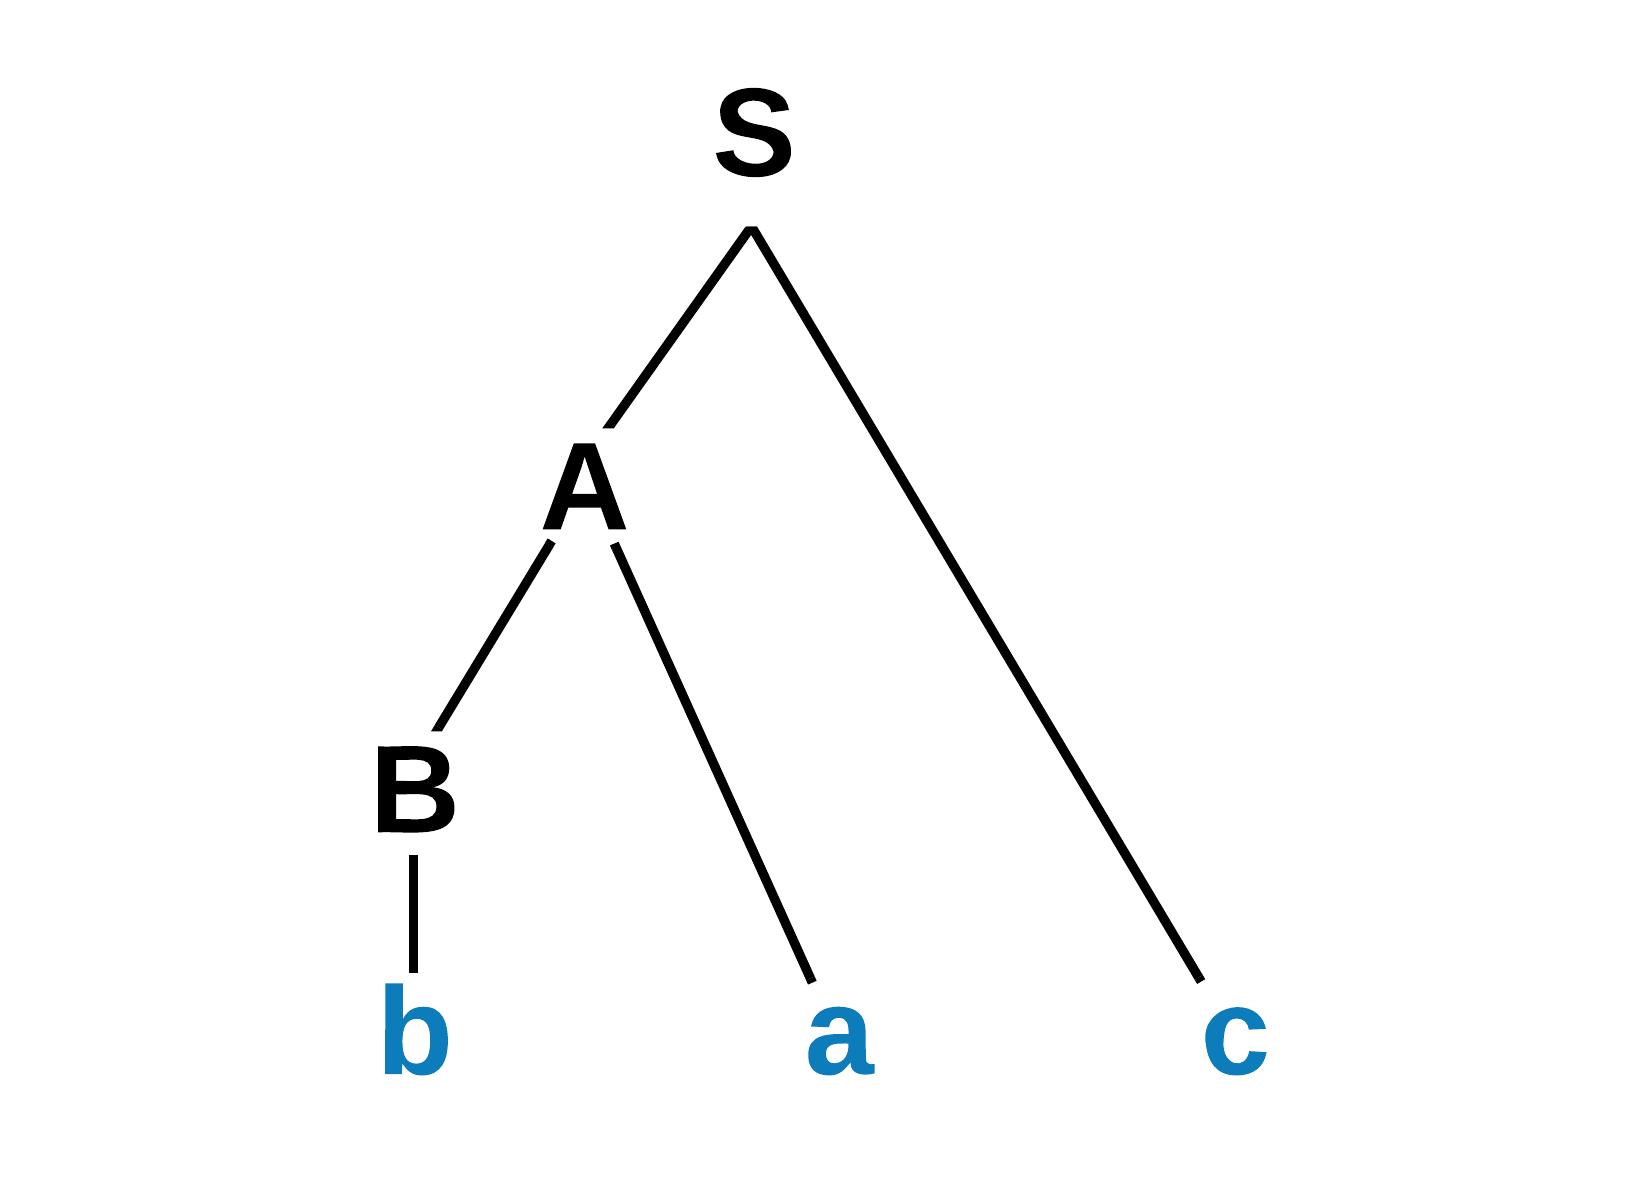
\includegraphics[width=0.5\textwidth]{obrazky-figures/derivationTree.png}
	\caption{Derivačný strom pre bezkontextovú gramatiku $G = (\{S, A, B\}, \{a, b, c\}, \{S\to Ax, A\to Ba, B\to b\}, S)$.}
	\label{derivationTree}
\end{figure}


\subsection{Chomského normálová forma}
\label{CNF}
Pri syntaktickej analýze popísanej v kapitole \ref{syntax} je veľmi dôležité vedieť formu, v akej sú jednotlivé pravidlá danej gramatiky. Pokiaľ je táto forma pravidiel vhodne obmedzená, umožní nám to použitie efektívnejších a sofistikovanejších algoritmov. Jednou z týchto foriem je práve Chomského normálová forma - \textit{CNF}.

\begin{definition}
\label{BKG}
Bezkontextová gramatika $ G = (N, T, P, S) $ je v \textit{Chomského normálovej forme} ak pre každé pravidlo $A \to x \in P $  platí $ x \in NN $ alebo $ x \in T $.


\end{definition}
\hfill\\
Prakticky to znamená, že na pravej strane pravidla sa môžu vyskytovať dva neterminály, alebo jeden terminál.
CNF sa obvykle spája s bezkontextovými gramatikami. Tento princíp však môžeme aplikovať aj pre pravidlá L-systémov.

Každú bezkontextovú gramatiku je možné transformovať do ekvivalentnej bezkontextovej gramatiky v Chomského normálovej forme \cite{medunaBase}. Preto pri práci s týmito gramatikami môžeme automaticky predpokladať, že sú práve v Chomského normálovej forme.

\subsection{Chomského hierarchia}
Rozlišujeme viacero druhov gramatík. Jednu z nich, bezkontextovú gramatiku (viď \ref{BKG}), sme si už popísali, ďalšie si len spomenieme. Tieto gramatiky je možné zoradiť podľa ich vyjadrovacej sily. Čím je gramatika silnejšia, tým viac unikátnych jazykov je pomocou nej možné popísať. Chomského hierarchia rozdeľuje gramatiky podľa ich vyjadrovacej sily do~štyroch rôznych úrovní nazývaných \textit{typ} spolu s číselným označením 0 až 3. Čím je číslo typu nižšie, tým silnejšia je daná gramatika.

\begin{definition}
\label{chomskyGrammars}
Gramatika $G = (N, T, P, S)$ sa označuje ako:

\begin{itemize}
    \itemsep0.2em 
    \item[] \textbf{kontextovo závislá} (anglicky \textit{context-sensitive}), ak pre každé prepisovacie pravidlo $u \to v \in P$ platí, že $u = u_1Au_2, v = u_1xu_2$ pre $u_1, u_2 \in (N \cup T)^*, A \in N, x \in (N \cup T)^+$ a taktiež sa označuje ako \textbf{CS}
    \item[] \textbf{bezkontextová}, ak pre každé prepisovacie pravidlo $u \to v \in P$ platí, že $u \in N$ a taktiež sa označuje ako \textbf{CF}
    \item[] \textbf{lineárna}, ak pre každé prepisovacie pravidlo $u \to v \in P$ platí, že $u \in N$ a $v \in T^* \cup (T^*NT^*)$ a taktiež sa označuje ako \textbf{LIN}
    \item[] \textbf{regulárna}, ak pre každé prepisovacie pravidlo $u \to v \in P$ platí, že $u \in N$ a $v \in T \cup TN \cup \{\epsilon\}$ a taktiež sa označuje ako \textbf{REG}
\end{itemize}

\end{definition}
\hfill\\

Frázové, kontextovo závislé, bezkontextové a regulárne gramatiky sa v Chomského hierarchii označujú ako gramatiky typu 0, typu 1, typu 2, typu 3 v tomto poradí \cite{handbook}.

\begin{definition}[Chomského hierarchia]
Platí nasledovná striktná inklúzia: \[L(REG) \subset L(LIN) \subset L(CF) \subset L(CS) \subset L(RE)\]

\end{definition}

$L()$ predstavuje rodinu jazykov generovanú jednou z gramatík, definovaných v definícii \ref{chomskyGrammars} a $L(RE)$ predstavuje rodinu \textit{rekurzívne vyčísliteľných} jazykov ktoré sú generované frázovými gramatikami.

Táto hierarchia je graficky reprezentovaná na obrázku \ref{chomskyGrammars}.

\begin{figure}[hbt]
	\centering
	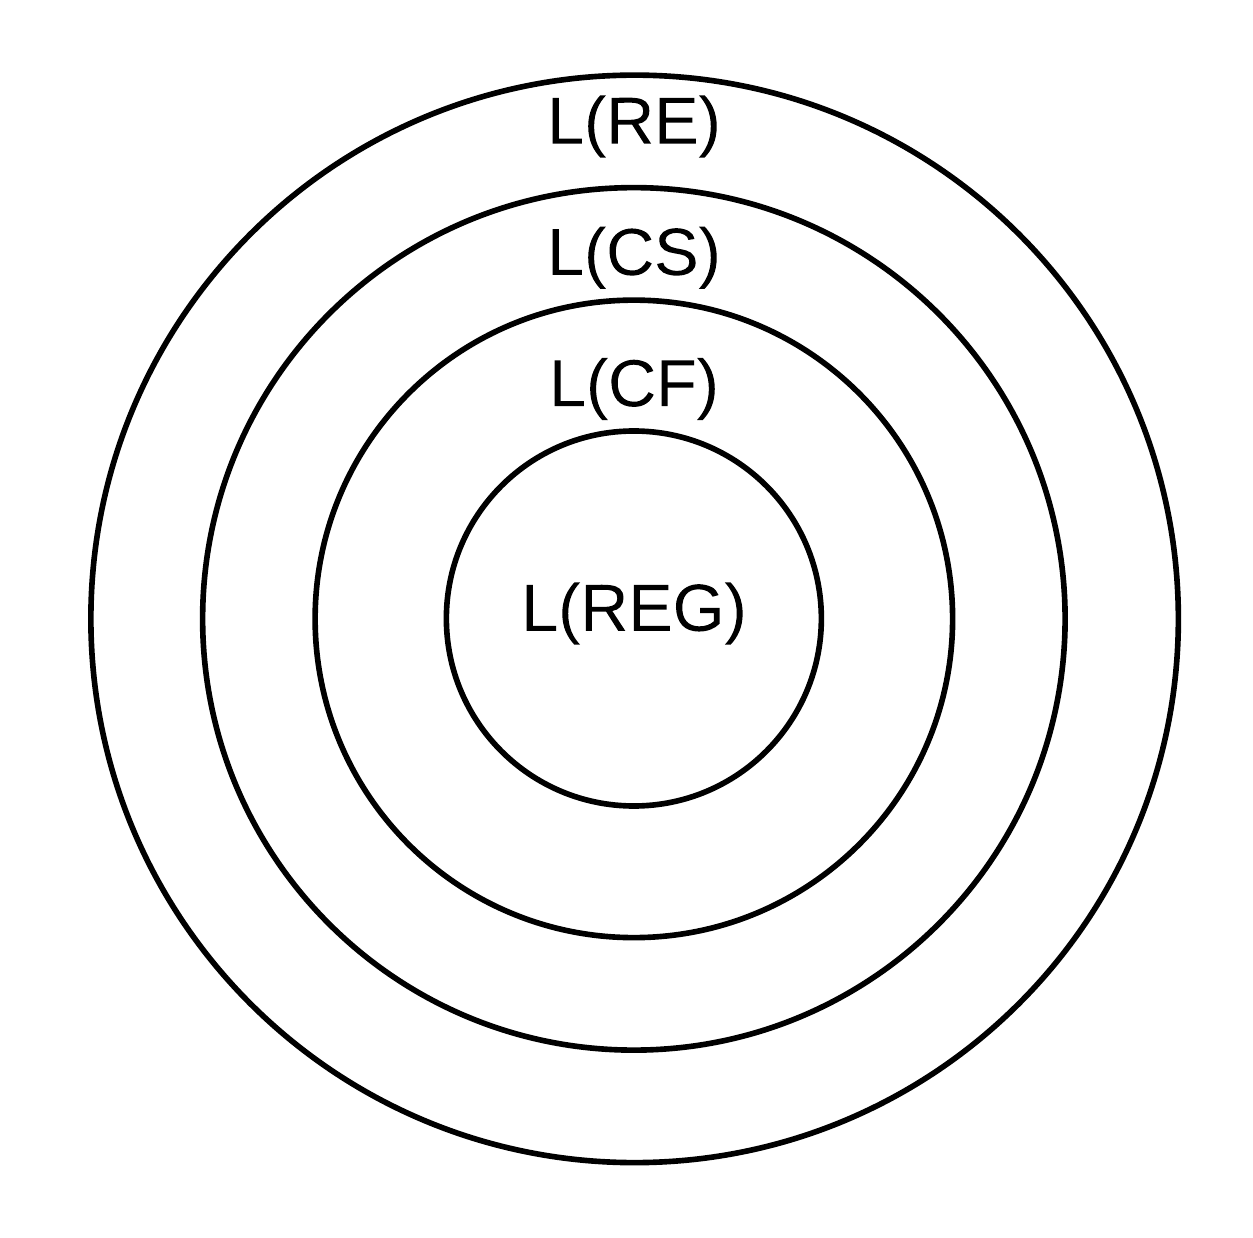
\includegraphics[width=0.5\textwidth]{obrazky-figures/chomskyHierarchy.png}
	\caption{Chomského hierarchia jazykov, kde L(RE), L(CS), L(CF), L(REG) značia rodinu rekurzívne vyčísliteľných, kontextovo závislých, bezkontextových a regulárnych jazykov v~tomto poradí.}
	\label{chomskyHierarchy}
\end{figure}

%=============================================================================================
\chapter{L-systémy}
\label{lsystem}

Lindenmayerove systémy, alebo skrátene L-systémy sú pomenované po biológovi Aristidovi Lindenmayerovi. Ten s ich konceptom prišiel v roku 1968. Boli vytvorené za účelom matematického popisu rastu rastlín a rôznych bunkových organizmov\cite{algBeauty}. Základ L-systémov vznikol samostatne, mimo teoretickú informatiku a až neskôr sa stal súčasťou teoretickej informatiky. Preto sa môžu vyskytovať rôzne inkonzistencie v názvosloví.

V praxi sú L-systémy dobre využiteľné. Umožňujú procedurálne generovať fraktály, rastliny, stromy a pod. Ďalšou výhodou je, že je možné generovať náhodné variácie spomínaných objektov. Preto je ich hlavné využitie v počítačovej grafike. Najčastejším použitím je teda generovanie reťazcov z L-systémov. V tejto práci sa venujeme opačnému problému. A to zisťovaniu, či boli reťazce vygenerované daným L-systémom.

Hlavnou a najpodstatnejšou vlastnosťou L-systémov, ktorou sa odlišujú od ostatných formálnych modelov, je ich \textbf{úplný paralelizmus}. To znamená, že v rámci každého derivačného kroku sa prepisujú všetky symboly slova.

V tejto práci sa zaujímame hlavne o ET0L systémy. Tento názov je zložený z viacerých vlastností L-systémov, ktoré si popíšeme v tejto kapitole.

\section{0L systémy}

Najjednoduchšou formou L-systémov sú práve 0L systémy. Jedná sa o bezkontextové L-systémy, čo značí \textbf{0} v názve (číta sa ako písmeno \uv{o}). Vo svojej podstate sú špeciálnou variantou obyčajných prepisovacích systémov \cite{salomaa} (viď \ref{rewrite}), ktoré ale ako už bolo spomenuté, v rámci svojho derivačného kroku aplikujú všetky možné pravidlá zároveň. Sú teda prepísané všetky znaky v pôvodnom slove.

Tak isto ako prepisovacie systémy, obsahujú len jednu abecedu, ktorá obsahuje len neterminály. Nerozlišujú sa teda terminály a neterminály, ako napríklad v gramatikách (viď \ref{grammar}). To znamená, že po každom derivačnom kroku získavame platný reťazec, ktorý patrí do generovaného jazyka.


\begin{definition}
\label{0L}

0L systém je trojica
\[ G = (\Sigma, P, w_o) \]
kde

\begin{itemize}
    \itemsep0.2em 
    \item[] $ \Sigma $ je abeceda;
    \item[] $ P $ je konečná množina \textit{produkcií} (pravidiel) v tvare $ (a, \alpha) \in P $ označované ako $ a \to \alpha $  \\ kde $ a \in \Sigma $ a $ \alpha \in \Sigma^* $;
    \item[] $ w_o $ je počiatočné slovo nad $ \Sigma$, $w_o \in \Sigma^+ $;
\end{itemize}
\end{definition}
\hfill\\


Produkcie (ďalej pravidlá) sa niekedy v literatúre označujú aj ako \textit{substitúcie}.
Počiatočné slovo $ w_o $ sa často označuje ako \textit{axiom}.


\begin{definition}
Pre 0L systém $G = (\Sigma, P, w_o)$ je \textbf{derivačný krok} $\Rightarrow$ definovaný nasledovne:
\[x_1...x_n \Rightarrow y_1...y_n, \quad\quad n\geq1 \text{ pre každé } x_i \in \Sigma \]

platí, že $x_i \to y_i \in P$ pre každé $i = 1,...,n$. Jazyk generovaný 0L systémom G je definovaný ako $L(G) = \{u | w \Rightarrow^*u\}$.

\end{definition}
\hfill\\

\subsection*{Vlastnosti uzavretí}
Keďže 0L systémy neobsahujú žiadnu formu filtrovania výsledných reťazcov, znamená to, že 0L systémy majú slabé vlastnosti uzavretí. Ináč povedané, nie sú uzavreté nad väčšinou jazykových operácií (viď \ref{closureProperties}).

0L systémy nie sú uzavreté nad týmito operáciami: \textit{zjednotenie, Kleene +, morfizmus, inverzný morfizmus, prienik s regulárnym jazykom, zreťazenie, doplnok} \cite{TIDPresentation}. Niektoré tieto operácie sú definované v časti \ref{closureProperties} a ostatné sú bežné množinové operácie. Porovnanie vlastností uzavretí s inými 0L rodinami je možné vidieť v tabuľke \ref{closurePropertiesTable}.

Rodina jazykov generovaná E0L systémami sa na základe svojich vlastností uzavretí klasifikuje ako \textit{anti-AFL}. Toto označenie je definované v definícii \ref{AFLDefinition}.

\subsection*{Porovnanie s Chomského hierarchiou}
Vďaka úplnému paralelizmu a slabým vlastnostiam uzavretí majú 0L systémy špecifický vzťah ku formálnym gramatikám, pokiaľ porovnávame ich vyjadrovaciu silu.

Rodina jazykov generovaná 0L systémom má prienik s niektorými rodinami v~Chomského hierarchii, konkrétne s rodinami bezkontextových a regulárnych jazykov. Je však podmnožinou kontextovo závislých jazykov. To znamená, že bezkontextové a regulárne rodiny jazykov obsahujú také jazyky, ktoré neobsahuje rodina jazykov 0L. A naopak, 0L rodina jazykov obsahuje jazyky, ktoré neobsahujú rodiny bezkontextových a regulárnych jazykov. Túto hierarchiu aj s príkladmi jazykov je možné vidieť na obrázku \ref{0LHierarchy}.

\begin{figure}[hbt]
	\centering
	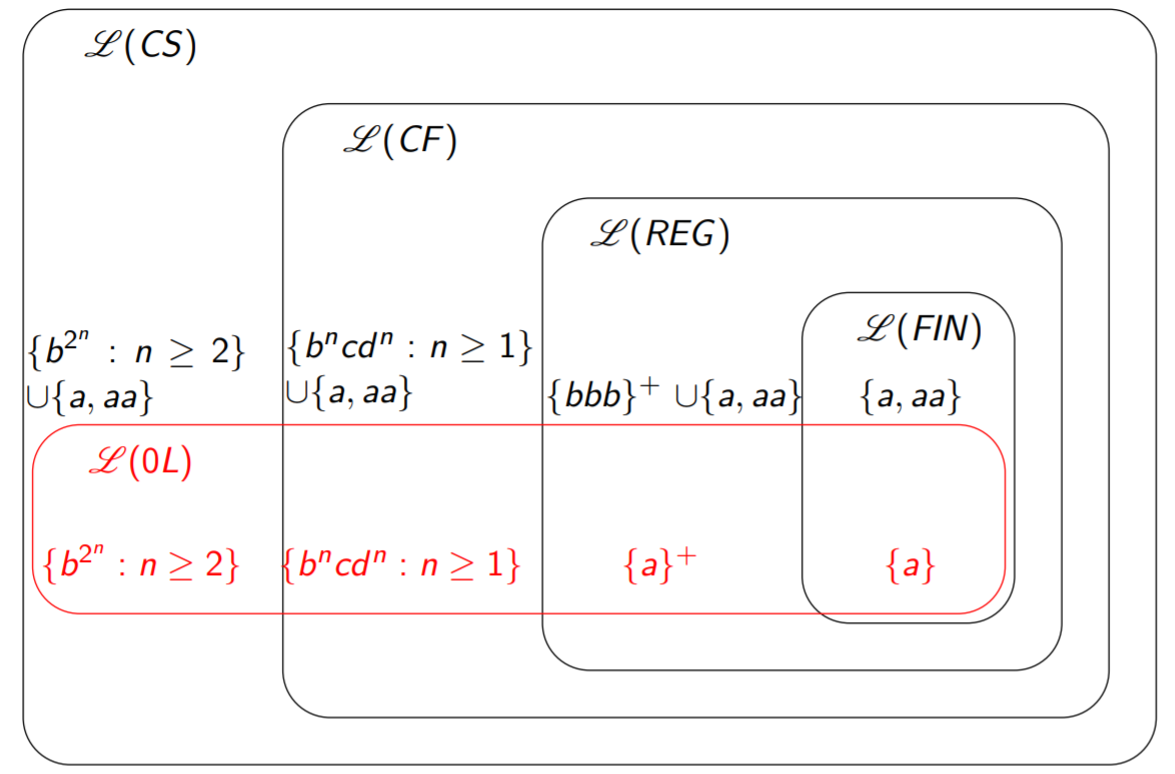
\includegraphics[width=0.8\textwidth]{obrazky-figures/0Lhierarchy.png}
	\caption{0L systémy v kontexte Chomského hierarchia jazykov, kde L(CS), L(CF), L(REG), L(FIN) značia rodinu kontextovo závislých, bezkontextových, regulárnych a konečných jazykov v tomto poradí. Ďalej sú uvedené príklady jazykov ktoré nepatria do rodiny jazykov 0L. Obrázok je prebraný z prezentácie \cite{TIDPresentation}.}
	\label{0LHierarchy}
\end{figure}

\section{Rodiny}
\label{0LFamilies}
0L systémy vo svojej základnej podobe neobsahujú žiadne filtrovacie mechanizmy, musíme teda prijať všetky reťazce vygenerované týmito systémami \cite{handbook}. Táto vlastnosť je však veľmi obmedzujúca, je teda potrebné tento problém vyriešiť. Riešením je zavedenie rôznych filtrovacích mechanizmov. Príkladom takéhoto filtrovania je používanie neterminálov. Tento spôsob používajú napríklad gramatiky (viď \ref{grammar}), ktoré neprijmú reťazec, pokiaľ sa v ňom vyskytuje aspoň jeden neterminál. Ich jazyk teda obsahuje iba také slová, kde je každý ich symbol neterminál.

Takéto filtrovanie do 0L systémov zavádzame pomocou \textit{rodín}. Tieto rodiny rôzne modifikujú 0L systémy, buď rozšíreniami, alebo naopak obmedzeniami. To znamená, že filtrácia je len jedným z dôvodov, prečo sa tieto rodiny používajú.

Rodiny 0L systémov sa označujú pomocou písmena pred označením 0L. Tie sa navyše môžu rôzne kombinovať. Takže rodina ET0L, ktorou sa zaoberáme, znamená kombináciu rodín E a T 0L systémov. To však neznamená, že tieto rodiny sa používajú len pre 0L systémy. Používajú sa aj pre kontextovo závislé L-systémy, kde sa taktiež uvádzajú na~začiatku označenia.

\subsection*{D - deterministic}
Základnou rodinou, ktorá sa v literatúre uvádza sú D0L systémy. Pre rodinu D platí, že množina pravidiel $ P $ obsahuje pre každé $ a \in \Sigma $ práve jedno pravidlo.

Algoritmus pre syntaktickú analýzu (viď \ref{CYK}), ktorý modifikujeme v rámci tejto práce, však zvláda aj nedeterministické gramatiky. Preto sa pri jeho modifikácii pre L-systémy nemusíme obmedzovať determinizmom a tak túto rodinu nepoužívame.

\subsection*{P - propagating}
Táto rodina 0L systémov odstraňuje prázdne prepisovacie pravidlá. Teda pravidlá v tvare $\alpha \to \epsilon$.

V tejto práci sa touto rodinou priamo nezaoberáme, používa sa však v inom existujúcom riešení.

\subsection*{E - extended}
\label{extended}
Pri definícii 0L systému bolo spomenuté, že neobsahujú neterminály. Táto rodina rozširuje 0L systémy práve o neterminály a tým nám umožňuje filtrovať výsledné reťazce. E0L systémy tak majú vyššiu vyjadrovaciu silu než klasické 0L systémy.

Filtrovanie na základe neterminálov funguje tak, že generovaný jazyk nemôže obsahovať reťazce, ktoré obsahujú aspoň jeden neterminál.

Zavedením rodiny E0L získavame systémy veľmi podobné bezkontextovým gramatikám. Rozdiel je v už spomínanej paralelnej aplikácii pravidiel.


\subsection*{T - tables}
\label{tables}
Najvýraznejšou modifikáciou 0L systémov oproti formálnym gramatikám (viď \ref{grammar}) je práve rodina T. Tá zavádza množinu tabuliek pravidiel. Pri každom derivačnom kroku je možné zvoliť tabuľku, z ktorej sa budú pravidlá aplikovať. Tabuľka nie je nič iné, než konečná množina produkcií $P$.

Motivácia zavedenia viacerých tabuliek pravidiel pochádza z premenlivých podmienok pre vývoj rastlín a organizmov. Tými môžu byť rôzne časti dňa, roka alebo odlišné fázy rastu \cite{handbook}.

Táto vlastnosť má zmysel len pri paralelnom prepisovaní. Nakoľko pri sekvenčnom prepisovaní aplikujeme pravidlá jednotlivo, nemá zmysel voliť medzi rôznymi tabuľkami \cite{handbook}.


\hfill\\
Existuje mnoho ďalších rodín 0L systémov. Niektoré z nich zavádzajú spôsoby filtrovania reťazcov, pri ktorých je možné skúmať a porovnávať ich vyjadrovaciu silu. Nimi sa v tejto práci zaoberať nebudeme. 


\section{E0L systémy}
V predchádzajúcej časti \ref{0LFamilies} bola definovaná rodina E 0L systémov ako rozšírenie o~neterminály. E0L systém je teda taký 0L systém, kde je abeceda $\Sigma$ rozdelená na dve disjunktné časti, pričom jedna časť obsahuje terminály a druhá časť obsahuje neterminály. Ako už bolo spomenuté, jazyk generovaný E0L systémom obsahuje len také slová, ktoré neobsahujú neterminály.

Pri popisovaní rodín 0L systémov bolo spomenuté, že tieto rodiny je možné kombinovať a dopracovať sa tak až k ET0L systémom. Preto je definovaný aj E0L systém ako medzikrok, aby sa bolo možné sa prepracovať až k ET0L systémom, ktoré sú hlavným predmetom tejto práce.


\begin{definition}
\label{E0LDefinition}

E0L systém je štvorica

\[ E = (\Sigma, T, P, w_o) \]

kde 

\begin{itemize}
    \itemsep0.2em 
    \item[] $\Sigma$ je celková abeceda
    \item[] $T$ je abeceda terminálov, $ T \subseteq \Sigma $
    \item[] $ P $ je konečná množina \textit{produkcií} (pravidiel) v tvare $ (a, \alpha) \in P $ označované ako $ a \to \alpha $  \\ kde $ a \in \Sigma $ a $ \alpha \in \Sigma^* $;
    \item[] $ w_o $ je počiatočné slovo nad $ \Sigma$, $w_o \in \Sigma^+ $;
\end{itemize}
\end{definition}
\hfill\\

Keďže E0L systémy zavádzajú pomocou abecedy terminálov spôsob filtrovania výsledných slov, zvyšuje sa tým ich vyjadrovacia sila oproti 0L systémom. Rodina jazykov generovaná E0L systémami má taktiež lepšie vlastnosti uzavretí ako 0L systémy. To~znamená, že je uzavretá nad viacerými jazykovými operáciami.

\subsection*{Vlastnosti uzavretí}
Ako bolo spomenuté, modifikáciou E nad 0L systémami sa zlepšujú vlastnosti uzavretí rodiny jazykov E0L systémov. Stáva sa takmer \textit{plne AFL}, je však neuzavretá nad \textit{inverzným morfizmom}.

\subsection*{Porovnanie s bezkontextovou gramatikou}
Pri 0L systémoch bolo spomenuté, že rodina 0L jazykov má prienik s rodinou bezkontextových jazykov. Teda obe obsahujú jazyky, ktoré neobsahuje druhá rodina, neplatí medzi nimi inklúzia. E0L systémy však majú vyššiu vyjadrovaciu silu než 0L systémy a~platí inklúzia $L(CF) \subset L(E0L) \subset L(CS)$, kde $L(CF)$ značí bezkontextovú rodinu jazykov generovanú bezkontextovými gramatikami.

\begin{definition}
\label{BKGtoE0L}
Pre každú bezkontextovú gramatiku $G = (N, T, P, S)$ platí, že ak pre každý symbol $\alpha \in N \cup T$ pridáme prepisovacie pravidlo $\alpha \to \alpha$ a výsledok budeme vnímať ako E0L systém $G_1$, platí jazyková ekvivalencia $L(G) = L(G_1)$.
\end{definition}
\hfill\\
Táto definícia poukazuje na vlastnosť, že každú bezkontextovú gramatiku je možné vyjadriť ekvivalentným E0L systémom\cite{salomaa}.

\section{ET0L systémy}
Najviac študovanou rodinou L-systémov sú práve ET0L systémy vďaka svojím vhodným matematickým vlastnostiam a silným vlastnostiam uzavretí nad operáciami (anglicky \textit{closure properties}).
Ako bolo spomenuté, jednotlivé rodiny je možné kombinovať, takže ET0L systém je rozšírením 0L systému o abecedu neterminálov a množiny tabuliek pravidiel. Je to kombinácia rodín E (extended) a T (tables).

\begin{definition}
\label{ET0LDefinition}
ET0L systém je (n + 3)-tica

\[ E = (\Sigma, T, P_1, P_2, ..., P_n, w_o) \]

kde 

\begin{itemize}
    \itemsep0.2em 
    \item[] $n \geq 1$
    \item[] pre všetky $ i = 1, ..., n$, $E_i = (V, T, P_i, w)$ je E0L systém
\end{itemize}
\end{definition}
\hfill\\

Predpokladáme, že každá tabuľka obsahuje pre každé $ a \in \Sigma $ aspoň jedno pravidlo.

\subsection*{Počet tabuliek}
ET0L systémy nijako neobmedzujú počet tabuliek, ktoré obsahujú. Môžu teda teoreticky obsahovať nekonečno týchto tabuliek. Vyplýva teda otázka, ako sa menia vlastnosti ET0L systémov v závislosti na počte týchto tabuliek.

Na počte tabuliek v ET0L systémoch nezáleží. Platí totiž, že pre každý ET0L systém existuje ekvivalentný ET0L systém s \textbf{dvoma tabuľkami}\cite{handbook}.

\subsection*{Derivačný krok}
Pri každej aplikácii pravidiel, teda pri \textbf{derivačnom kroku}, je nutné vybrať si jednu z~tabuliek pravidiel, z ktorej sa budú tieto pravidlá používať. Neexistuje žiadne pravidlo, ktoré by hovorilo, ktorá tabuľka má byť, alebo naopak, nemôže byť použitá. Môže byť teda vybratá ľubovoľná tabuľka $P_i$. V rámci daného derivačného kroku sa však môžu aplikovať pravidlá iba z jednej tabuľky.

\begin{definition}
Pre ET0L systém $G = (\Sigma, T, P_1, ..., P_n, w_o)$  je \textbf{derivačný krok} $\Rightarrow$ definovaný nasledovne:
\[x_1...x_n \Rightarrow y_1...y_n, \quad\quad n\geq1 \text{ pre každé } x_i \in \Sigma \]

platí, že $x_i \to y_i \in G_k = (\Sigma, T, P_k, w_o)$ pre každé $i = 1,...,n$. Pričom $G_k$ je E0L systém podľa definície \ref{ET0LDefinition}.
\end{definition}

\subsection*{Vlastnosti uzavretí}
Zavedením rodiny T k už existujúcim E0L systémom sa zlepšujú aj vlastnosti uzavretí týchto L-systémov. Konkrétne, ET0L systémy sa označujú ako \textit{plne AFL}, čo znamená, že oproti E0L systémom sú navyše uzavreté nad operáciou inverzného morfizmu. Pokiaľ uvažujeme rodinu T0L, teda bez rodiny E, tak ide o \textit{anti AFL} rodinu, rovnako ako je to pri 0L systémoch\cite{handbook}.

\subsection*{Porovnanie s Chomského hierarchiou}
Rozšírenie E0L systémov o rodinu T zvyšuje vyjadrovaciu silu výsledných ET0L systémov podobne, ako sa zlepšili ich vlastnosti uzavretí. Stávajú sa tak nadmnožinou E0L systémov, ale stále majú nižšiu vyjadrovaciu silu, než rodina kontextovo závislých jazykov a sú ich podmnožinou. Platí teda vzťah:
\[L(CF) \subset L(E0L) \subset L(ET0L) \subset L(CS)\]
Porovnanie vlastností uzavretí gramatík z Chomského hierarchie a L-systémov definovaných v tejto kapitole je možné vidieť v tabuľke \ref{closurePropertiesTable}.

\begin{table}[]
    \centering
    \begin{tabular}{|c||c|c|c|c||c|c|c|}
    \hline
        & RE & CS & CF & REG & 0L & E0L & ET0L\\
    \hline
        Zjednotenie & $\checkmark$ & $\checkmark$ & $\checkmark$ & $\checkmark$ 
        & $\times$ & $\checkmark$ & $\checkmark$ \\
    \hline
        Prienik & $\checkmark$ & $\checkmark$ & $\times$ & $\checkmark$
        &  &  &  \\
    \hline
        Doplnok & $\times$ & $\checkmark$ & $\times$ & $\checkmark$
        & $\checkmark$ & $\checkmark$ & $\checkmark$ \\
    \hline
        Zreťazenie & $\checkmark$ & $\checkmark$ & $\checkmark$ & $\checkmark$
        & $\times$ & $\checkmark$ & $\checkmark$ \\
    \hline
        Kleene star (*) & $\checkmark$ & $\checkmark$ & $\checkmark$ & $\checkmark$
        & $\times$ & $\checkmark$ & $\checkmark$ \\
    \hline
        Substitúcia & $\checkmark$ & $\times$ & $\checkmark$ & $\checkmark$
        &  &  &  \\
    \hline
        Morfizmus & $\checkmark$ & $\times$ & $\checkmark$ & $\checkmark$
        & $\times$ & $\checkmark$ & $\checkmark$ \\
    \hline
        Inverzný morfizmus & $\checkmark$ & $\checkmark$ & $\checkmark$ & $\checkmark$
        & $\times$ & $\times$ & $\checkmark$ \\
    \hline
    \end{tabular}
    \caption{Vlastnosti uzavretí rodín jazykov z Chomského hierarchie a rodín jazykov L systémov. Prevzaté z knihy \cite{handbook} a prezentácie \cite{TIDPresentation}.}
    \label{closurePropertiesTable}
\end{table}

\section{Chomského normálová forma E0L a ET0L systémov}
\label{chomskyDegradation}
Pri bezkontextových gramatikách bola definovaná aj ich Chomského normálová forma \ref{CNF}. V skratke sa jedná o tvar pravidiel, do ktorého je možné transformovať ľubovoľnú bezkontextovú gramatiku, pričom výsledná gramatika jej bude ekvivalentná. Táto forma sa využíva pri algoritme Cocke-Younger-Kasami (viď \ref{CYK}). Preto je v rámci tejto práce Chomského normálová forma žiadaná aj pre E0L a ET0L systémy. Umožňuje totiž pomocou istých modifikácií využiť spomínaný algoritmus CYK aj pre tieto systémy.

0L systémy všeobecne obsahujú prepisovacie pravidlá pre terminály (0L systémy nerozoznávajú terminály a neterminály, všetky symboly sa môžu považovať za terminály). Pri bezkontextových gramatikách takéto pravidlá neexistujú, prepisujú sa teda len neterminály. Chomského normálová forma teda s takýmito pravidlami nepočíta. Preto v~prípade E0L a ET0L systémov musíme uvažovať implicitné pravidlo $\alpha \to \alpha$, ináč povedané, terminály sa neprepisujú. Ignorujú sa. Ďalej sa obmedzí axiom na počiatočný symbol z~abecedy neterminálov.

\subsection*{Degradácia vyjadrovacej sily použitím Chomského normálovej formy}


Zavedenie tejto normálovej formy však spôsobuje vážny problém pre E0L a následne aj pre ET0L systémy. Ten vyplýva z definície \ref{BKGtoE0L}. Pokiaľ zapíšeme pravidlá v Chomského normálovej forme a pre terminály uvažujeme spomínané implicitné pravidlo $\alpha \to \alpha$, získavame tak E0L systém, ktorý je ekvivalentný bezkontextovej gramatike s rovnakými pravidlami. Znamená to, že pri použití tejto normálovej formy degradujeme vyjadrovaciu silu E0L systémov na tú bezkontextových gramatík. To ovplyvní aj ET0L systémy.

\section{Normálová forma E0L a ET0L systémov}
\label{E0LNormalForm}
Existuje normálová forma, pomocou ktorej je možné pre každý E0L systém vyjadriť ekvivalentný E0L systém. Táto normálová forma obsahuje pravidlá v nasledovnom tvare:

\[
    A \to a, \quad\quad A \to B, \quad\quad A \to BC, \quad\quad a \to A, \quad\quad A \to \epsilon; \quad \quad
\]

kde $A$, $B$, $C$ sú ľubovoľné neterminály a $a$ je ľubovoľný terminál. Táto normálová forma je prevzatá z knihy \cite{mathTheoryL}.

V definícii ET0L systémov \ref{ET0LDefinition} je ET0L systém definovaný pomocou E0L systémov. Pre každú tabuľku, ktorú obsahuje, existuje E0L systém. Preto pokiaľ transformujeme každú tabuľku do tejto normálovej formy, získame ekvivalentný ET0L systém.

Oproti Chomského normálovej forme sa táto normálová forma líši prepisovaním jedného terminálu na neterminál alebo naopak. Taktiež sú povolené takzvané prázdne prepisovacie pravidlá, teda prepisovaný neterminál sa vymaže. To je značené symbolom $\epsilon$.



\section{Kontextová závislosť}
V rámci tejto kapitoly sa rozoberali len bezkontextové L-systémy, v ktorých sa táto bezkontextovosť označuje pomocou \uv{0} v názve. Za zmienku však stoja aj kontextovo závislé L-systémy, ktoré sa označujú ako \textbf{interaktívne L-systémy} a skratkou \textbf{IL systémy} kde \uv{\textit{I}} znamená interaktívnosť. 

Kontextovosť sa označuje ako $(m, n)L$ systém, kde $m, n \geq 0$ a má pravidlá v tvare\cite{handbook}
\[ (\alpha, a, \beta) \to w \quad\text{kde}\quad |\alpha|=m, |\beta|=n \]

Z tohto tvaru pravidiel je zjavné, že prvé číslo $m$ v zátvorke značí počet symbolov, ktoré sú vnímané ako súčasť kontextu na ľavej strane prepisovaného symbolu a druhé číslo $n$ značí zasa pravú stranu.

Kontextová závislosť pri bezkontextových L-systémoch by sa teda v tejto notácii značila ako (0, 0). Toto značenie sa však skracuje na \textbf{0}.

%=============================================================================================
\chapter{Syntaktická analýza} 
\label{syntax}

S niektorými formami syntaktickej analýzy sa v informatike, hlavne pri programovaní, stretávame pravidelne. Pri prirodzených jazykoch môžeme za istú formu syntaktickej analýzy považovať kontrolu gramatiky a vetnej skladby. Túto kontrolu vykonáva človek, ktorý dokáže zmyslu vety porozumieť aj napriek istému počtu chýb. Na rozdiel od ľudí však počítač potrebuje presnú formu jazyka, ktorému má rozumieť a vyžaduje jeho striktné dodržiavanie.

V informatike sa syntaktická analýza používa v prekladačoch programovacích jazykov a tvorí ich hlavnú časť. Programovacie jazyky majú presne definovanú syntax, preto je možné ju použitím špecifických algoritmov kontrolovať. Nie všetky aspekty programovacích jazykov je možné vyjadriť formálne pomocou nejakej formy zápisu, preto sa v praxi bežne kombinuje syntaktická analýza so sémantickou analýzou. Príkladom môže byť kontrola existencie premenných.

V tejto práci sa venujeme samostatnej syntaktickej analýze. Jej cieľom je zistiť, či prijímaný reťazec patrí do jazyka, ktorý je generovaný daným formálnym modelom (viď \ref{formalModel}), konkrétne L-systémom. Ináč povedané, má za úlohu zistiť, či je možné pomocou konkrétnej gramatiky, prepisovacieho systému, alebo iného modelu, vygenerovať požadovaný reťazec.

\section{Druhy syntaktickej analýzy}
\label{analysysTypes}
Existuje mnoho rôznych algoritmov pre syntaktickú analýzu, ktoré môžeme rozdeliť do~dvoch hlavných skupín. Toto rozdelenie je na základe toho, akým spôsobom sa snažíme k~výsledku dopracovať. Algoritmus môže začať počiatočným symbolom a snažiť sa aplikáciou pravidiel získať výsledne slovo. Druhou možnosťou je presne opačný postup, kedy algoritmus začína celým slovom a snaží sa spätne zistiť, či mohlo byť vygenerované pomocou počiatočného symbolu.



\subsection*{Analýza zhora-dole}
Ako vrch a spodok implikovaný z názvu chápeme vrch a spodok derivačného stromu. Myšlienkou takejto analýzy (anglicky \textit{top-down}) je prepracovať sa aplikáciou prepisovacích pravidiel z počiatočného symbolu až ku kontrolovanému reťazcu. Tieto analýzy bývajú oproti analýzam zdola-hore jednoduchšie. Postupne generujú všetky možnosti a snažia sa nájsť zhodu. Často pri tom využívajú rekurziu.

Príkladom je algoritmus \textit{recursive descent}, ktorý sa využíva pri syntaktickej analýze programovacích jazykov.

Vizuálnu reprezentáciu tohto spôsobu je možné vidieť na obrázku \ref{topDownPicture}.

\begin{figure}[hbt]
	\centering
	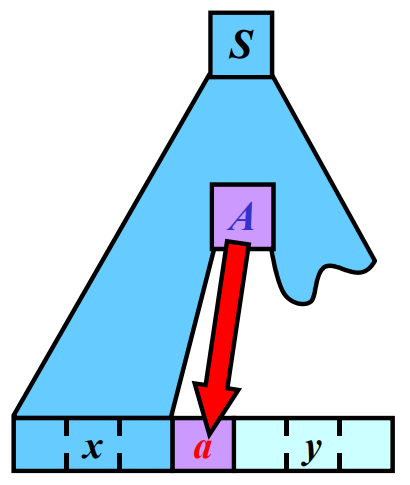
\includegraphics[width=0.3\textwidth]{obrazky-figures/topDown.png}
	\caption{Vizuálna reprezentácia princípu syntaktickej analýzy zhora-dole. Obrázok je prevzatý z prezentácie \cite{IFJPresentation}.}
	\label{topDownPicture}
\end{figure}

\subsection*{Analýza zdola-hore}
Tento spôsob syntaktickej analýzy sa v angličtine označuje ako \textit{bottom-up parsing}. Spodok z~názvu implikovaného derivačného stromu predstavuje reťazec, ktorý kontrolujeme. Znamená to, že sa snažíme spätne prepracovať z reťazca naspäť na vrch derivačného stromu. Ináč povedané ku počiatočnému symbolu. Tieto algoritmy bývajú efektívnejšie, nakoľko nemusia prechádzať všetky variácie derivačného stromu.

Príkladom takéhoto algoritmu je precedenčná analýza používaná na preklad výrazov.
\hfill\\

Oba spomenuté spôsoby syntaktickej analýzy sú bežne používané. Nie je možné povedať, ktorý z nich je lepší, nakoľko oba sú vhodné na iné druhy problémov. Preto sa napríklad v~rámci jedného prekladača bežne vyskytujú oba tieto spôsoby syntaktickej analýzy.

\section{Algoritmus Cocke-Younger-Kasami}
\label{CYK}
Jedná sa o algoritmus zo skupiny syntaktických analýz zdola-hore. To znamená, že postupnými redukciami výsledného slova pomocou prepisovacích pravidiel sa snaží prepracovať až k~počiatočnému znaku. Tento algoritmus bol zvolený ako základ pre~syntaktickú analýzu ET0L systémov. Neskôr je v rámci tejto kapitoly popísané, aké zmeny je potrebné vykonať, aby tento algoritmus dokázal spracovávať aj ET0L systémy.

Algoritmus Cocke-Younger-Kasami (ďalej len CYK) vykonáva syntaktickú analýzu bezkontextových gramatík. Podmienkou, aby mohol byť algoritmus CYK vykonaný je, aby bola vstupná gramatika v Chomského normálovej forme (viď \ref{CNF}). To v skratke znamená, že na pravej strane prepisovacích pravidiel môžu byť len dva neterminály alebo jeden terminál.

Vďaka tomu, že vstupná gramatika musí byť v Chomského normálovej forme, môže byť táto vlastnosť vhodne využitá algoritmom CYK. V tabuľke, s ktorou algoritmus CYK pracuje, sa vyhľadávajú práve dvojice vyplývajúce z Chomského normálovej formy.

Dôležitou vlastnosťou algoritmu CYK je, že zvláda nedeterministické gramatiky. Vstupná gramatika teda môže obsahovať viac pravidiel pre jeden neterminál.


\subsection*{Popis fungovania}

Pri vysvetlení algoritmu sú použité symboly bezkontextových gramatík z definície \ref{BKG} a~predpokladáme bezkontextovú gramatiku $G = (N, T, P, S)$, ktorá slúži ako vstupná gramatika.
Ako bolo spomenuté, algoritmus CYK pracuje na báze zdola-hore, teda analýza začína vstupným slovom $w$ a snaží sa dopracovať až k počiatočnému symbolu $S$.

Zavádza sa tabuľka $CYK[i, j]$, kde $1 \leq i \leq j \leq n$, pričom $n$ je dĺžka vstupného slova $w$. Táto tabuľka sa počas vykonávania algoritmu využíva na vyhľadávanie dvojíc pravých strán pravidiel. Pri nájdení takej dvojice nastáva redukcia pravidla na jeho ľavú stranu (podľa Chomského normálovej formy jeden neterminál) a daný neterminál sa zapíše do tabuľky.

Na úplnom začiatku je nutné do tabuľky $CYK$ vložiť vstupné slovo $w$. To funguje tak, že na diagonálu tabuľky $CYK$ sa umiestnia neterminály, pomocou ktorých je možné priamo derivovať (viď \ref{derivation}) neterminál na rovnakej pozícii vo vstupnom slove $w$. Využité je pravidlo z Chomského normálovej formy, kde je na pravej strane jeden terminál. Pre každé $A \in CYK[i, i]$ platí, že $A \to w_i \in P$ pričom $w_i$ je i-ty znak vo vstupnom slove $w$.

Potom sa v tabuľke CYK vyhľadávajú také dvojice neterminálov, kde platí $B \in CYK[i, j], C \in CYK[j+1, k]$ a $A \to BC \in P$, potom zapíšeme A do CYK[i, k]. Keďže sú bezkontextové gramatiky sekvenčné, každý zapísaný neterminál je používaný v nasledovnom hľadaní dvojíc. Toto hľadanie dvojíc sa vykonáva dovtedy, kým je možné nájsť novú, teda unikátnu dvojicu.

Algoritmus je úspešný, pokiaľ sa nachádza počiatočný symbol $S$ v CYK[1, n]. Vysvetlenie algoritmu je parafrázované z knihy \cite{medunaParser}. Popis algoritmu CYK pre bezkontextové gramatiky je ekvivalentne popísaný pomocou pseudokódu \ref{CYKBKG}. Príkladná vizualizácia fungovania tohto algoritmu je viditeľná na obrázku \ref{CYKTable}.

\hfill\\
Každú bezkontextovú gramatiku je možné previesť na ekvivalentnú bezkontextovú gramatiku v Chomského normálovej forme \cite{medunaBase}. To znamená, že tento algoritmus je možné aplikovať na ľubovoľnú bezkontextovú gramatiku, ktorú je však najprv nutné previesť do~Chomského normálovej formy.


\begin{figure}[hbt]
	\centering
	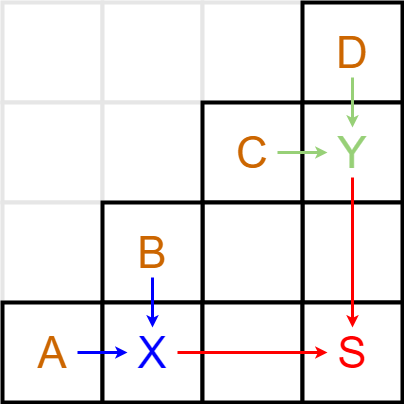
\includegraphics[width=0.3\textwidth]{obrazky-figures/CYKTable.png}
	\caption{Príklad úspešného vykonania algoritmu CYK s vizualizáciou tabuľky CYK pre gramatiku $G = (\{A, B, C, D, X, Y, S\}, \{a, b, c, d\}, \{S \to XY, X \to AB, Y \to CD, A \to a, B \to b, C \to c, D \to d, S\})$ pre~vstupné slovo $abcd$. Spodný ľavý roh predstavuje pozíciu [1, 1] a spodný pravý roh pozíciu [1,4] v tabuľke CYK.}
	\label{CYKTable}
\end{figure}

\begin{algorithm}
\caption{Algoritmus syntaktickej analýzy Cocke-Younger-Kasami pre bezkontextové gramatiky}
\label{CYKBKG}

\textbf{Input}
\setlist{nolistsep}
\begin{itemize}[noitemsep]
    \item grammar, \(G = ({}_G\Sigma, {}_GR)\) in Chomsky normal form
    \item \(w = a_1a_2...a_n\)  where  \(a_i \in {}_G\Delta, 1 \leq i \leq n \), for some \(n \geq 1\).
\end{itemize}
\textbf{Output} 
\begin{itemize}[noitemsep]
    \item \textbf{ACCEPT} if \(w \in L(G)\)
    \item \textbf{REJECT} if \(w\notin L(G)\)
\end{itemize}
\textbf{Method}
\begin{algorithmic}
\State $ CYK[i,j] = \varnothing$ for $1 \leq i \leq j \leq n $
\For{i = i \textbf{to} $n$}
    \If{$ A \rightarrow a_i \in R $}
        \State $add\ A\ to\ CYK[i,i]$
    \EndIf
\EndFor
\Repeat
\If{$ B \in CYK[i,j], C \in CYK[j+1,k], A \rightarrow BC \in R $ for some $A,B,C \in {}_GN$}
\State $add\ A\ to\ CYK[i,k]$
\EndIf
\Until{no changes}
\If{$ S \in CYK[1,n] $}
    \State \textbf{ACCEPT}
\Else
    \State \textbf{REJECT}
\EndIf

\end{algorithmic}
\end{algorithm}

\section{CYK pre rôzne 0L systémy}
Hlavný rozdiel 0L systémov oproti bezkontextovým gramatikám je paralelná aplikácia pravidiel na rozdiel od sekvenčnej aplikácie pravidiel bezkontextových gramatík. To~znamená, že všetky pravidlá musia byť aplikované zároveň. Algoritmus \textit{CYK} je možné vhodnou modifikáciou upraviť tak, aby túto skutočnosť reflektoval.

Dôležitým rozdielom je aj používaná normálová forma. Algoritmus CYK pracuje s~bezkontextovými gramatikami v Chomského normálovej forme. Táto forma pravidiel však nevyhovuje pre použitie s E0L a ET0L systémami, nakoľko obmedzuje ich vyjadrovaciu silu. Preto je používaná normálová forma definovaná v časti \ref{E0LNormalForm}. Rozdiely v tejto normálovej forme oproti Chomského normálovej forme je potrebné zohľadniť pri modifikácii algoritmu CYK. Unárne pravidlá tejto normálovej formy môžeme generalizovať na tvar $\alpha \to \alpha$, pričom $\alpha$ je ľubovoľný znak z celkovej abecedy $\Sigma$.


Ďalším rozdielom, ktorým sa zaoberáme, sú tabuľky (viď \ref{tables}) ET0L systémov. Pre tieto systémy platí, že pred každou aplikáciou pravidiel je zvolená tabuľka pravidiel a pri aplikácii pravidiel sa používajú len pravidlá, ktoré patria do danej tabuľky. Túto vlastnosť je tak isto možné vhodnou modifikáciou algoritmu \textit{CYK} aplikovať.

Podobne ako môžeme kombinovať rôzne rodiny 0L systémov, môžeme kombinovať aj syntaktickú analýzu pre zložené rodiny, napríklad ET0L, a aplikovať v nej modifikácie pre~každú rodinu z ktorej sa skladá. V našom prípade to znamená modifikovať algoritmus \textit{CYK} pre E0L systémy a nad touto modifikáciou aplikovať modifikáciu pre tabuľky T, takže získame modifikáciu pre ET0L systémy.

\subsection*{Množina $empty$ pre prázdne prepisovacie pravidlá}
Normálová forma \ref{E0LNormalForm} pre E0L a ET0L systémy povoľuje takzvané prázdne prepisovacie pravidlá. Chomského normálová forma, ktorá sa využíva v algoritme CYK, však s takýmito pravidlami nepočíta. Preto pre ne nie je tabuľka CYK prispôsobená.

Veľkosť tabuľky CYK je určená spracovávaným slovom. To však pri existencii prázdnych prepisovacích pravidiel môže byť počas derivácie dlhšie než výsledné slovo. Preto nie je možné v tabuľke reprezentovať symboly, ktoré boli počas derivácie zmazané.

Symboly, ktoré môžu byť zmazané nie sú len tie neterminály, ktoré môžu byť priamo zmazané. Zmazanie symbolu môže nastať aj po istej postupnosti aplikácie prepisovacích pravidiel. Ako príklad uvažujme prepisovacie pravidlá \[\{S \to AX, A \to BC, B \to D, C \to \epsilon, D \to \epsilon, X \to x, x \to x\}\] Priamo zmazané môžu byť neterminály $C, D$. Postupnou aplikáciou pravidiel však môžu byť zmazané aj neterminály $A, B$. Pre zredukovanie pravidla $S \to AX$ je potrebné vedieť, že $A$ mohlo byť zmazané a preto sa v tabuľke CYK nenachádza. Neterminál $A$ je však možné vymazať až po istom počte derivačných krokov.

V prípade, že by neexistovalo pravidlo $x \to x$, nebolo by možné vytvoriť žiadne slovo, nakoľko neterminál $A$ by nebo možné zmazať dostatočne rýchlo a $x$ by nemalo žiadne existujúce prepisovacie pravidlo. Ďalším problémom existencie prázdnych pravidiel je, že nie je možné povedať, počas ktorého kroku bol symbol zmazaný. 

Riešením tohto problému je množina $empty$. Tá obsahuje všetky symboly, ktoré môžu byť v aktuálnom kroku zmazané. Túto množinu je potrebné na začiatku každého kroku prepočítať.

Algoritmus výpočtu množiny $empty$ funguje následovne. Vstup algoritmu tvorí stará množina $empty$ nazvaná $emptyOld$ (pri prvom kroku prázdna) a množina prepisovacích pravidiel $P$ v normálovej forme \ref{E0LNormalForm}.

Pre každé pravidlo $A \to B$, $A \to BC$, $A \to \epsilon$ $\in P$, kde $A \in emptyOld$ sa pridá ľavá strana tohto pravidla do množiny $empty$. Takto je zaručené, že množina $empty$ obsahuje len také symboly, ktoré mohli byť v rámci daného kroku skutočne zmazané.


\subsection*{E0L systémy}
\label{EOL parsing}
Pre E0L systémy musíme zaviesť modifikáciu paralelnej aplikácie pravidiel. To docielime tak, že zavedieme novú tabuľku CYKNext, ktorá má totožné vlastnosti ako tabuľka CYK. Do tejto novo zavedenej tabuľky sa budú ukladať novo zredukované neterminály. Algoritmus ďalej rozdelíme na kroky. V rámci kroku sa zredukujú všetky možné pravidlá z tabuľky CYK do novej tabuľky CYKNext. Na konci kroku sa obsah tabuľky CYKNext presunie do tabuľky CYK a tabuľka CYKNext sa vyprázdni. Týmto spôsobom algoritmus dosahuje požadovanú paralelnú aplikáciu pravidiel.

Taktiež sú zohľadnené rozdiely v použitej normálovej forme (viď \ref{E0LNormalForm}) oproti Chomského normálovej forme, ktorá sa používa v pôvodnom CYK algoritme pre bezkontextové gramatiky.


\subsection*{Popis fungovania}
Pri popise sa využíva E0L systém $E = (\Sigma, T, P, w_o)$. Tabuľka CYK a premenné $i, j$ sú rovnaké ako pri CYK pre bezkontextové gramatiky (viď \ref{CYK}). Počiatočné naplnenie tabuľky CYK prebieha rovnako ako v pôvodnom algoritme CYK. 

Prehľadávanie tabuľky CYK pre redukciu pravých strán pravidiel rozdelíme do krokov. Ako redukciu chápeme nájdenie pravej strany pravidla v tabuľke a vloženie ľavej strany pravidla do tabuľky. V rámci kroku hľadáme pravé strany, ktoré je možné zredukovať podobne ako pri pôvodnom algoritme \textit{CYK}.

Rozdiel však nastáva pri vkladaní ľavého neterminálu pravidla do tabuľky pri redukcii. Ten vkladáme do tabuľky CYKNext. Keďže prehľadávame len tabuľku CYK, tak tieto nájdené neterminály nemôžeme v rámci toho istého kroku použiť. Krok končí, keď už nie je možné vykonať novú redukciu.

Využívaná normálová forma umožňuje nasledovné pravé strany pravidiel: dvojicu neterminálov, jeden neterminál, jeden terminál a $\epsilon$. Redukcia páru neterminálov prebieha rovnako ako pri pôvodnom algoritme CYK. Pre každé $A \in CYK[i, j]$, pre ktoré platí $\alpha \to A$, pridáme $\alpha$ do $CYKNext[i, j]$, $\alpha, A \in \Sigma$.

Je prepočítaná množina $empty$ obsahujúca všetky ľavé strany, ktoré môžu byť priamo alebo tranzitívne prepísané na $\epsilon$. Pre každú dvojicu neterminálov, kde platí $B \in CYK[i, j] \land C \in empty$ alebo $B \in empty \land C \in CYK[i, j]$ a existuje $A \to BC \in P$, vložíme A do~$CYKNext[i, j]$.

Na konci každého kroku sa obsah tabuliek $CYK$ a $CYKNext$ vymení a tabuľka $CYKNext$ sa vyprázdni. Získavame tak teda spomínaný paralelizmus. Krok teda chápeme ako jednu paralelnú aplikáciu pravidiel.

Keďže normálová forma \ref{E0LNormalForm} obsahuje unárne pravidlá, teda na pravej strane pravidla je jeden symbol, môže dôjsť k zacykleniu algoritmu. Napríklad, pokiaľ uvažujeme počiatočný symbol $S$, a pravidlá $S \to A, A \to S$. Preto je zavedená množina minulých stavov tabuliek a množín prázdnych stavov $history$. Na konci kroku sa skontroluje, či množina $history$ obsahuje dvojicu aktuálnej tabuľky $CYKNext$ a množiny $empty$ ešte pred výmenou obsahu $CYK$ a $CYKNext$. Pokiaľ áno, je detekovaný cyklus a algoritmus končí neúspechom. Ináč je táto dvojica pridaná do množiny prázdnych stavov $history$.Princíp tejto detekcie je prevzatý z~diplomovej práce \cite{FITMT21128}.

Algoritmus končí úspechom, pokiaľ sa v ľubovoľnom kroku na pozíciu CYKNext[1, n] dostane počiatočný symbol. Ukončenie algoritmu nastáva vtedy, ak tabuľka CYKNext neobsahuje žiaden nový neterminál. Algoritmus je taktiež popísaný pomocou pseudokódu \ref{CYKE0L}.


\begin{algorithm}
\caption{Cocke-Younger-Kasami algoritmus syntaktickej analýzy pre E0L systémy}
\label{CYKE0L}

\textbf{Input}
\setlist{nolistsep}
\begin{itemize}[noitemsep]
    \item E0L system, \(E = (\Sigma, T, P, w_o)\) in normal form \ref{E0LNormalForm}
    \item \(w = a_1a_2...a_n\)  where  \(a_i \in {}_E\Delta, 1 \leq i \leq n \), for some \(n \geq 1\).
\end{itemize}
\textbf{Output} 
\begin{itemize}[noitemsep]
    \item \textbf{ACCEPT} if \(w \in L(G)\)
    \item \textbf{REJECT} if \(w\notin L(G)\)
\end{itemize}
\textbf{Method}
\begin{algorithmic}
\State $ CYK[i,j] = \varnothing$ for $1 \leq i \leq j \leq n $
\State $ CYKNext[i,j] = \varnothing$ for $1 \leq i \leq j \leq n $
\State $ empty\ = \varnothing$
\State $history = \varnothing$
\For{i = i \textbf{to} $n$}
    \If{$ A \rightarrow a_i \in P $}
        \State $add\ A\ to\ CYK[i,i]$
        \State $add\ A\ to\ CYKNext[i,i]$
    \EndIf
\EndFor

\Repeat
\State calculate empty
\If{$ A \in CYK[i,j], \alpha \rightarrow A \in R $ for some $A, \alpha \in \Sigma$}
\State $add\ \alpha\ to\ CYKNext[i,j]$
\EndIf

\If{$ B \in CYK[i,j], C \in empty, A \rightarrow BC \lor A \rightarrow CB \in R $ for some $A,B,C \in \Sigma / T$}
\State $add\ A\ to\ CYKNext[i,j]$
\EndIf

\State $CYKNext[x,y] = \varnothing$
\Repeat
\If{$ B \in CYK[i,j], C \in CYK[j+1,k], A \rightarrow BC \in R $ for some $A,B,C \in \Sigma / T$}
\State $add\ A\ to\ CYKNext[i,k]$
\EndIf
\Until{no changes}

\If{$(CYKNext, empty) \in history$}
    \State \textbf{REJECT}
\Else
    \State $add\ (CYKNext, empty)\ to\ history$
\EndIf
    
\If{$ S \in CYKNext[1,n] $}
    \State \textbf{ACCEPT}
\Else
    \State $ CYK = CYKNext$
\EndIf

\Until{$CYK[i,j]$ contains no newly reduced non-terminals}
\State \textbf{REJECT}

\end{algorithmic}
\end{algorithm}

\subsection*{Porovnanie s pôvodným algoritmom CYK}
Prvým z rozdielov fungovania algoritmu CYK pre E0L systémy a bezkontextové gramatiky je normálová forma, ktorú používajú. Chomského normálová forma použitá pre bezkontextové gramatiky neumožňuje zacyklenie. To však môže nastať pri použití normálovej formy E0L systémov. Preto je v modifikácii CYK nutné tomuto zacykleniu zabrániť.

Druhým rozdielom je obsah tabuliek. Pôvodný algoritmus obsahuje len jednu tabuľku, v~ktorej hľadá redukcie. Do istej tabuľky sú vkladané nové zredukované pravidlá. Jej obsah sa tak postupne zväčšuje. Pri modifikácii pre E0L systémy sa používajú dva tabuľky. Ich obsah sa kvôli paralelizmu na konci kroku vzájomne prepisuje a z jednej maže. Preto sú tieto tabuľky menej naplnené.

Porovnanie týchto tabuliek je vidno na obrázku \ref{compareTables}.



\begin{figure}[hbt]
	\centering
	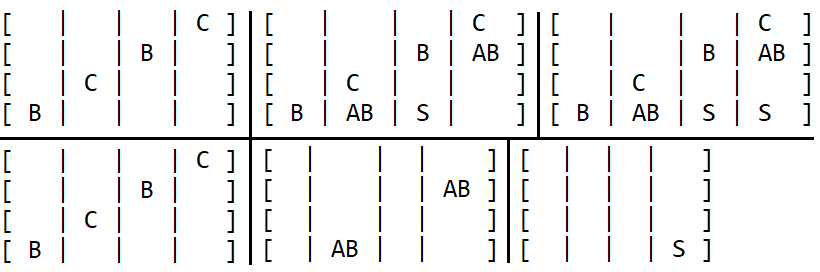
\includegraphics[width=0.9\textwidth]{obrazky-figures/comparisionOfTables.png}
	\caption{Porovnanie vypĺňania obsahov tabuliek algoritmov CYK. Prvý riadok obsahuje tabuľky pre algoritmus CYK pre bezkontextové gramatiky. Druhý obsahuje tabuľky modifikácie algoritmu CYK pre E0L systémy.}
	\label{compareTables}
\end{figure}

%---------------------------------------------------------------------------------
\subsection*{ET0L systémy}
Pri tejto modifikácii algoritmu \textit{CYK} budeme vychádzať z už popísanej modifikácie pre E0L systémy (viď \ref{EOL parsing}). Nad modifikáciou pre E0L systémy zapracovať spracovanie pre viaceré tabuľky pravidiel, ktorými sa vyznačujú ET0L systémy.

Tabuľky, alebo ináč povedané množiny pravidiel, rozvetvujú spracovanie syntaktickou analýzou. Pri každom kroku môže byť použitá ľubovoľná tabuľka. To znamená, že algoritmus sa musí nutne rozvetvovať kvôli rôznym postupnostiam výberu tabuliek. Musia byť skontrolované všetky kombinácie výberu tabuliek v jednotlivých krokoch. 

O tomto probléme sa dá povedať, že je to \textit{prehľadávanie stavového priestoru}, ktorým sa zaoberá umelá inteligencia. V skratke ide o to, že musíme nájsť takú postupnosť operátorov, aby sme sa dopracovali ku konečnému stavu. Operátory v našom prípade môžeme chápať ako tabuľku pravidiel a konečný stav je tabuľka CYK, ktorá na pozícii [1, n] obsahuje počiatočný symbol. Teda úspešné ukončenie algoritmu.

\subsubsection*{Backtracking}
Jednou z metód riešenia problému prehľadávania stavového priestoru je práve backtracking. Jedná sa o neinformovanú metódu, nemá teda žiaden spôsob ako jednotlivé stavy ohodnotiť \cite{IZU}. To nám pre túto modifikáciu algoritmu CYK vyhovuje, pretože by bolo obtiažne, ak vôbec možné, vhodne ohodnotiť stav tabuľky CYK.

Backtracking namiesto expanzie vybraného uzlu(stavu) vygeneruje iba jedného následníka. Expanzia uzlu by v našom prípade znamenala aplikáciu všetkých tabuliek na~aktuálnu tabuľku CYK a získanie $n$ nových tabuliek CYK, kde $n$ je počet tabuliek pravidiel.

Pri nájdení nevyhovujúceho stavu sa metóda backtrackingu vráti na predchádzajúci stav a vygeneruje sa ďalší nasledovník. Pokiaľ sa už žiaden nový nasledovník vygenerovať nedá, metóda sa vracia o krok späť, pokiaľ je to možné \cite{IZU}.


\subsection*{Popis fungovania}
Backtracking je docielený rekurzívnym spustením ďalšieho kroku pre každú existujúcu tabuľku. Na začiatku kroku je nastavená tabuľka, ktorá sa v danom kroku bude používať. Na konci kroku sa znova rekurzívne spustia kroky pre všetky existujúce tabuľky pravidiel. Keďže prvý krok nemôže byť spustený predchádzajúcim, sú všetky prvé kroky spustené po naplnení diagonály neterminálmi. Veľmi dôležité je aj samotné napĺňanie diagonály neterminálmi. Keďže existuje viacero tabuliek pravidiel, je potrebné naplniť diagonálu pomocou každej z nich. Tento popis je podrobne popísaný pomocou pseudokódu \ref{CYKET0L}.

Týmto spôsobom získavame backtracking nad aplikáciou všetkých možných kombinácii tabuliek pravidiel v jednotlivých krokoch.

\begin{algorithm}
\caption{Cocke-Younger-Kasami algoritmus syntaktickej analýzy pre ET0L systémy}
\label{CYKET0L}

\textbf{Input}
\setlist{nolistsep}
\begin{itemize}[noitemsep]
    \item ET0L system, \(E = (\Sigma, T, P^T, w_o))\) in normal form \ref{E0LNormalForm}
    \item \(w = a_1a_2...a_n\)  where  \(a_i \in {}_E\Delta, 1 \leq i \leq n \), for some \(n \geq 1\).
\end{itemize}
\textbf{Output} 
\begin{itemize}[noitemsep]
    \item \textbf{ACCEPT} if \(w \in L(G)\)
    \item \textbf{REJECT} if \(w\notin L(G)\)
\end{itemize}
\textbf{Method}
\begin{algorithmic}
\For{$\forall P \in P^T$}
\State $ CYK[i,j] = \varnothing$ for $1 \leq i \leq j \leq n $

\For{i = i \textbf{to} $n$}
    \If{$ A \rightarrow a_i \in P $}
        \State $add\ A\ to\ CYK[i,i]$
    \EndIf
\EndFor
\For{$\forall X \in {}_ET$}
\State \Call{CYKCycle}{CYK, P, $\varnothing$}
\EndFor
\EndFor

\State \textbf{REJECT}
\\
\Function{CYKCycle}{CYK, P, history}
\State $ CYKNext[i,j] = \varnothing$ for $1 \leq i \leq j \leq n $
\State $ empty\ is\ set\ of\ terminals,\ \forall A \in empty, A \Rightarrow^* \epsilon\ and\ A \in \Sigma / T$

\Repeat

\If{$ A \in CYK[i,j], \alpha \rightarrow A \in P $ for some $A, \alpha \in \Sigma$}
\State
\State $add\ \alpha\ to\ CYKNext[i,j]$
\EndIf

\If{$ B \in CYK[i,j], C \in empty, A \rightarrow BC \lor A \rightarrow CB \in P $ for some $A,B,C \in \Sigma / T$ \phantom{xxxxx}}
\State $add\ A\ to\ CYKNext[i,j]$
\EndIf

\If{$ B \in CYK[i,j], C \in CYK[j+1,k], A \rightarrow BC \in P $ for some $A,B,C \in \Sigma/T$}
\State $add\ A\ to\ CYKNext[i,k]$
\EndIf
\Until{no changes}

\If{$(CYKNext, empty) \in history$}
    \State \textbf{return}
\Else
    \State $add\ (CYKNext, empty)\ to\ history$
\EndIf

\If{No new reduction in this step}
\State \Return
\EndIf
\If{$ S \in CYKNext[1,n] $}
    \State \textbf{ACCEPT}
\Else
    \State $ CYK = CYKNext$
    \For{$\forall R \in P^T$}
        \State \Call{CYKCyklus}{CYK, R, history}
    \EndFor
\EndIf


\EndFunction

\end{algorithmic}
\end{algorithm}

\section{Algoritmus zhora-dole pre ET0L systémy}
\label{top-downET0L}
Prístup syntaktickej analýzy zhora-dole predstavuje opačný prístup ako zdola-hore, ktorý je využívaný v algoritme CYK a aj v jeho navrhovaných modifikáciách.

Nevýhodou tohto prístupu je väčšia časová zložitosť, nakoľko v najhoršom prípade musíme vygenerovať všetky možné slová o danej dĺžke. To však predstavuje aj výhodu, pretože je možné tento algoritmus použiť na všetky možné slová o danej dĺžke. Ďalšou výhodou je, že pravidlá môžu byť v ľubovoľnom tvare.

\subsection*{Riešenie nedeterminizmu a paralelizmu}
Jedným z dvoch hlavných problémov pre tento druh syntaktickej analýzy sú nedeterministické pravidlá, to znamená, že jeden symbol sa vyskytuje na ľavej strane viacerých pravidiel. Ináč povedané, existuje možnosť, že sa môže prepísať na viacero rôznych reťazcov. Riešením tohto problému je rekurzia. Pri každej aplikácii pravidla sa použitím rekurzie zaistí, že sa vygenerovali všetky možnosti aplikácii rôznych pravidiel pre~prepisovaný symbol.

Druhým problémom je zaistiť paralelizmus prepisovania. Problém je to preto, lebo tento paralelizmus potrebujeme docieliť pomocou sekvencie akcií. Musíme teda napodobniť paralelizmus sekvenčne. To je dosiahnuté zavedením indexu ukazujúceho na symbol, ktorý má byť prepísaný ako ďalší. Pokiaľ index neukazuje na začiatok slova, tak na toto slovo neboli aplikované všetky potrebné pravidlá, derivačný krok teda stále prebieha.

\subsection*{Popis fungovania}
Máme určené počiatočné slovo, na ktoré budú aplikované derivačné kroky. Na začiatku je index nastavený na 0 (v rámci tohto algoritmu uvažujeme indexovanie od 0), čiže na index prvého symbolu slova.

Existuje funkcia, ktorá slúži na aplikáciu individuálnych pravidiel. Keďže sú ET0L systémy plne paralelné, musia sa aplikovať pravidlá na všetky symboly slova súčasne, nejde o~kompletný derivačný krok. Funkcia ako parametre prijíma reťazec, index a aktuálnu tabuľku pravidiel (keďže sa jedná o ET0L systémy).

Táto funkcia na aplikáciu pravidiel aplikuje z tabuľky symbolov všetky existujúce pravidlá na symbol, na ktorý ukazuje index. Tento index je prepočítaný podľa pravidla, ktoré sa aplikovalo. Zvýši (posunie) sa o dĺžku pravej strany aplikovaného pravidla. Ukazuje na ďalší symbol pôvodného slova. Pokiaľ bolo pravidlo aplikované na posledný symbol, index sa vracia na začiatok slova, teda na nulu.

Po tom ako funkcia aplikuje pravidlo a prepočíta index, rekurzívne zavolá sama seba s~týmito novými hodnotami. V prípade, že je nový index nulový, znamená to, že bol dokončený celý derivačný krok. Preto funkcia navyše rekurzívne zavolá samú seba pre každú tabuľku pravidiel, ktorú daný ET0L systém obsahuje.

Samozrejme sa na začiatku tejto funkcie musia kontrolovať slová, ktoré funkcia prijala ako parameter. To slúži ako ukončovacia podmienka tejto rekurzie. Jednou je, že sme dosiahli slovo, ktoré kontrolujeme. V tom prípade algoritmus končí \textbf{úspechom}. Druhou je, že prijaté slovo je dlhšie, než dĺžka kontrolovaného slova. Ak algoritmus skončí bez toho, aby bolo vygenerované vyhľadávané slovo, algoritmus končí neúspechom.

Tento algoritmus je v ekvivalentnej forme zapísaný pomocou pseudokódu \ref{topDownET0L}.

\subsubsection*{Generátor slov}
Pokiaľ algoritmus mierne modifikujeme, je pomocou neho možné vygenerovať všetky možné slová o istej maximálnej dĺžke z jazyka, ktorý je generovaný daným ET0L systémom.

Pokiaľ je počas syntaktickej analýzy vygenerované slovo, ktoré obsahuje len neterminály a má správnu dĺžku, pridá sa do množiny vygenerovaných slov. Je nutné zrušiť kontrolu úspešnosti. Tá by nastala v prípade, že slovo vygenerované syntaktickou analýzou je rovnaké ako kontrolované slovo. Pokiaľ by táto kontrola nebola zrušená, neboli by vygenerované žiadne slová, ktoré by boli vygenerované po kontrolovanom slove.


\begin{algorithm}
\caption{Algoritmus syntaktickej analýzy ET0L systémov zhoda-dole}
\label{topDownET0L}

\textbf{Input}
\setlist{nolistsep}
\begin{itemize}[noitemsep]
    \item ET0L system, \(E = ({}_E\Sigma, {}_ET)\)
    \item \(w = a_1a_2...a_n\)  where  \(a_i \in {}_E\Delta, 1 \leq i \leq n \), for some \(n \geq 1\).
\end{itemize}
\textbf{Output} 
\begin{itemize}[noitemsep]
    \item \textbf{ACCEPT} if \(w \in L(G)\)
    \item \textbf{REJECT} if \(w\notin L(G)\)
\end{itemize}
\textbf{Method}
\begin{algorithmic}
\For{$\forall R \in {}_ET$}
    \State \Call{applyRule}{$w_o, 0, R$}
\EndFor

\State \textbf{REJECT}
\Comment{No recursive call of ApplyRule accepted}
\\
\Function{applyRule}{word, index, ruleSet}
\If{$word = w$}
    \State $ACCEPT$
\EndIf

\If{$|word| > |w|$}
    \State \Return
\EndIf

\For{$\forall R \in ruleSet$ where $word[index] \to x, x \in {}_\Sigma$}
    \State $newWord$ = replace $word[index]$ with $x$ in $word$
    \State $newIndex$ = $index + |x|) \mod |newWord|$
    \If{$newIndex == 0$}
        \For{$\forall R \in {}_ET$}
        \Comment{derivation step complete, use all tables recursively}
            \State \Call{applyRule}{newWord, newIndex, R}
        \EndFor
        \State \Call{applyRule}{newWord, newIndex, ruleSet}
        \Comment{derivation step is not complete}
    \EndIf
\EndFor
\EndFunction
    
\end{algorithmic}
\end{algorithm}

\subsection*{Verzia pre E0L systémy}
Tento algoritmus je možné aplikovať aj pre E0L systémy. Tie sú vlastne špeciálnym typom ET0L systémov, ktoré majú len jednu tabuľku. Preto je tento algoritmus použiteľný pre~E0L systémy.

\subsection*{Verzia pre bezkontextové gramatiky}
Algoritmus je možné upraviť pre bezkontextovú gramatiku nasledovne. Odstráni sa indexácia v rámci slova. Rekurzívne volanie funkcie sa vykoná pre každý symbol v slove. Takto získame algoritmus pre generovanie slov bezkontextových gramatík.

\subsection*{Nedostatok návrhu}
Navrhnutý algoritmus obsahuje nedostatok pri práci s prázdnymi prepisovacími pravidlami. Ten zamieta vygenerované slová, ktoré sú dlhšie než kontrolované slovo. Aplikáciou prázdnych prepisovacích pravidiel je však možné získať 
z dlhšieho slova kratšie.

Možným riešením je využitie množiny $empty$ podobne ako pri modifikáciách algoritmu CYK. Do dĺžky slova by neboli započítané prvky tejto množiny pretože by mohli byť zmazané. Toto riešenie však nie je možné použiť. Ako príklad uvažujme prepisovacie pravidlá $S \to A$, $A \to AA$, $A \to a$, $A \to \epsilon$. Ľubovoľne dlhý reťazec o dĺžke $n$ neterminálov $A$ je možné jedným paralelným derivačným krokom získať reťazec o dĺžke $\leq n$. Preto by mohli byť pomocou algoritmu generované nekonečné dlhé slová.

%=============================================================================================
\chapter{Implementácia}
\label{implementation}

V predchádzajúcej kapitole boli predstavené a popísané dve metódy syntaktickej analýzy pre ET0L systémy. Prvá z nich pracuje na princípe syntaktickej analýzy zdola-hore (viď \ref{analysysTypes}), teda z pôvodného slova sa spätne redukciou pravidiel vracia k počiatočnému symbolu. Táto metóda vychádza z algoritmu Cocke-Younger-Kasami a pomocou jeho modifikácie získavame algoritmus, ktorý funguje pre syntaktickú analýzu ET0L systémov.

Druhou variantou je algoritmus na princípe zhora-dole, snaží sa teda vygenerovať dané slovo aplikáciou pravidiel na počiatočné slovo.

\section{Návrh implementácie}
Tieto metódy syntaktickej analýzy je potrebné implementovať v rámci aplikácie. Ako aplikáciu som zvolil konzolové rozhranie, ktoré spúšťa a interaguje s jednotlivými algoritmami. Jedná sa o rozhranie, pomocou ktorého je možné vybrať konkrétny algoritmus. Pomocou tohto algoritmu sa vykoná syntaktická analýza.

Keďže sa jedná o konzolovú aplikáciu, všetky potrebné voľby a parametre sú špecifikované pomocou parametrov predaných cez konzolové rozhranie.

Metódy syntaktickej analýzy, ktoré boli špecifikované pre ET0L systémy, boli vytvorené aj pre bezkontextové gramatiky a E0L systémy, pretože na seba naväzujú. Každý tento algoritmus je implementovaný pomocou samostatného skriptu.

\section{Implementačný jazyk}
Pred samotnou implementáciou bolo potrebné zvoliť vhodnú platformu implementácie.

Zvolil som programovací jazyk \textbf{Python} vo verzii 3.7 . Jedná sa o vysokoúrovňový objektovo orientovaný programovací jazyk. Poskytuje vysokú mieru abstrakcie nad jednotlivými konštruktmi ktoré obsahuje spoločne s bohatou štandardnou knižnicou. Pomocou jazyka Python preto možný rýchly vývoj. Vďaka týmto pozitívam sa hodí na~implementáciu algoritmov definovaných v tejto práci.

Hlavnou nevýhodou jazyka Python je, že sa jedná o interpretovaný jazyk. Na jeho spustenia teda musíme mať nainštalovaný interpret. Vo všeobecnosti sú interpretované jazyky pomalšie, čo platí aj pre Python. Pre túto prácu to však nepredstavuje problém.


\section{Štruktúra aplikácie}
Každá implementácia jednotlivých algoritmov je tvorená triedou v samostatnom súbore. Keďže boli navrhnuté dve metódy syntaktickej analýzy a je implementovaná verzia pre~bezkontextové gramatiky, E0L a ET0L systémy, existuje 6 tried syntaktických analýz.

Pre prácu algoritmov syntaktickej analýzy je potrebný vstupný formálny model, teda gramatika alebo L-systém. Najdôležitejšou časťou tohto vstupného modelu sú prepisovacie pravidlá. Vďaka forme týchto pravidiel a ich potencionálnej dĺžke bola vytvorená trieda, ktorá tieto pravidlá získava zo súboru. Existujú dve implementácie tejto triedy. Pri ET0L systémoch je potrebné rozdeliť pravidlá do viacerých tabuliek a preto je potrebné vhodne upraviť implementáciu.

Užívateľské rozhranie aplikácie tvorí skript, ktorý pomocou konzolového rozhrania prijíma od užívateľa potrebné informácie pre spustenie jednotlivých syntaktických analýz.

\section{Rozhranie aplikácie}
Ako rozhranie pre interakciu užívateľa s jednotlivými algoritmami syntaktickej analýzy bolo zvolené konzolové rozhranie. Pomocou konzolových parametrov užívateľ programu poskytuje informácie, ktoré sú potrebné k správnemu fungovaniu. 

Konzolové parametre sú: 

\begin{itemize}
    \item[] -h, (help) vypísanie nápovedy pre správne používanie aplikácie
    \item[] -C | E | T , výber verzie algoritmu pre bezkontextové gramatiky, E0L alebo ET0L systémy v tomto poradí
    \item[] -r <rules>, špecifikovanie súboru v ktorom sa nachádzajú prepisovacie pravidlá. Forma pravidiel je podrobne popísaná v časti \ref{ruleFormat}
    \item[] -w <word>, špecifikovanie slova, ktoré má byť spracované pomocou syntaktickej analýzy
    \item[] --top-down, použitie algoritmov založených na princípe zhora dole
    \item[] --start-word <axiom>, definovanie $axiomu$ pre algoritmus na princípe zhora dole. Východzia hodnota je \uv{S}
    
\end{itemize}

\section{Načítanie prepisovacích pravidiel}
Každá implementácia algoritmov syntaktickej analýzy potrebuje mať nejakým spôsobom definované prepisovacie pravidlá. Či už to je napevno naprogramované v kóde, alebo sú tieto pravidlá načítané dynamicky.

V tejto aplikácii sa pravidlá načítavajú zo špecifikovaného súboru obsahujúceho tieto pravidlá. Je potrebné vhodne načítať tabuľky pravidiel pre ET0L systémy. Preto existujú dve implementácie triedy \textbf{\texttt{RuleReader}}, ktorá implementuje načítanie pravidiel zo súboru.

\subsection*{Formát súboru s pravidlami}
\label{ruleFormat}
Prepisovacie pravidlá, ktoré potrebujú algoritmy syntaktickej analýzy, musia byť uložené v~samostatnom súbore. Tento súbor môže mať ľubovoľný názov, ktorý sa predáva aplikačnému rozhraniu.

Každé pravidlo musí byť na samostatnom riadku a spĺňať nasledovný formát:
\[\text{s--->s${}^+$ alebo s--->-}, \quad\quad \text{kde s je ľubovoľné písmeno}\]

To znamená, že prepisovaný znak, teda písmeno na ľavej strane, môže byť len jedno, keďže všetky navrhnuté algoritmy sú bezkontextové. Na pravej strane pravidla, teda reťazec, ktorým sa prepíše znak na ľavej strane, môže pozostávať z jedného alebo viacerých písmen, veľkých aj malých. Ľavé a pravé strany pravidiel sú od seba oddelené znakmi \uv{-} a \uv{>}, ktoré spoločne tvoria šípku.

Pri vytváraní objektu triedy \texttt{RuleReader} je potrebné konštruktoru predať názov súboru, z ktorého sa majú pravidlá načítať.

\subsubsection*{Oddelenie tabuliek pravidiel pre ET0L systémy}
ET0L systémy umožňujú používanie viacerých množín prepisovacích pravidiel, ktoré sa nazývajú tabuľky. Preto je potrebné tieto tabuľky vo vstupnom súbore s pravidlami vymedziť. Jednotlivé tabuľky sú od seba oddelené pomocou znaku \textbf{\uv{\#}} na samostatnom riadku.

\subsubsection*{Kontrola formátu pravidiel}
Pri načítaní pravidiel zo súboru sú tvary pravidiel kontrolované pomocou \textit{RegEx}-ov, čo je implementácia regulárnych výrazov popísaných v časti \ref{regularExpression}.

V prípade používania algoritmov založených na algoritme Cocke-Younger-Kasami (ďalej len CYK), pravidlá musia byť v správnej normálovej forme (\ref{E0LNormalForm}). Táto podmienka je taktiež kontrolovaná pomocou \textit{RegEx-ov}.
\\\\
Pri načítaní vstupného súboru sa ignorujú netlačiteľné (white-space) znaky.

\subsection*{Reprezentácia prepisovacích pravidiel}
Pre vnútornú reprezentáciu prepisovacích pravidiel sa používa dátová štruktúra slovník (anglicky dictionary), ktorá sa taktiež nazýva hašovacia tabuľka (anglicky hash-table). Táto štruktúra umožňuje zaviesť indexáciu pomocou vlastných kľúčov, ktoré slúžia na~indexovanie. V implementácii sa ako kľúče využívajú ľavé strany pravidiel, teda symboly, ktoré sa majú prepísať. Hlavnou výhodou tejto dátovej štruktúry je rýchly prístup k dátam a jednoduchosť používania.

Slovník pre každý kľúč, teda ľavú stranu pravidla, uchováva zoznam pravých strán pravidiel, ktoré predstavujú reťazce, ktorými sa môže daná ľavá strana pravidla prepísať. Pravé strany pravidiel pre konkrétnu ľavú stranu musia byť ukladané v zozname, keďže množina pravidiel nemusí byť deterministická a môže tak obsahovať viacero pravých strán pre tú istú ľavú stranu pravidiel.

Pre získanie pravidiel slúži metóda triedy \texttt{RuleReader} nazvaná \texttt{getRulesDictionary}, ktorá prijíma parameter rozhodujúci o tom, či majú byť pravidlá kontrolované pre vhodnú normálovú formu.

Implementácia triedy \texttt{RuleReader} pre jednu množinu pomocou metódy \texttt{getRulesDictionary} má ako návratovú hodnotu slovník pravidiel. V prípade implementácie pre viacero tabuliek pravidiel používanej pre ET0L systémy, je návratová hodnota zoznam slovníkov pravidiel.

\section{Syntaktická analýza}
Oba spôsoby syntaktickej analýzy navrhnutej v kapitole \ref{syntax} sú implementované ~bezkontextové gramatiky, E0L a ET0L systémy. Jednotlivé implementácie sú tvorené triedou a metódou \texttt{parse}, ktorá prijíma ako parameter reťazec určený pre syntaktickú analýzu.

\subsubsection*{Reprezentácia formálnych modelov}
Modely, s ktorými pri syntaktickej analýze pracujeme sú bezkontextové gramatiky, E0L a ET0L systémy. Síce ide o tri rozdielne formálne modely, sú ale definované rovnakými základnými vlastnosťami. Jedná sa o abecedu terminálov a neterminálov, prepisovacie pravidlá a počiatočný symbol, prípadne slovo.

Definícia prepisovacích pravidiel už bola popísaná skôr v tejto kapitole. Abeceda terminálov a neterminálov nie je definovaná explicitne. Nie je to potrebné, stačí, že sú použité v rámci prepisovacích pravidiel. Predpokladá sa, že veľké písmená reprezentujú neterminály a malé písmená zasa terminály. Takáto reprezentácia je v rámci teoretickej informatiky bežne používaná. $\epsilon$ na pravej strane prepisovacieho pravidla je reprezentovaný pomocou pomlčky (\uv{-}).

Bezkontextové gramatiky majú vo svojej definícii počiatočný symbol, E0L a ET0L systémy takzvaný \textit{axiom}, počiatočné slovo. Všetky implementácie týchto formálnych modelov založené na algoritme CYK predpokladajú ako počiatočný symbol alebo axiom neterminál \uv{S}. Implementácie algoritmov založených na princípe zhora-dole pre E0L a ET0L sytémy ako axiom implicitne používajú neterminál \uv{S}. Pomocou parametra \texttt{startWord} funkcie \texttt{parse} je však možné použiť ľubovoľný reťazec obsahujúci len terminály a neterminály. To však neplatí pre verziu pre bezkontextové gramatiky. Tam je počiatočný symbol vždy \uv{S}.


\subsubsection{Obmedzenia rekurzie}
Algoritmy syntaktických analýz pre ET0L systém využívajú vo svojom návrhu rekurziu. Algoritmy sú však výpočetne náročný a pri použití rekurzie mal príliš veľkú hĺbku zanorenia. To znamená, že funkcia príliš veľa krát zavolala sama seba bez toho, aby sa navrátila z tohto vnorenia. Preto pri využití rekurzie nastali dva problémy. Prvým je, že algoritmy boli príliš pomalé. Druhým je obmedzenie jazyka Python na maximálnu hĺbku rekurzie, ktorá bola prekročená. Dôsledkom toho bol program zastavený a systémom automaticky ukončený.

\subsubsection{Prevod rekurzívnej funkcie do iteratívnej formy}
Riešením problémov spojených s rekurziou je prevod rekurzívnej funkcie na iteratívnu. Pre~parametre takejto funkcie sa vytvoria zásobníky a vložia sa do nich počiatočné hodnoty.  Obsah funkcie sa zabalí do cyklu, ktorý sa vykonáva, kým nie sú zásobníky prázdne. Na~začiatku cyklu sa vyberú hodnoty z vrcholov zásobníkov. Rekurzívne volanie funkcie sa nahradí vložením hodnôt parametrov do zásobníkov. Vďaka tomu je rekurzívna funkcia konvertovaná na iteratívnu.

\subsection{Syntaktická analýza založená na Cocke-Younger-Kasami algoritme}


Triedy \texttt{CFGParserCYK}, \texttt{E0LParserCYK}, \texttt{ET0LParserCYK} sú implementácie navrhnutých algoritmov pre syntaktickú analýzu v kapitole \ref{syntax} pomocou modifikácie algoritmu Cocke-Younger-Kasami pre bezkontextové gramatiky (viď \ref{CYK}). Pseudokód fungovania týchto implementovaných tried je popísaný v algoritmoch \ref{CYKBKG} pre bezkontextové gramatiky implementovaný v triede \texttt{CFGParserCYK}, \ref{CYKE0L} pre E0L systémy implementovaný v triede \texttt{ET0LParserCYK} a \ref{CYKET0L} pre E0L systémy implementovaný v triede \texttt{ET0LParserCYK}.


\subsubsection*{Vnútorná reprezentácia tabuliek algoritmu CYK}
Tieto tabuľky slúžia pre uchovávanie stavu symbolov počas algoritmu CYK. Jedná sa o~dvojrozmerné pole symbolov. Dátový typ jednotlivých položiek tabuľky je \texttt{množina}, v~jazyku Python reprezentovaná pomocou \texttt{set()}. Tento dátový typ je nezoradený a vždy obsahuje len unikátne hodnoty. To je výhodné, nakoľko duplicitné hodnoty sú v týchto tabuľkách zbytočné. Vďaka využitiu tohto dátového typu nie je potrebné túto duplicitu riešiť.

\subsubsection*{Formátovanie výpisu tabuliek algoritmu CYK}
Na konci každého kroku týchto algoritmov je do konzoly vypísaný aktuálny stav tabuľky CYK. Funkcia \texttt{print()}, ktorá v jazyku Python slúži na výpis do konzoly, dokáže spracovať aj dvojrozmerné polia, akým sú aj tabuľky používané algoritmom CYK. Tento výpis však nie je užívateľsky prívetivý a zle sa v ňom orientuje.

Každá trieda obsahuje funkciu na výpis týchto tabuliek, nazvanú \texttt{printTable}. Tá invertuje tabuľku podľa osy Y, takže index $[0, 0]$ je v ľavom spodnom rohu. Taktiež zabezpečí, že šírka stĺpca je určená podľa najdlhšej množiny symbolov v danom stĺpci. Vďaka tomu sú tabuľky vypísané do konzoly pre užívateľa ľahko pochopiteľné. Príklad výpisu tabuľky je možné vidieť na obrázku \ref{tableExample}.

\begin{figure}[hbt]
	\centering
	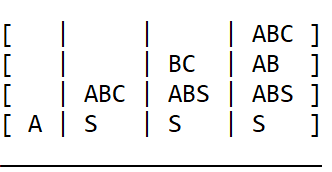
\includegraphics[width=0.4\textwidth]{obrazky-figures/exampleTable.png}
	\caption{Ukážka výpisu tabuľky algoritmu Cocke-Younger-Kasami. Formátovanie šírky stĺpcov je určené podľa najširšej bunky daného stĺpca.}
	\label{tableExample}
\end{figure}

\subsubsection*{Výstup algoritmu}
Triedy \texttt{CFGParserCYK} a \texttt{E0LParserCYK} priebežne vypisujú aktuálnu tabuľku $CYK$ na~štandardný výstup. To však nie je vhodné pre triedu \texttt{ET0LParserCYK}, nakoľko by bol tento výpis kvôli prehľadávaniu správnej kombinácie tabuliek neprehľadný. Vypíše sa len postupnosť tabuliek, ktorá viedla k~úspešnosti syntaktickej analýzy. Ak analýza úspešná nebola, nevypíše sa nič. Metóda \texttt{parse} pri úspechu syntaktickej analýzy vracia hodnotu \texttt{True}, ináč \texttt{False}. To platí pre všetky triedy.

Pred vypisovaním samotných tabuliek je vypísané slovo, ktoré bude syntaktická analýza spracovávať.

\subsubsection*{Nedostatky implementovaného algoritmu}
Pri implementácii bol objavený nedostatok tohto algoritmu pri používaní komplikovaných prepisovacích pravidiel, ktoré obsahujú aj prázdne prepisovacie pravidlá. Implementácia verzie tohto algoritmu pre ET0L systémy bola pomalá pre správne aj nesprávne slová. V niektorých prípadoch trvala jednotky sekúnd. Jednoduchou zmenou vyberania hodnôt zo zásobníkov bolo možne tento problém odstrániť aspoň pre správne slová. Hodnoty sa nevyberajú z vrcholu zásobníku ale z jeho spodku. Tým sa zásobník mení na frontu. Problém s rýchlosťou pre neplatné slová zostáva.

\subsection{Syntaktická analýza zhora-dole}
\label{topDownImplementation}
Implementované algoritmy pre jednotlivé formálne modely sú popísané v časti \ref{top-downET0L}. Trieda \texttt{TopDownCFGParser} je implementáciou verzie algoritmu syntaktickej analýzy pre~bezkontextové gramatiky, \texttt{TopDownE0LParser} pre E0L systémy a \texttt{TopDownET0LParser} pre ET0L systémy.


\subsubsection*{Generovanie slov}
Jednoduchou úpravou tejto syntaktickej analýzy je možné vygenerovať všetky slová patriace do jazyka, ktorých dĺžka je menšia alebo rovná $n$, pričom $n \geq 1$. Pri nedodržaní tejto podmienky nebude nikdy vygenerované žiadne slovo.

Metóda \texttt{generateValidWords} slúži na vygenerovanie týchto slov. Tá interne využíva rovnakú metódu, ako metóda syntaktickej analýzy \texttt{parse}. Ak je počas generácie získané platné slovo, pridá sa do množiny \texttt{generatedWords}, ktorá obsahuje vygenerované slová. Vygenerované slová môžu byť použité pre testovanie syntaktickej analýzy založenej na~algoritme CYK.

Pomocou metódy \texttt{generateAllCombinations} vygeneruje všetky možné kombinácie terminálov, ktorých dĺžka je menšia alebo rovná $n$. Vygenerované kombinácie môžu byť rozdelené na dva disjunktné množiny. Jednou sú slová patriace do generovaného jazyka a~druhou sú tie, ktoré do neho nepatria.

Pokiaľ je vykonaný rozdiel množín, kde od všetkých kombinácii terminálov odčítame reťazce generované jazykom, získame množinu slov ktoré do generovaného jazyka nepatria. Takáto množina má využitie pri testovaní.

\subsubsection{Výstup algoritmu}
Metóda \texttt{parse} pri úspechu syntaktickej analýzy vracia hodnotu \texttt{True}, ináč \texttt{False}. To platí pre všetky triedy.

Metódy \texttt{generateValidWords} a \texttt{generateAllCombinations} vracajú množiny.

%=============================================================================================
\chapter{Testovanie}
\label{testovanie}
Na testovanie softvéru sa niekedy vynakladá viac zdrojov než na samotnú implementáciu. Platí to hlavne v prípade, kedy chyba daného softvéru môže spôsobiť veľké škody, napríklad pád lietadla.

Testovaniu sa v rámci tejto práce nebudeme venovať do hĺbky, nakoľko sa jedná o veľmi komplexnú tematiku. Rozdelenie druhov testov môže byť niekedy neurčité, pojmy sa môžu prekrývať, alebo môžu byť úplne zamenené.

V rámci tejto práce testujeme funkčnosť tried syntaktických analýz ako celkov.

\section{Rozhranie testov}
Skript pre samotné vykonanie testov je implementovaný v súbore \texttt{parserTest.py}. Nie je využívaná žiadna knižnica poťažmo framework pre testovanie. To prebieha vytváraním objektov tried syntaktických analýz a kontrolovaním výsledku spustenia funkcie \texttt{parse}.


\subsection*{Testovacie vstupy}
Pri spúšťaní syntaktických analýz je potrebné im predať isté vstupné hodnoty. Konkrétne súbor s prepisovacími pravidlami a slovo, ktoré sa má kontrolovať.

Za účelom tohto testovania bol vytvorený samostatný súbor s prepisovacími pravidlami, ktorý je v rámci testovania používaný. Tento súbor s prepisovacími pravidlami obsahuje všetky možnosti vlastností prepisovacích pravidiel, ktoré sa v rámci syntaktickej analýzy chovajú odlišne.

Vstupné slová sú generované syntaktickou analýzou zhora dole. Triedy týchto analýz obsahujú metódu \texttt{generate}, ktorá vracia dvojicu \texttt{touple} množín. Prvá množina obsahuje všetky slová patriace do generovaného jazyka o maximálnej dĺžke $n$, pričom $n$ je parameter metódy \texttt{generate}. Druhá množina obsahuje všetky platné slová o dĺžke $n$, ktoré však nepatria do generovaného jazyka.

Vďaka tomu, že generujeme aj všetky slová, ktoré nepatria do generovaného jazyka, sú vylúčené takzvané \textit{false positives}. Tento výraz znamená, že test prebehol úspešne aj keď nemal. Ako názornú ukážku uvažujme algoritmus syntaktickej analýzy, ktorý prijme všetky slová, aj keď nepatria do generovaného jazyka. Pri jeho testovaní len pomocou slov patriacich do generovaného jazyka by testy mali 100\%-nú úspešnosť. Pokiaľ by boli testované slová, ktoré majú byť odmietnuté, úspešnosť testov by bola 0\%. Vďaka týmto testom by sme zistili, že algoritmus je nefunkčný.

\subsection{Zohľadnenie nedostatkov algoritmov}
Testované syntaktické analýzy obsahujú dva problémy. Modifikácia algoritmu CYK pre~ET0L systémy je pomalá pri existencii prázdnych prepisovacích pravidiel a následnej kontrole neplatných slov. Algoritmy založené na princípe zhora-dole zasa odmietajú niektoré slová, ktoré by mohli byť aplikáciou prepisovacích pravidiel skrátene na požadovanú dĺžku a následne prijaté. To by znamenalo, že by boli pri generovaní vstupných slov označené ako~neplatné.

Pri testovaní nesprávnych slov sú použité také prepisovacie pravidlá, ktoré neobsahujú prázdne prepisovacie pravidlá.

\subsection*{Testované analyzátory}
Generácia vstupných slov pre testovanie prebieha pomocou syntaktických analýz zhora-dole. Táto funkcionalita je popísaná v časti \ref{topDownImplementation}. Preto nie je dôvod pomocou týchto vstupov tieto analýzy testovať. Testované sú len syntaktické analyzátory založené na algoritme Cocke-Younger-Kasami.

Vyplýva však otázka, ako si môžeme byť istý, že syntaktická analýza zhora-dole funguje správne. Táto syntaktická analýza je nepriamo testovaná pomocou testov syntaktickej analýzy CYK. Pokiaľ oba tieto druhy syntaktickej analýzy prijímajú a odmietajú rovnakú množinu slov pre konkrétny formálny model, je nepravdepodobné, že sú obe chybné.

\subsection*{Výstup testovania}
Po spustení testov sa všeobecne očakáva istý výstup, ktorý informuje o úspešnosti jednotlivých testov. V prípade neúspešnosti niektorých, prípadne všetkých testov, musí byť z výstupu jasné, ktoré testy prebehli neúspešne. Dôležitou informáciou je taktiež koľko testov z celkového počtu spustených testov prebehlo úspešne.

Pri testovaní v rámci tejto práce je výstup vypísaný na štandardný výstup. Pre každú testovanú syntaktickú analýzu sú vždy vypísané počty úspešne spracovaných slov, ktoré patria do generovaného jazyka. Taktiež sú vypísané počty úspešne spracovaných slov, ktoré nepatria do generovaného jazyka.

V prípade, že syntaktická analýza nesprávne spracuje vstupné slovo, je táto informácia vypísaná na štandardný vstup spolu s daným slovom.

Príklad tohto výstupu je možné vidieť na obrázku \ref{testOutput}. Pri tomto testovaní bola pre~názornosť do testovacieho skriptu schválne zavedená chyba.

\begin{figure}[hbt]
	\centering
	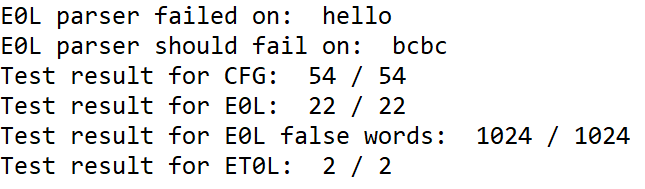
\includegraphics[width=0.6\textwidth]{obrazky-figures/testOutput.png}
	\caption{Príklad výstupu testovacieho skriptu. Do testovacieho skriptu bola zámerne zavedená chyba. Syntaktická analýza pre E0L systémy odmietla slovo \texttt{hello}, ktoré mala podľa testov prijať. Naopak, prijala slovo \texttt{bcbc}, ktoré mala podľa testov odmietnuť.}
	\label{testOutput}
\end{figure}

\subsubsection*{Blokovanie štandardného vstupu}
Syntaktická analýza založená na algoritme CYK počas svojho spustenia produkuje textový výstup na štandardný výstup. Táto vlastnosť je pri testovaní nežiadúca. Po spustení každého testu by sa vypísal výstup algoritmu. To by spôsobilo neprehľadnosť výsledkov testov. Preto sa tento výstup blokuje.

Pred vykonaním algoritmu sa štandardný výstup sa presmeruje na takzvaný \texttt{null device}. Všetky takto presmerované dáta sú zmazané. Po vykonaní algoritmu sa toto presmerovanie zruší. Výsledkom je, že algoritmy syntaktickej analýzy neprodukujú žiaden text do štandardného výstupu.

\section{Zhodnotenie testovania}
Pomocou testovania bolo overené, že všetky syntaktické analyzátory fungujú správne pri~testovacích vstupných slovách. Tieto vstupné slová sú generované pomocou syntaktickej analýzy zhora-dole. Na základe toho považujem algoritmy syntaktickej analýzy založenej na~CYK za správne a funkčné. Sú overené na všetkých slovách, ktoré patria do generovaného jazyka, ale taktiež na všetkých slovách, ktoré do daného jazyka nepatria.

Verzie syntaktickej analýzy zhora-dole neboli priamo testované. Napriek tomu ich považujem za správne a funkčné. Dôvodom toho je, že sú nepriamo testované generovaním vstupných slov pre testovanie. Oba spôsoby syntaktickej analýzy prijímajú a odmietajú rovnaké množiny vstupných slov (pokiaľ bolo slovo vygenerované, bude aj prijaté). Pokiaľ by bolo nejaké slovo alebo množina slov zle spracované, musel by ho rovnako zle spracovať aj druhý spôsob syntaktickej analýzy.

Zhrnutím výsledkov testovania je, že obe verzie syntaktickej analýzy~pre bezkontextové gramatiky, E0L a ET0L systémy sú funkčné a správne spracúvajú vstupné slová.

%=============================================================================================
\chapter{Porovnanie s existujúcimi riešeniami}
\label{porovnanie}
L-systémy nie sú v teoretickej informatike žiadnou novinkou. Jedná sa o dobre preskúmaný pojem. Napriek tomu sa mi podarilo nájsť len jedno existujúce riešenie syntaktickej analýzy L-systémov. Porovnanie s existujúcim riešením sa týka len návrhu algoritmu.

Existujúce riešenie syntaktickej analýzy je v diplomovej práci \cite{FITMT21128}.

\section*{Princíp syntaktickej analýzy}
Porovnávane riešenie je založené na algoritme Cocke-Younger-Kasami (ďalej len CYK) rovnako ako jedna verzia syntaktickej analýzy v tejto práci. Preto je porovnaný návrh týchto syntaktických analýz.

\section*{Porovnanie použitých L-systémov}
Syntaktická analýza v práci \cite{FITMT21128} je určená pre EP0L systémy. Tieto L-systémy sú rozdielne od tých, ktoré sú použité v tejto práci. Od E0L systémov sa však líšia len rodinou P (viď \ref{0LFamilies}), ktorá predstavuje minimálny rozdiel. Tento rozdiel je možnosť existencie prázdnych prepisovacích pravidiel v E0L systémoch.

\section*{Porovnanie normálových foriem}
Syntaktická analýza založená na algoritme CYK navrhnutá v tejto práci pôvodne používala Chomského normálovú formu rovnako ako pôvodný algoritmus. Táto normálová forma sa ukázala ako nevhodná. Dôvody sú popísané v časti \ref{chomskyDegradation}.

Existujúce riešenie používa normálovú formu popísanú v časti \ref{E0LNormalForm}. Táto normálová forma je pre E0L a ET0L systémy vhodnejšia. Zároveň je podobná Chomského normálovej forme. Pôvodný návrh bol upravený a v tejto práci sa používa práve táto normálová forma.

\section*{Rozdiely v návrhu modifikácie algoritmu CYK}
Použitá normálová forma oproti Chomského normálovej forme obsahuje naviac tri tvary pravidiel, ktoré musia byť zakomponované do návrhu algoritmu. Modifikácie algoritmu CYK syntaktickej analýzy pre dva z týchto tvarov sú prebraté z citovanej práce. Jedná sa o tvary pravidiel $A \to B$ a $a \to A$, kde $A,B$ sú neterminály a $a$ je terminál.

Zavedenie unárnych pravidiel umožňuje zacyklenie algoritmu. Riešenie tohto problému pomocou histórie tabuliek je taktiež prevzaté z práce \cite{FITMT21128}.

Tretí rozdielny tvar pravidla je prázdne prepisovacie pravidlo $A \to \epsilon$, kde $A$ je neterminál. Citovaná práca sa zaoberá EP0L systémami, ktoré takéto pravidlá neobsahujú. Návrh algoritmu v tejto práci pracuje aj s týmito pravidlami.

\bigskip
V rámci tejto práce neboli skúmané vlastnosti časovej a priestorovej zložitosti, preto ani nemôžu byť porovnané. Existujúce riešenie pracuje s EP0L systémami, takže nebolo možné porovnať spracovanie tabuliek. Porovnané boli teda len návrhy syntaktických analýz EPOL a E0L systémov.

\label{compare}
%=============================================================================================
\chapter{Záver}
\label{zaver}
Cieľom tejto práce bolo vytvoriť syntaktickú analýzu ET0L systémov. Tento cieľ je splnený navrhnutím dvoch spôsobov syntaktickej analýzy. Súčasťou riešenia je ich implementácia a~testovanie. Za hlavný úspech považujem verziu syntaktickej analýzy založenú na algoritme Cocke-Younger-Kasami (ďalej CYK).

V práci sú predstavené základy teoretickej informatiky, ktoré sú v nej ďalej používané. Pojmy ako abeceda, slovo alebo jazyk sú všeobecne známe. V rámci teoretickej informatiky však majú užší význam, preto sú presne definované. Predstavené sú aj L-systémy a ich rôzne varianty. Vlastnosti L-systémov sú porovnané s~vlastnosťami gramatík z~Chomského hierarchie jazykov, nakoľko algoritmus CYK pracuje s jednou z nich, konkrétne s~bezkontextovou gramatikou (ďalej BKG). Vyjadrovacia sila L-systémov je porovnávaná s~formálnymi gramatikami v kontexte Chomského hierarchie jazykov. 


Ako základ pre jednu z navrhnutých syntaktických analýz slúži algoritmus CYK. Jeho princíp je podrobne definovaný. Tento algoritmus pracuje s BKG v Chomského normálovej forme pomocou svojej vnútornej tabuľky. Využíva jej dva tvary prepisovacích pravidiel. Prvým je prepísanie neterminálu na dva neterminály a druhým prepísanie neterminálu na~terminál.

Algoritmus CYK pracuje na princípe zdola-hore, teda spätne. Algoritmus sa snaží postupnou redukciou prepisovacích pravidiel získať počiatočný symbol. Prvým krokom je zredukovanie kontrolovaného slova na neterminály pomocou druhého tvaru prepisovacích pravidiel, teda prepísanie neterminálu na terminál. Následne sú sekvenčne redukované dvojice neterminálov. Princíp fungovania algoritmu je priamočiary a umožňuje jeho modifikáciu.

Modifikáciou algoritmu CYK je vytvorený algoritmus, ktorý dokáže vykonávať syntaktickú analýzu ET0L systémov. Dôležitou modifikáciou je prispôsobenie algoritmu pre~paralelné aplikovanie pravidiel. Tento paralelizmus je dosiahnutý novou tabuľkou, do~ktorej sú vkladané zredukované pravidlá. Vďaka tejto tabuľke sú oddelené symboly, ktoré sa redukujú od zredukovaných symbolov. Po kompletnej redukcii je obsah tabuľky pre redukciu pravidiel nahradený obsahom tabuľky zredukovaných pravidiel.

Chomského normálová forma sa pre L-systémy počas vypracovania práce ukázala ako~nevhodná. Vyjadrovacia sila L-systémov v tejto normálovej forme je príliš obmedzená. Algoritmus CYK taktiež musel byť modifikovaný spôsobom, ktorý čiastočne eliminoval paralelizmus aplikácie pravidiel. Z toho dôvodu bola využitá iná normálová forma, ktorá je vhodná pre~L-systémy používané v tejto práci.

Táto normálová forma je podobná Chomského normálovej forme. Jedným z dvoch rozdielov sú unárne prepisovacie pravidlá, teda pravidlá, ktoré majú na svojej pravej strane len jeden symbol. Modifikácia algoritmu pre takéto pravidlá je triviálna, nakoľko sú takéto pravidlá redukované na rovnakú pozíciu v tabuľke. Druhým rozdielnym tvarom pravidla sú prázdne prepisovacie pravidlá. Tieto pravidlá pri aplikácii vymažú prepisovaný symbol.

Modifikácia algoritmu pre prázdne prepisovacie pravidla je náročná. Algoritmus CYK nie je navrhnutý na prácu s takýmito pravidlami, pretože ich Chomského normálová forma neobsahuje. Algoritmus pracuje na princípe zdola-hore, preto nemá informáciu o takto zmazaných symboloch. Tabuľka, s ktorou algoritmus pracuje, nemá miesto pre takéto symboly. Uvedieme si nasledovný príklad. V rámci poslednej paralelnej aplikácie pravidiel pred získaním výsledného slova, je zmazaný posledný symbol slova na piatej pozícii v rámci tohto slova. Výsledné slovo má teda štyri symboly. Algoritmus však o piatom zmazanom symbole nevie. Ďalším problémom sú symboly, ktoré môžu byť zmazané nepriamo, teda sekvenciou prepísaní.

Prázdne prepisovacie pravidlá sú riešené samostatnou postupnou redukciou prepisovacích pravidiel pre symboly, ktoré môžu byť zmazané. Zredukované symboly je potom možné používať v priebehu normálnej redukcie prepisovacích pravidiel.

Tabuľky prepisovacích pravidiel ET0L systémov predstavujú poslednú potrebnú modifikáciu algoritmu CYK. Je potrebné nájsť správnu postupnosť výberu prepisovacích tabuliek pre úspešné ukončenie algoritmu, ak nejaká existuje. Navrhnuté riešenie spočíva v~zavedení metódy prehľadavania stavového priestoru nad algoritmom s predchádzajúcimi modifikáciami.

Takto modifikovaný algoritmus CYK je schopný vykonávať syntaktickú analýzu pre~ET0L systémy v spomínanej normálovej forme.

Druhý navrhnutý algoritmus pre syntaktickú analýzu ET0L systémov je založený na~princípe zhora-dole. Navrhnutý bol kvôli fungovaniu na opačnom princípe ako algoritmus CYK. Táto metóda syntaktickej analýzy používa k riešeniu takzvaný naivný prístup. Algoritmus postupne generuje všetky platné slová o dĺžke kontrolovaného slova a hľadá zhodu s týmto kontrolovaným slovom. V najhoršom prípade je potrebné vygenerovať všetky platné slová istej dĺžky.

Tento algoritmus však má aj veľké výhody. Nie je potrebné dodržiavať žiadnu normálovú formu, keďže nevyužíva žiadne vlastnosti pravidiel takýchto normálových foriem. Druhou výhodou je práve spomínané generovanie všetkých platných slov. Tie sú využiteľné pre testovanie modifikovaného algoritmu CYK.

Princíp tohto algoritmu je kombinácia všetkých aplikácii prepisovacích pravidiel na~počiatočný symbol a z neho derivované slová. Je však nutné zachovať princíp paralelizmu aplikácie pravidiel. Z toho dôvodu je zavedený index v prepisovanom slove, ktorý oddeľuje prepísanú čast slova od tej neprepísanej.

Pri riešení tabuliek prepisovacích pravidiel je využitá rekurzia, ktorá zaisťuje, že sú aplikované všetky možné kombinácie výberu tabuliek.

Oba spôsoby syntaktickej analýzy sú implementované pre BKG, E0L a ET0L systémy. Ich používanie je možné pomocou jednotného rozhrania cez príkazový riadok. Táto práca vo svojom zadaní neobsahuje nič o syntaktickej analýze BKG ani E0L systémoch. Aj napriek tomu boli tieto algoritmy navrhnuté a implementované aj pre tieto formálne modely. Dôvodom je, že slúžia ako medzikrok pre syntaktickú analýzu ET0L systémov.

Pri testovaní je využitá už spomínaná vlastnosť syntaktickej analýzy zhora-dole, konkrétne generovanie všetkých možných platných slov danej dĺžky. Pre účely tohto testovania bol vytvorený skript, ktorý spúšťa syntaktickú analýzu pre vygenerované slová a kontroluje ich výsledky. Tento prístup však nie je postačujúci, nakoľko neoveruje, čí syntaktická analýza neprijíma aj neplatné slová. Preto sú taktiež generované všetky kombinácie terminálov o istej dĺžke, ktoré slúžia na~overenie správneho odmietania slov syntaktickej analýzy. Táto vygenerovaná množina slov samozrejme neobsahuje žiadne platné slová.

Prepisovacie pravidlá, ktoré sa používajú pri testovaní, sú navrhnuté tak, aby využívali všetky možnosti v rámci používanej normálovej formy.

Výsledkom testovania je, že navrhnuté algoritmy syntaktickej analýzy založenej na~algoritme CYK, ktoré boli implementované, sú funkčné. Algoritmy syntaktickej analýzy založenej na princípe zhora-dole neboli priamo testované. Sú však otestované nepriamo. Množina nimi vygenerovaných slov je rovnaká, ako množina prijatých slov algoritmov založených na CYK. Obe verzie algoritmov teda prijímajú a odmietajú rovnakú množinu slov. Na základe toho považujem aj tento spôsob syntaktickej analýzy za funkčný.

Podarilo sa mi nájsť jedno existujúce riešenie syntaktickej analýzy L-systémov, ktoré je tiež založené na algoritme CYK. Toto riešenie sa zaoberá EP0L systémami, ktoré síce nie sú rovnaké ako ET0L systémy, ale dá sa porovnať s návrhom pre E0L systémy. Normálovú formu, ktorá je použitá v tejto práci, som objavil práve vďaka tomuto existujúcemu riešeniu.

V čase porovnania s existujúcim riešením som ešte využíval Chomského normálovú formu. Riešenie paralelizmu aplikácie pravidiel bolo totožné. Spracovanie unárnych pravidiel som prevzal práve z tohto riešenia. To však nepracuje s prázdnymi pravidlami, ani s tabuľkami prepisovacích pravidiel. Riešenie týchto dvoch problémov považujem za unikátne.

Vďaka tejto práci som sa oboznámil s L-systémami, ktoré sú vyučované až počas doktorandského štúdia. Jedná sa o zaujímavý formálny model, ktorý zavádza špecifické vlastnosti. Vďaka týmto vlastnostiam má taktiež neobyčajné vlastnosti a vyjadrovaciu silu, pokiaľ je porovnávaná s formálnymi gramatikami. Som rád, že som si vybral túto tému, nakoľko mi umožnila preskúmať tento prakticky využiteľný formálny model.


V rámci tejto práce sa nerieši časová a priestorová zložitosť jednotlivých algoritmov.
Zaujímavým rozšírením tejto práce by bolo práve vyjadrenie a porovnanie týchto zložitostí medzi modifikáciami algoritmu CYK a syntaktickej analýzy na princípe zhora-dole. Modifikácie algoritmu CYK majú vyššiu časovú zložitosť ako pôvodný algoritmus. To súvisí s réžiou novo zavedenej tabuľky. Naviac sú spracovávané aj prázdne pravidlá. Časovú zložitosť však najviac ovplyvní prehľadávanie stavového priestoru kombinácií aplikácii tabuliek prepisovacích pravidiel. Toto prehľadávanie taktiež negatívne ovplyvní priestorovú zložitosť. Musia byť totiž uchovávané stavy jednotlivých krokov.

Syntaktická analýza na princípe zhora-dole je zdanlivo časovo náročnejšia. Vďaka paralelnej aplikácii pravidiel sa však jej časová zložitosť zníži oproti verzii pre BKG. Z~tohto dôvodu môže byť efektívna aj v porovnaní s modifikáciami CYK algoritmu.


Ďalším možným zlepšením je vylepšená grafická prezentácia vykonávania jednotlivých algoritmov. Aktuálne je vypísaná história postupu algoritmu v prípade modifikácii algoritmov CYK. Druhá verzia syntaktickej analýzy nemá pre užívateľa žiaden priamy výstup.

Možnosť ovládania jednotlivých krokov algoritmov by predstavovala pre užívateľa kvalitnejšiu demonštráciu algoritmov. Spoločne s takýmto krokovaním by bolo možné farebne vyznačiť redukcie pravidiel a ich výsledky. Pre modifikáciu algoritmu CYK ET0L systémov by bolo vhodné zobraziť strom pre prehľadávanie stavového priestoru aplikácie tabuliek prepisovacích pravidiel, ktorý je v aktuálnom stave pre užívateľa prakticky neviditeľný.

%===============================================================================

  \else
    \chapter{Úvod}

Jednou z hlavných častí sveta informatiky je teoretická informatika. Tá má aj napriek svojmu názvu neodmysliteľné praktické využitie. To tvoria programovacie jazyky, ktoré sú dobre zrozumiteľné pre človeka a ich nasledný preklad takzvanými prekladačmi do formy, ktorej zasa rozumie počítač. Touto problematikou sa zaoberá podoblasť formálnych jazykov. Jadrom týchto prekladačov je syntaktická analýza, ktorá je v istej forme hlavným záujmom tejto práce.

Názov syntax poznáme z prirodzených jazykov. Zaoberá sa gramaticky správnym tvorením slov a vetných skladieb. Syntaktická analýza v teoretickej informatike má za úlohu kontrolu vstupného reťazca. Táto kontrola spočíva v zistení, či daný reťazec mohol byť vygenerovaný pomocou definovaného formálneho modelu, ktorý popisuje spôsob generácie reťazcov.

Formálny model, ktorým sa v tejto práci zaoberáme, sú takzvané L-systémy. Ich zaujímavosťou je, že neboli vytvorené v rámci teoretickej informatiky. Ich pôvod je v~biológii, kde boli vytvorené biológom Aristidom Lindenmayerom za účelom matematického popisu rastu jednoduchých bonkových organizmov. Bežne formálne modely teoretickej informatiky, napríklad bezkontextové gramatiky, fungujú sekvenčne. Majú definované prepisované pravidlá, ktorými môžu transformovať svoj vnútorný stav, teda slovo, ktoré generujú. Keďže fungujú sekvenčne, každé prepisovacie pravidlo je aplikované samostatne.

Rast bunkových organizmov však prebieha paralelne. L-systémy, ktoré slúžia pre~popis tohto rastu pracujú paralelne. Sú takzvane \textit{plne paralelné}. To znamená, že pri~aplikácii prepisovacích pravidiel musia byť naraz, teda paralelne, prepísané všetky znaky slova. Touto vlastnosťou sú L-systémy špecifické. Existujú aj iné formálne modely, ktoré využívajú paralelizmus, ale nevynucujú ho ako L-systémy.

Vďaka paralelizmu môžu mať L-systémy vlastnosti, ktoré by boli pre iné formálne modely zbytočné a nepoužiteľné. Jednou takouto vlastnosťou sú tabuľky prepisovacích pravidiel. Pred aplikáciou prepisovacích pravidiel je potrebné zvoliť tabuľku, z ktorej môžu byť pravidlá aplikované. Táto vlastnosť by pri~sekvenčnej aplikácii pravidiel nemala zmysel. Pri paralelnej aplikácii pravidiel zlepšuje vlastnosti L-systémov.

Nakoľko boli L-systémy veľmi podobné existujúcim formálnym modelom teoretickej informatiky, boli do nej postupne integrované. L-systémy sú používané aj mimo teoretickej informatiky. Najčastejšie sa využívajú v počítačovej grafike. Využíva sa ich účel, kvôli ktorému boli vytvorené, teda popis rastu bunkových organizmov. Pomocou nich je možné procedurálne generovať rôzne rastliny, stromy alebo dokonca objekty. Umožňujú generovanie týchto objektov s variáciami, zatiaľ čo je dodržaná ich hlavná štruktúra.

Aj napriek dlhoročnému výskumu L-systémov zostáva ich syntaktická analýza pomerne nedotknutá, keďže ich hlavným využitím je tvorenie reťazcov a nie ich kontrola. Práve syntaktická analýza L-systémov je hlavným záujmom tejto práce. Konkrétne istou ich variantou, nakoľko označenie L-systém je obšírne. Konkrétnymi L-systémami, s ktorými sa v tejto práci zaoberáme sú bezkontextové L-systémy s rozšírením o neterminály a tabuľky prepisovacích pravidiel, teda ET0L systémy.

L-systémy sú zaujímavé, nakoľko sa jedná o pomerne neznámy model. Vznikali mimo teoretickej informatiky, preto sú niektoré ich vlastnosti odlišné od vlastností bežných formálnych modelov. Ich paralelizmus im poskytuje vlastnosti, ktoré sú pre ne špecifické. Majú taktiež široké praktické využitie.

Cieľom práce je navrhnúť metódu syntaktickej analýzy pre ET0L systémy. Prvá navrhnutá metóda tejto analýzy je založená na algoritme syntaktickej analýzy Cocke-Younger-Kasami pre bezkontextové gramatiky. Tento algoritmus pracuje s BKG v Chomského normálovej forme. Vďaka využitiu tejto vlastnosti umožňuje efektívnejšiu syntaktickú analýzu. Druhá navrhnutá metóda je založená na princípe postupného generovania možných slov daného formálneho modelu.

Kapitola \ref{zaklady} obsahuje úvod do teoretickej informatiky. Predstavuje elementárne pojmy a~definície, ktoré sú bežne používané v tejto práci. Táto kapitola sa tiež venuje formálnym gramatikám. Najdôležitejšími z nich sú bezkontextové gramatiky, nakoľko algoritmus CYK pracuje práve s nimi. Vyjadrovacia sila bezkontextových gramatík je porovnaná v rámci Chomského hierarchie s ostatnými formálnymi gramatikami. 

Samotným L-systémom sa venuje kapitola \ref{lsystem}. Definované sú tri konkrétne bezkontextové L-systémy. Jedná sa o obyčajné bezkontextové L-systémy nazývané 0L systémy, 0L systémy s rozšírením o neterminály, takzvané E0L systémy a E0L systémy s rozšírením o~tabuľky, teda ET0L systémy. Je predstavená časť rodín L-systémov, ktoré tvoria spomínané rozšírenia, prípadne obmedzenia L-systémov. Vďaka paralelizmu má vyjadrovacia sila týchto L-systémov neobvyklé vlastnosti. Ich vyjadrovacia sila, ale aj iné vlastnosti, sú porovnávané s formálnymi gramatikami. Dôležitou časťou tejto kapitoly je aj definícia normálovej formy pre ET0L systémy, nakoľko Chomského normálová forma pre tieto L-systémy nie je vyhovujúca.

Syntaktická analýza je venovaná kapitola \ref{syntax}. Tá je bežne používaná v prekladačoch spoločne s inými druhmi analýz. V rámci tejto práce sa venujeme samostatnej syntaktickej analýze. Sú predstavené dva základné prístupy k syntaktickej analýze. Konkrétne prístup zhora-dole a zdola-hore. Popísaný je algoritmus Cocke-Younger-Kasami, ktorý tvorí základ jedného spôsobu syntaktickej analýzy pre túto prácu. 

Hlavnou časťou celej práce sú návrhy algoritmov syntaktických analýz pre ET0L systémy, ktoré sú popísané v tejto kapitole. Prvý návrh je založený na spomínanom algoritme CYK. Boli navrhnuté modifikácie, pomocou ktorých je tento algoritmus možné využiť aj pre ET0L systémy.

Druhý navrhnutý spôsob je založený na princípe zhora-dole. Jeho hlavnou výhodou je~možnosť generovania všetkých slov daného formálneho modelu. Pri jeho používaní nie je nutné dodržiavať žiadnu normálovú formu.

Navrhnuté algoritmy sú implementované pomocou demonštračnej aplikácie. Táto implementácia je popísaná v kapitole \ref{implementation}. Popísané je konzolové užívateľské rozhranie, výstup aplikácie, ale taktiež vnútorne využívané dátové štruktúry.

Implementované algoritmy sú testované. Kapitola \ref{testovanie} popisuje spôsob získavania testovacích vstupov, samotný výstup testovania a samotnú metodiku testovania.

V kapitole \ref{testovanie} je následne popísané testovanie funkčnosti a správnosti týchto algoritmov.

V rámci kapitoly \ref{porovnanie} je vykonané porovnanie s už existujúcim riešením syntaktickej analýzy L-systému podobnému ET0L systémom. Toto riešenie je rovnako založené na~algoritme CYK, preto je porovnané s návrhom riešenia tejto práce. 

%=============================================================================================
\chapter{Základné pojmy}
\label{zaklady}

V tejto kapitole sa oboznámime so základnými definíciami pojmov z oblasti teoretickej informatiky, ktoré sú v práci ďalej používané. L-systémom je vyhradená samostatná kapitola~\ref{lsystem}.

\section{Abeceda, symbol a slovo}

Jedným z najzákladnejších prvkov teoretickej informatiky je \textbf{abeceda}. Abeceda je konečná neprázdna množina prvkov, ktorým sa hovorí \textbf{písmená} alebo \textbf{symboly}. Abecedu budeme označovať pomocou $\mathbf{\Sigma} $. \textbf{Slovo}  nad abecedou $ \Sigma $ je konečný \textbf{reťazec}, pozostávajúci z nula alebo viac písmen abecedy $\Sigma$. V prípade, že reťazec pozostáva z nula písmen, jedná sa o~prázdne slovo a bežne sa označuje ako $\lambda$ alebo $\epsilon$ \cite{salomaa}. Často používanými množinami nad abecedami sú $ \Sigma^* $ a $ \Sigma^+ $, pričom $\Sigma^*$ je nekonečná množina všetkých slov nad $\Sigma$, vrátane $\epsilon$. Ďalej platí, že $ \Sigma^+ = \Sigma^* - \epsilon $ \cite{salomaa}.

\section{Jazyk}
Asi každý pozná pojem jazyk z lingvistiky. V teoretickej informatike je jazyk chápaný ako množina všetkých slov, ktoré do neho patria, ináč povedané, jazyk je podmnožina $ \Sigma^* $ \cite{salomaa} označovaná ako $ L $ .

Dvoma špeciálnymi prípadmi jazykov sú prázdny jazyk $ L = \varnothing$ a jazyk obsahujúci prázdne slovo $ L = \{ \epsilon \} $. Oba tieto jazyky sú jazykmi nad ľubovoľnou abecedou, nerovnajú sa však. Je to z dôvodu, že prvý spomenutý jazyk je prázdna množina, kým druhý ma jeden prvok, a to $\epsilon$. Platí teda, že $ \varnothing \neq \epsilon $ \cite{medunaBase}.

Jazyky ďalej delíme na konečné a nekonečné podľa počtu slov, ktoré obsahujú, teda \textbf{kardinality}.

\begin{definition}
Jazyk L je \textbf{konečný} ak je jeho $kardinalita = n$, pre nejaké $n\geq 0$, ináč je~jazyk L \textbf{nekonečný}.
\end{definition}

Oveľa častejšie sa stretávame s nekonečnými jazykmi. Tie sa nedajú popísať výpočtom ich slov ako pri konečných jazykoch, preto sa definujú pomocou \textit{výrazov}, \textit{gramatík} a rôznych iných formálnych modelov. Niektoré z nich si popíšeme neskôr v tejto kapitole.

\section{Formálne modely}
\label{formalModel}
Súhrnné označenie pre rôzne spôsoby definovania jazykov sa nazývajú práve \textit{formálne modely}, niekedy taktiež pomenované ako \textit{triedy modelov}. Označenie formálny model popisuje matematický mechanizmus, ktorý podrobne popisuje tvorenie viet a/alebo celých jazykov \cite{krivka}.

\begin{definition}
\textit{Formálny model} je mechanizmus, ktorý definuje rodinu jazykov samotným modelom a jeho sémantikou.
\end{definition}

V tejto práci pracujeme s dvoma formálnymi modelmi. S bezkontextovými gramatikami a L-systémom. Oba modely vychádzajú z prepisovacích systémov a majú svoje špecifiká.

\subsection*{Rodina jazykov}
Pomocou každého formálneho modelu je možné popísať istú množinu jazykov. Túto množinu možných generovaných jazykov pomocou daného formálneho modelu nazývame \textit{rodina jazykov} (anglicky \textit{language family}). 
Tieto rodiny môžeme vzájomne porovnávať a sledovať vyjadrovaciu silu ich modelov \cite{medunaBase}. Pokiaľ nejaké dva modely generujú rovnakú rodinu jazykov, znamená to, že sú ekvivalentné. V prípade, že rodina jazykov generovaná nejakým formálnym modelom je nadmnožinou inej rodine, hovoríme, že je tento model má vyššiu vyjadrovaciu silu. Naopak, pokiaľ by táto rodina bola podmnožinou inej, išlo by o model s~nižšou vyjadrovacou silou.

Ďalšou vlastnosťou, ktorú je možno u rodiny jazykov sledovať, je uzavretie nad rôznymi operáciami. Táto vlastnosť je popísaná v nasledujúcej sekcii.


\section{Uzavretie nad operáciami}
\label{closureProperties}
V teoretickej informatike sa často stretneme s anglickým označením \textit{closure properties}. Vo~voľnom preklade \textit{vlastnosti uzavretí}. Tento pojem sa spája s formálnymi modelmi a označuje, nad akými operáciami sú nimi generované rodiny jazykov uzavreté. 
Pre~vysvetlenie uzavretia jazyka nad operáciou si uvedieme nasledovný príklad. Uvažujme rodinu jazykov $L$ a operáciu s jazykmi $o$. Ak $L$ obsahuje každý jazyk, ktorý je výsledkom aplikácie $o$ na ľubovoľný jazyk patriaci do $L$, potom je $L$ \textit{uzavreté} nad operáciou $o$, ináč \textit{nie je uzavreté} nad operáciou $o$ \cite{medunaBase}.

\subsection*{Operácie}
Keďže jazyky sú vo svojej podstate množiny,  je definovaných mnoho operácií, ktoré s~nimi možno vykonávať. Tie sa delia na \textit{unárne} a \textit{binárne}, pričom označujú počet jazykov, s~ktorými operácia pracuje. Unárne operácie sa vykonávajú nad jedným jazykom a binárne nad dvoma. Definujeme si len niektoré tieto jazykové operácie, keďže nie všetky sú pre túto prácu podstatné.

\subsubsection*{Vybrané jazykové operácie:}
\label{closureOperations}

\begin{itemize}
    \itemsep0.2em 
    \item[] \textit{\textbf{Zjednotenie, prienik, doplnok}}: bežné množinové operácie.
    \item[] \textit{\textbf{Zreťazenie (angl. concatenation)}}: $L_1L_2 = \{xy | x \in L_1, y \in L_2 \}$.
    \item[] \textit{\textbf{Kleene star (*)}}: $L^* = \cup_{i\geq0}L^i$, kde $L_0 = \{\epsilon\}, L^{i+1} = L^iL, i \geq 0$
    \item[] \textit{\textbf{Kleene +}}: $L^+ = \cup_{i \geq 1}L^i$
    \item[] \textit{\textbf{Substitúcia}}: mapovanie $\tau: \Sigma^* \to \Delta^*$ kde $\Sigma$ a $\Omega$ sú abecedy, ktoré spĺňa podmienku $\tau(xy) = \tau(x)\tau(y); x,y \in \Sigma^*$.
    \item[] \textit{\textbf{(Homo)morfizmus}}: taká substitúcia $\tau$ z abecedy $\Sigma$ do $\Omega$, kde platí, že $\tau$ predstavuje funkciu z $\Sigma$ do $\Omega$. $\tau^{-1}$ predstavuje \textit{\textbf{inverzný (homo)morfizmus}}

\end{itemize}
\hfill\\

Definície jednotlivých jazykových operácií sú prebraté z kníh \cite{handbook} a \cite{medunaBase}.


\subsection*{Triedenie podľa vlastností uzavretí}
Rodiny jazykov je možné usporiadať do istých skupín alebo rozdelení, podľa ich vlastností uzavretí. Toto rozdelenie bude neskôr využité aj pre L-systémy.

\begin{definition}
\label{AFLDefinition}
Rodina jazykov $L$ sa označuje ako \textbf{plne AFL} (anglicky \textbf{full AFL}), pričom \textit{AFL} v angličtine znamená \uv{abstract family of languages} ak je $L$ uzavreté nad týmito operáciami: \textit{zjednotenie, zreťazenie, Kleene star (*), morfizmus, inverzný morfizmus, prienik s regulárnymi jazykmi}. Rodina jazykov $L$ sa označuje ako \textbf{anti-AFL} pokiaľ nie je uzavretá nad žiadnou z hore spomenutých operácii.

\end{definition}
\hfill\\

Boli vybrané len niektoré rozdelenia, keďže nie všetky sú v rámci tejto práce podstatné.

\section{Výrazy}
\label{regularExpression}

Prvým spomínaným spôsobom popisovania nekonečných jazykov sú práve výrazy označované aj ako \textbf{regulárne výrazy}. Pre človeka sú výrazy najjednoduchším spôsobom definovania jazyka. Výraz má formu reťazca ktorý popisuje skladbu jazyka.

V praxi sú regulárne výrazy často používané, napríklad vo forme \textit{RegEx}-ov.

\begin{definition}
\textit{Regulárny výraz} $e$ nad abecedou $\Sigma$ a jazyk $L(e)$, ktorý popisuje, definujeme nasledovne:

\begin{enumerate}
    \itemsep0.2em 
    \item $e = \varnothing$ je regulárny výraz popisujúci jazyk $L(e) = \varnothing$.
    \item $e = \epsilon$ je regulárny výraz popisujúci jazyk $L(e) = \epsilon$.
    \item $e = a$, kde $a \in \Sigma$, je regulárny výraz popisujúci jazyk $L(e) = \{a\}$.
    \item[] Nech $e_1$ a $e_2$ sú regulárne výrazy a $L(e_1)$ a $L(e_2)$ jazyky, ktoré popisujú, v tomto poradí. Potom
    \item $e = (e_1 + e_2)$ je regulárny výraz popisujúci jazyk $L(e) = L(e_1) \cup L(e_2)$.
    \item $e = (e_1 . e_2)$ je regulárny výraz popisujúci jazyk $L(e) = L(e_1)L(e_2)$.
    \item $e = e_{1}^*$ je regulárny výraz popisujúci jazyk $(L(e))^*$.
\end{enumerate}
\end{definition}
\hfill\\

Platí, že $*$ má vyššiu prioritu než $\cdot$ a $+$, pričom $\cdot$ má vyššiu prioritu než $+$. Zátvorky sa bežne vynechávajú ak by to nespôsobilo nejasnosti. Tak isto sa bežne vynecháva symbol~$\cdot$~\cite{handbook}.

\section{Prepisovacie systémy}
\label{rewrite}

Základným modelom teórie formálnych jazykov sú prepisovacie systémy \cite{salomaa}. Ich vnútorný stav sa mení na základe prepisovania pomocou definovaných pravidiel, ktoré odpovedajú konkrétnemu formálnemu modelu \cite{krivka}.

\begin{definition}
Prepisovací systém je pár 
\[H = (\Sigma, P)\]
kde
\begin{itemize}
    \itemsep0.2em 
    \item[] $ \Sigma $ je abeceda;
    \item[] $P$ je konečná relácia na $ \Sigma^* $, značí množinu prepisovacích pravidiel (produkcií) pre H v tvare $u \to v$ pričom $u, v \in \Sigma$;

\end{itemize}
\end{definition}
\hfill\\

Môžeme si všimnúť, že prepisovacie systémy nemajú terminály ani neterminály, len základnú abecedu. Tieto vlastnosti sú definované v konkrétnych formálnych modeloch, ktoré sú postavené na prepisovacích systémoch.

Prepísaniu pomocou pravidla $p \in P$ sa hovorí \textbf{derivačný krok} a označuje sa ako $\Rightarrow$ a je definovaný nasledovne.


\begin{definition}[Derivácia]
\label{derivation}
Pre ľubovoľné $x, y \in \Sigma$ platí, že ak existujú slová $x_1$ a $x_2$ pre~ktoré platí 
\[ x = x_{1}ux_{2} \quad y = x_{1}wx_{2} \]
pre pravidlo $u \to w$ hovoríme, že slovo $x$ \textbf{priamo derivuje} y pre daný prepisovací systém.

Slovo $x$ derivuje slovo $y$, označené ako $x \Rightarrow^* y$ ak existuje konečná postupnosť slov nad abecedou $\Sigma$
\[ w_0, w_1, ..., w_k, \quad\quad k \geq 0, \]
kde $w_0 = x, w_k = y$ a $w_i \Rightarrow w_{i+1}$ pre $0 \leq i \leq k-1$. Táto sekvencia je označovaná ako \textbf{derivácia} slova $y$ zo slova $x$ pomocou daného prepisovacieho systému, pričom $k$ je dĺžka derivácie.

\end{definition}


\section{Formálne gramatiky}
\label{grammar}
V lingvistike sa gramatika používa pre určenie pravidiel správnej formulácie slov a následne viet prirodzených jazykov. Môžu obsahovať (a z pravidla aj obsahujú) množstvo výnimiek. Formálne gramatiky exaktne popisujú reťazce, ktoré patria do daného jazyka. Toto popisovanie je uskutočnené pomocou prepisovacích pravidiel. Každá aplikácia pravidla sa nazýva \textbf{derivačný krok}. Aplikácia jednotlivých pravidiel je sekvenčná, to znamená, že v~rámci derivačného kroku sa aplikuje práve jedno pravidlo.

Gramatika je prepisovací systém (viď \ref{rewrite}), kde je rozdelená abeceda $ \Sigma $ do dvoch disjunktných množín. Jednou z nich je abeceda neterminálov a druhou abeceda terminálov v tomto poradí \cite{salomaa}.

Za slová vygenerované pomocou nejakej gramatiky G možno považovať len také, ktoré neobsahujú žiaden neterminál.



\begin{definition}
Gramatika je štvorica
\[G = (RW, N, T, S)\]
kde
\begin{itemize}
    \itemsep0.2em 
    \item[] $ RW = (\Sigma, P) $ je prepisovací systém;
    \item[] $N$ a $T$ sú disjunktné abecedy, pre ktoré platí $\Sigma = N\cup T$ a označujú abecedu neterminálov a terminálov v tomto poradí;
    \item[] $S$ je počiatočný symbol, pričom $S \in N$

\end{itemize}
\end{definition}
\hfill\\

Bežne sa gramatika označuje  ako štvorica $\mathbf{G = (N, T, P, S)}$. Z definície sa teda vynechá prepisovací systém $RW$ a použije sa z neho len množina prepisovacích pravidiel (relácii). Takáto gramatika bez obmedzení prepisovacích pravidiel $P$ sa označuje aj ako \textbf{frázová gramatika}, anglicky \textit{phrase-structure grammar} a generuje rodinu jazykov označovanú ako \textbf{RE} (angilcky \textit{recursively enumerable}).

Jednou z dôležitých vlastností gramatík je ich vzájomná \textit{ekvivalencia}. O gramatikách hovoríme, že sú \textbf{ekvivalentné} práve vtedy, ak generujú rovnaký jazyk.


\subsection*{Bezkontextové gramatiky}

L-systémy, ktorým sa v tejto práci venujeme, sú veľmi podobné bezkontextovým gramatikám. Pokiaľ odhliadneme od formalizmov, ich hlavným rozdielom je spôsob aplikácie pravidiel. Tieto rozdiely sú spoločne s L-systémami popísané v kapitole \ref{lsystem}. Syntaktická analýza spomínaných L-systémov je taktiež založená na syntaktickej analýze bezkontextových gramatík. Preto je nutné ich zadefinovať.

\begin{definition}
Bezkontextová gramatika je štvorica
\[ G = (N, T, P, S) \]
kde

\begin{itemize}
    \itemsep0.2em 
    \item[] N je abeceda neterminálov;
    \item[] T je abeceda terminálov, pričom $ N \cap T = \varnothing $;
    \item[] P je konečná množina pravidiel v tvare $ A \to x $, kde $ A \in N, x \in (N \cup T)^* $;
    \item[] S je počiatočný symbol, pričom $ S \in N $;
\end{itemize}
\end{definition}
\hfill\\
Jednotlivé pravidlá bezkontextových gramatík sa aplikujú sekvenčne na ľubovoľný neterminál.


\subsection*{Derivačný strom}
Deriváciu sme si zadefinovali pri prepisovacích systémoch (viď \ref{rewrite}). Derivačný strom slúži na grafickú reprezentáciu konkrétnej derivácie. Ako vyplýva z názvu, jedná sa o stromovú štruktúru, ktorá má v koreni uložený počiatočný symbol a v listoch uložené terminály výsledného slova získaného danou deriváciou.
Príklad takéhoto derivačného stromu môžeme vidieť na obrázku \ref{derivationTree}.

\begin{figure}[hbt]
	\centering
	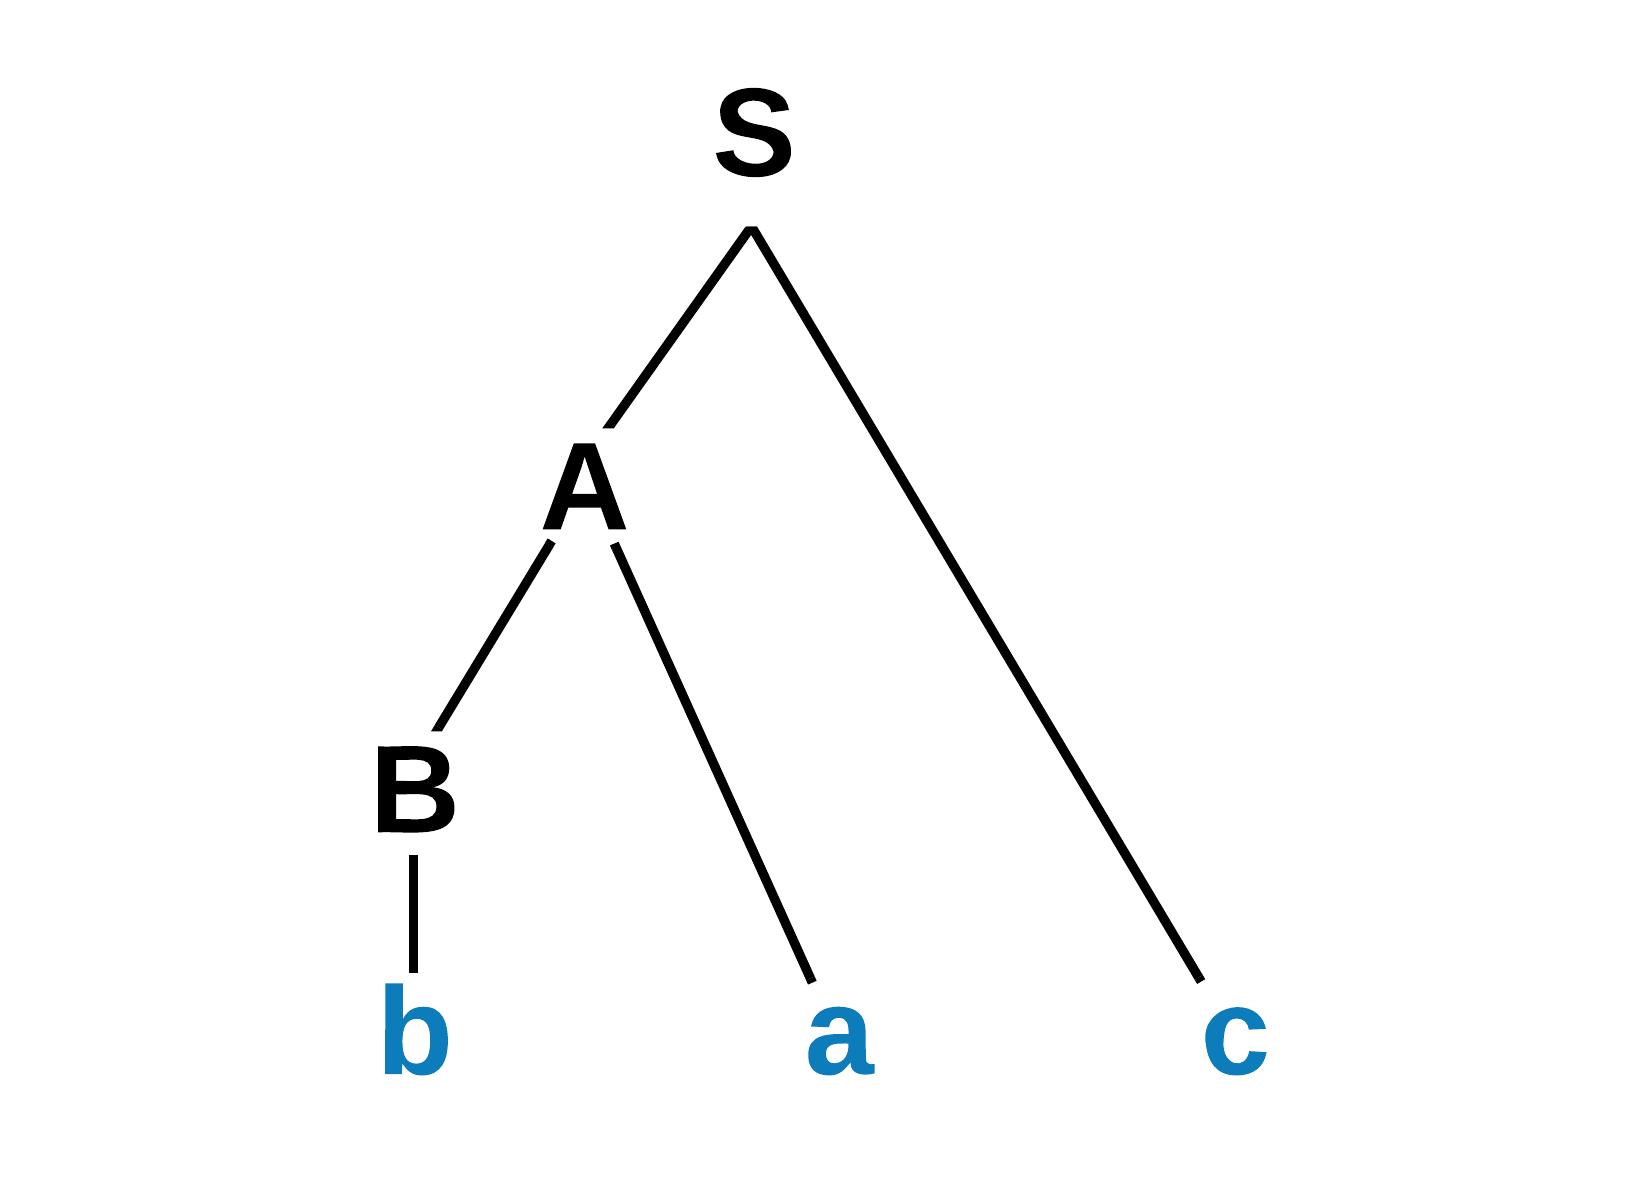
\includegraphics[width=0.5\textwidth]{obrazky-figures/derivationTree.png}
	\caption{Derivačný strom pre bezkontextovú gramatiku $G = (\{S, A, B\}, \{a, b, c\}, \{S\to Ax, A\to Ba, B\to b\}, S)$.}
	\label{derivationTree}
\end{figure}


\subsection{Chomského normálová forma}
\label{CNF}
Pri syntaktickej analýze popísanej v kapitole \ref{syntax} je veľmi dôležité vedieť formu, v akej sú jednotlivé pravidlá danej gramatiky. Pokiaľ je táto forma pravidiel vhodne obmedzená, umožní nám to použitie efektívnejších a sofistikovanejších algoritmov. Jednou z týchto foriem je práve Chomského normálová forma - \textit{CNF}.

\begin{definition}
\label{BKG}
Bezkontextová gramatika $ G = (N, T, P, S) $ je v \textit{Chomského normálovej forme} ak pre každé pravidlo $A \to x \in P $  platí $ x \in NN $ alebo $ x \in T $.


\end{definition}
\hfill\\
Prakticky to znamená, že na pravej strane pravidla sa môžu vyskytovať dva neterminály, alebo jeden terminál.
CNF sa obvykle spája s bezkontextovými gramatikami. Tento princíp však môžeme aplikovať aj pre pravidlá L-systémov.

Každú bezkontextovú gramatiku je možné transformovať do ekvivalentnej bezkontextovej gramatiky v Chomského normálovej forme \cite{medunaBase}. Preto pri práci s týmito gramatikami môžeme automaticky predpokladať, že sú práve v Chomského normálovej forme.

\subsection{Chomského hierarchia}
Rozlišujeme viacero druhov gramatík. Jednu z nich, bezkontextovú gramatiku (viď \ref{BKG}), sme si už popísali, ďalšie si len spomenieme. Tieto gramatiky je možné zoradiť podľa ich vyjadrovacej sily. Čím je gramatika silnejšia, tým viac unikátnych jazykov je pomocou nej možné popísať. Chomského hierarchia rozdeľuje gramatiky podľa ich vyjadrovacej sily do~štyroch rôznych úrovní nazývaných \textit{typ} spolu s číselným označením 0 až 3. Čím je číslo typu nižšie, tým silnejšia je daná gramatika.

\begin{definition}
\label{chomskyGrammars}
Gramatika $G = (N, T, P, S)$ sa označuje ako:

\begin{itemize}
    \itemsep0.2em 
    \item[] \textbf{kontextovo závislá} (anglicky \textit{context-sensitive}), ak pre každé prepisovacie pravidlo $u \to v \in P$ platí, že $u = u_1Au_2, v = u_1xu_2$ pre $u_1, u_2 \in (N \cup T)^*, A \in N, x \in (N \cup T)^+$ a taktiež sa označuje ako \textbf{CS}
    \item[] \textbf{bezkontextová}, ak pre každé prepisovacie pravidlo $u \to v \in P$ platí, že $u \in N$ a taktiež sa označuje ako \textbf{CF}
    \item[] \textbf{lineárna}, ak pre každé prepisovacie pravidlo $u \to v \in P$ platí, že $u \in N$ a $v \in T^* \cup (T^*NT^*)$ a taktiež sa označuje ako \textbf{LIN}
    \item[] \textbf{regulárna}, ak pre každé prepisovacie pravidlo $u \to v \in P$ platí, že $u \in N$ a $v \in T \cup TN \cup \{\epsilon\}$ a taktiež sa označuje ako \textbf{REG}
\end{itemize}

\end{definition}
\hfill\\

Frázové, kontextovo závislé, bezkontextové a regulárne gramatiky sa v Chomského hierarchii označujú ako gramatiky typu 0, typu 1, typu 2, typu 3 v tomto poradí \cite{handbook}.

\begin{definition}[Chomského hierarchia]
Platí nasledovná striktná inklúzia: \[L(REG) \subset L(LIN) \subset L(CF) \subset L(CS) \subset L(RE)\]

\end{definition}

$L()$ predstavuje rodinu jazykov generovanú jednou z gramatík, definovaných v definícii \ref{chomskyGrammars} a $L(RE)$ predstavuje rodinu \textit{rekurzívne vyčísliteľných} jazykov ktoré sú generované frázovými gramatikami.

Táto hierarchia je graficky reprezentovaná na obrázku \ref{chomskyGrammars}.

\begin{figure}[hbt]
	\centering
	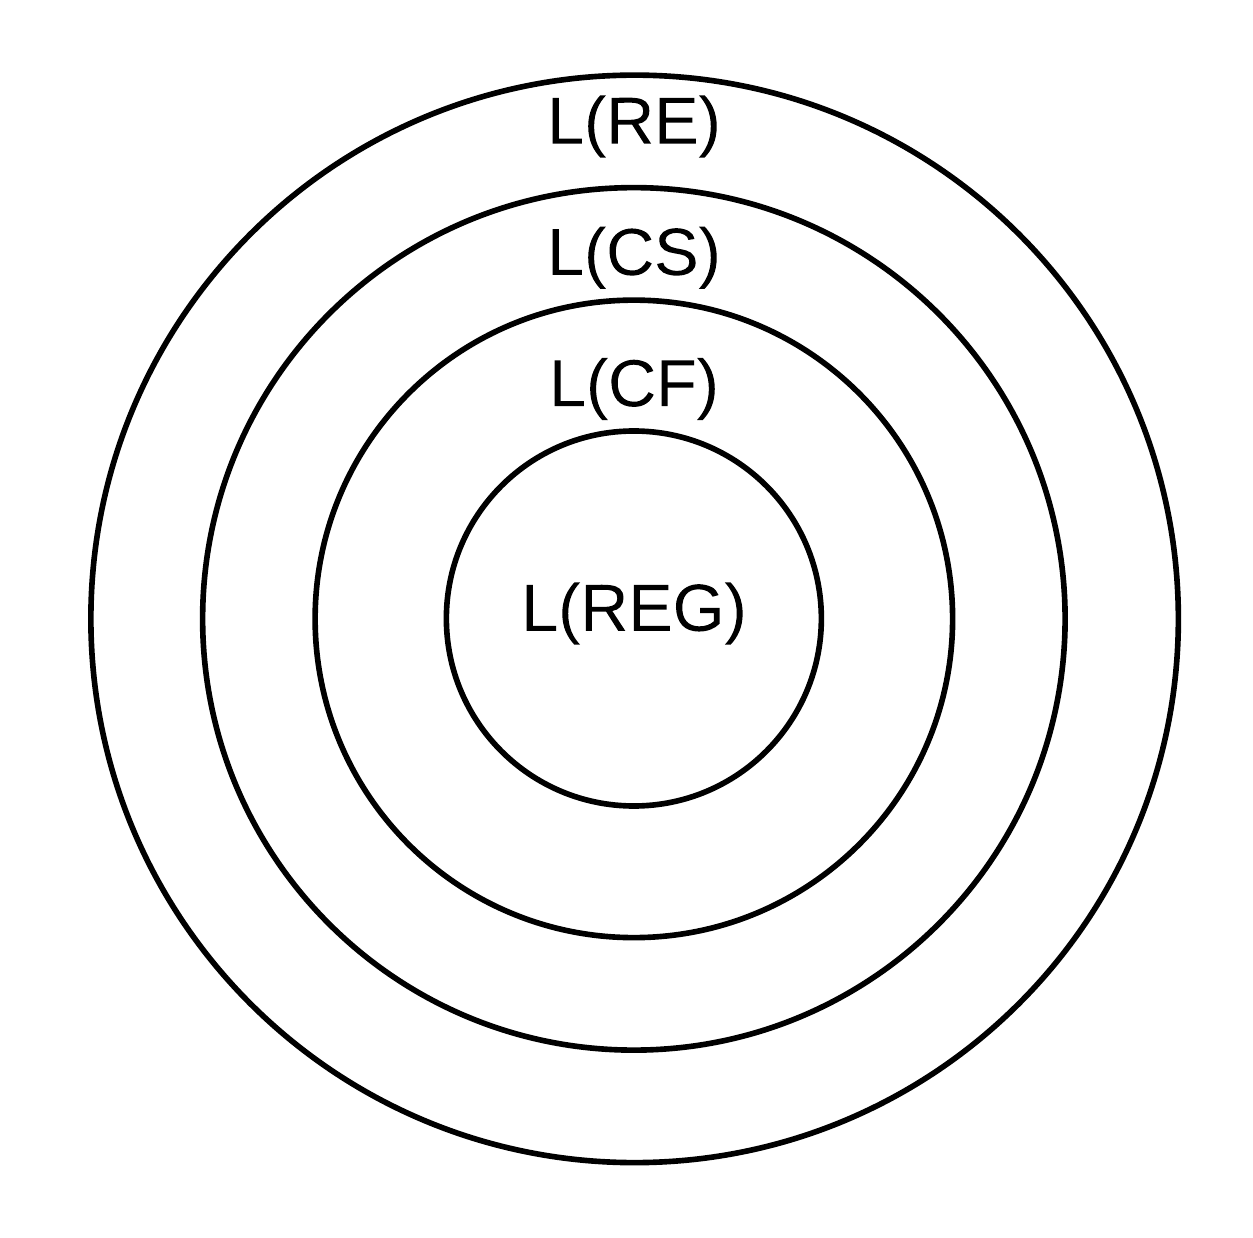
\includegraphics[width=0.5\textwidth]{obrazky-figures/chomskyHierarchy.png}
	\caption{Chomského hierarchia jazykov, kde L(RE), L(CS), L(CF), L(REG) značia rodinu rekurzívne vyčísliteľných, kontextovo závislých, bezkontextových a regulárnych jazykov v~tomto poradí.}
	\label{chomskyHierarchy}
\end{figure}

%=============================================================================================
\chapter{L-systémy}
\label{lsystem}

Lindenmayerove systémy, alebo skrátene L-systémy sú pomenované po biológovi Aristidovi Lindenmayerovi. Ten s ich konceptom prišiel v roku 1968. Boli vytvorené za účelom matematického popisu rastu rastlín a rôznych bunkových organizmov\cite{algBeauty}. Základ L-systémov vznikol samostatne, mimo teoretickú informatiku a až neskôr sa stal súčasťou teoretickej informatiky. Preto sa môžu vyskytovať rôzne inkonzistencie v názvosloví.

V praxi sú L-systémy dobre využiteľné. Umožňujú procedurálne generovať fraktály, rastliny, stromy a pod. Ďalšou výhodou je, že je možné generovať náhodné variácie spomínaných objektov. Preto je ich hlavné využitie v počítačovej grafike. Najčastejším použitím je teda generovanie reťazcov z L-systémov. V tejto práci sa venujeme opačnému problému. A to zisťovaniu, či boli reťazce vygenerované daným L-systémom.

Hlavnou a najpodstatnejšou vlastnosťou L-systémov, ktorou sa odlišujú od ostatných formálnych modelov, je ich \textbf{úplný paralelizmus}. To znamená, že v rámci každého derivačného kroku sa prepisujú všetky symboly slova.

V tejto práci sa zaujímame hlavne o ET0L systémy. Tento názov je zložený z viacerých vlastností L-systémov, ktoré si popíšeme v tejto kapitole.

\section{0L systémy}

Najjednoduchšou formou L-systémov sú práve 0L systémy. Jedná sa o bezkontextové L-systémy, čo značí \textbf{0} v názve (číta sa ako písmeno \uv{o}). Vo svojej podstate sú špeciálnou variantou obyčajných prepisovacích systémov \cite{salomaa} (viď \ref{rewrite}), ktoré ale ako už bolo spomenuté, v rámci svojho derivačného kroku aplikujú všetky možné pravidlá zároveň. Sú teda prepísané všetky znaky v pôvodnom slove.

Tak isto ako prepisovacie systémy, obsahujú len jednu abecedu, ktorá obsahuje len neterminály. Nerozlišujú sa teda terminály a neterminály, ako napríklad v gramatikách (viď \ref{grammar}). To znamená, že po každom derivačnom kroku získavame platný reťazec, ktorý patrí do generovaného jazyka.


\begin{definition}
\label{0L}

0L systém je trojica
\[ G = (\Sigma, P, w_o) \]
kde

\begin{itemize}
    \itemsep0.2em 
    \item[] $ \Sigma $ je abeceda;
    \item[] $ P $ je konečná množina \textit{produkcií} (pravidiel) v tvare $ (a, \alpha) \in P $ označované ako $ a \to \alpha $  \\ kde $ a \in \Sigma $ a $ \alpha \in \Sigma^* $;
    \item[] $ w_o $ je počiatočné slovo nad $ \Sigma$, $w_o \in \Sigma^+ $;
\end{itemize}
\end{definition}
\hfill\\


Produkcie (ďalej pravidlá) sa niekedy v literatúre označujú aj ako \textit{substitúcie}.
Počiatočné slovo $ w_o $ sa často označuje ako \textit{axiom}.


\begin{definition}
Pre 0L systém $G = (\Sigma, P, w_o)$ je \textbf{derivačný krok} $\Rightarrow$ definovaný nasledovne:
\[x_1...x_n \Rightarrow y_1...y_n, \quad\quad n\geq1 \text{ pre každé } x_i \in \Sigma \]

platí, že $x_i \to y_i \in P$ pre každé $i = 1,...,n$. Jazyk generovaný 0L systémom G je definovaný ako $L(G) = \{u | w \Rightarrow^*u\}$.

\end{definition}
\hfill\\

\subsection*{Vlastnosti uzavretí}
Keďže 0L systémy neobsahujú žiadnu formu filtrovania výsledných reťazcov, znamená to, že 0L systémy majú slabé vlastnosti uzavretí. Ináč povedané, nie sú uzavreté nad väčšinou jazykových operácií (viď \ref{closureProperties}).

0L systémy nie sú uzavreté nad týmito operáciami: \textit{zjednotenie, Kleene +, morfizmus, inverzný morfizmus, prienik s regulárnym jazykom, zreťazenie, doplnok} \cite{TIDPresentation}. Niektoré tieto operácie sú definované v časti \ref{closureProperties} a ostatné sú bežné množinové operácie. Porovnanie vlastností uzavretí s inými 0L rodinami je možné vidieť v tabuľke \ref{closurePropertiesTable}.

Rodina jazykov generovaná E0L systémami sa na základe svojich vlastností uzavretí klasifikuje ako \textit{anti-AFL}. Toto označenie je definované v definícii \ref{AFLDefinition}.

\subsection*{Porovnanie s Chomského hierarchiou}
Vďaka úplnému paralelizmu a slabým vlastnostiam uzavretí majú 0L systémy špecifický vzťah ku formálnym gramatikám, pokiaľ porovnávame ich vyjadrovaciu silu.

Rodina jazykov generovaná 0L systémom má prienik s niektorými rodinami v~Chomského hierarchii, konkrétne s rodinami bezkontextových a regulárnych jazykov. Je však podmnožinou kontextovo závislých jazykov. To znamená, že bezkontextové a regulárne rodiny jazykov obsahujú také jazyky, ktoré neobsahuje rodina jazykov 0L. A naopak, 0L rodina jazykov obsahuje jazyky, ktoré neobsahujú rodiny bezkontextových a regulárnych jazykov. Túto hierarchiu aj s príkladmi jazykov je možné vidieť na obrázku \ref{0LHierarchy}.

\begin{figure}[hbt]
	\centering
	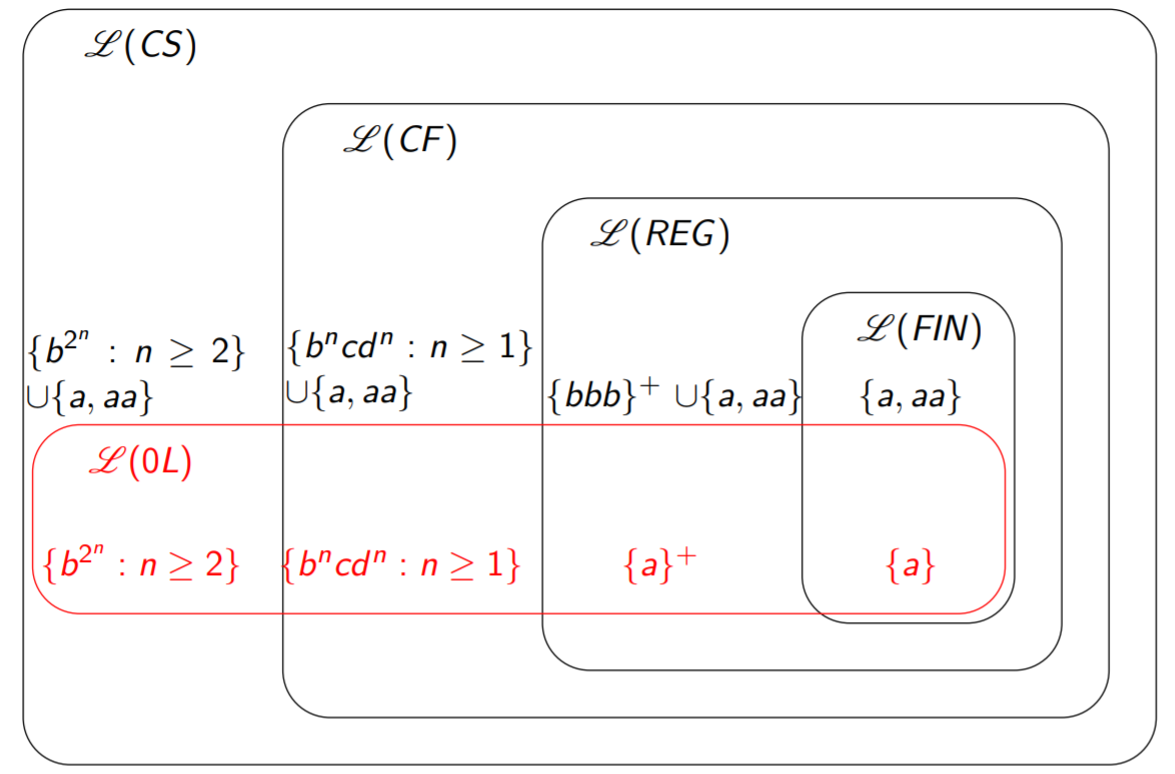
\includegraphics[width=0.8\textwidth]{obrazky-figures/0Lhierarchy.png}
	\caption{0L systémy v kontexte Chomského hierarchia jazykov, kde L(CS), L(CF), L(REG), L(FIN) značia rodinu kontextovo závislých, bezkontextových, regulárnych a konečných jazykov v tomto poradí. Ďalej sú uvedené príklady jazykov ktoré nepatria do rodiny jazykov 0L. Obrázok je prebraný z prezentácie \cite{TIDPresentation}.}
	\label{0LHierarchy}
\end{figure}

\section{Rodiny}
\label{0LFamilies}
0L systémy vo svojej základnej podobe neobsahujú žiadne filtrovacie mechanizmy, musíme teda prijať všetky reťazce vygenerované týmito systémami \cite{handbook}. Táto vlastnosť je však veľmi obmedzujúca, je teda potrebné tento problém vyriešiť. Riešením je zavedenie rôznych filtrovacích mechanizmov. Príkladom takéhoto filtrovania je používanie neterminálov. Tento spôsob používajú napríklad gramatiky (viď \ref{grammar}), ktoré neprijmú reťazec, pokiaľ sa v ňom vyskytuje aspoň jeden neterminál. Ich jazyk teda obsahuje iba také slová, kde je každý ich symbol neterminál.

Takéto filtrovanie do 0L systémov zavádzame pomocou \textit{rodín}. Tieto rodiny rôzne modifikujú 0L systémy, buď rozšíreniami, alebo naopak obmedzeniami. To znamená, že filtrácia je len jedným z dôvodov, prečo sa tieto rodiny používajú.

Rodiny 0L systémov sa označujú pomocou písmena pred označením 0L. Tie sa navyše môžu rôzne kombinovať. Takže rodina ET0L, ktorou sa zaoberáme, znamená kombináciu rodín E a T 0L systémov. To však neznamená, že tieto rodiny sa používajú len pre 0L systémy. Používajú sa aj pre kontextovo závislé L-systémy, kde sa taktiež uvádzajú na~začiatku označenia.

\subsection*{D - deterministic}
Základnou rodinou, ktorá sa v literatúre uvádza sú D0L systémy. Pre rodinu D platí, že množina pravidiel $ P $ obsahuje pre každé $ a \in \Sigma $ práve jedno pravidlo.

Algoritmus pre syntaktickú analýzu (viď \ref{CYK}), ktorý modifikujeme v rámci tejto práce, však zvláda aj nedeterministické gramatiky. Preto sa pri jeho modifikácii pre L-systémy nemusíme obmedzovať determinizmom a tak túto rodinu nepoužívame.

\subsection*{P - propagating}
Táto rodina 0L systémov odstraňuje prázdne prepisovacie pravidlá. Teda pravidlá v tvare $\alpha \to \epsilon$.

V tejto práci sa touto rodinou priamo nezaoberáme, používa sa však v inom existujúcom riešení.

\subsection*{E - extended}
\label{extended}
Pri definícii 0L systému bolo spomenuté, že neobsahujú neterminály. Táto rodina rozširuje 0L systémy práve o neterminály a tým nám umožňuje filtrovať výsledné reťazce. E0L systémy tak majú vyššiu vyjadrovaciu silu než klasické 0L systémy.

Filtrovanie na základe neterminálov funguje tak, že generovaný jazyk nemôže obsahovať reťazce, ktoré obsahujú aspoň jeden neterminál.

Zavedením rodiny E0L získavame systémy veľmi podobné bezkontextovým gramatikám. Rozdiel je v už spomínanej paralelnej aplikácii pravidiel.


\subsection*{T - tables}
\label{tables}
Najvýraznejšou modifikáciou 0L systémov oproti formálnym gramatikám (viď \ref{grammar}) je práve rodina T. Tá zavádza množinu tabuliek pravidiel. Pri každom derivačnom kroku je možné zvoliť tabuľku, z ktorej sa budú pravidlá aplikovať. Tabuľka nie je nič iné, než konečná množina produkcií $P$.

Motivácia zavedenia viacerých tabuliek pravidiel pochádza z premenlivých podmienok pre vývoj rastlín a organizmov. Tými môžu byť rôzne časti dňa, roka alebo odlišné fázy rastu \cite{handbook}.

Táto vlastnosť má zmysel len pri paralelnom prepisovaní. Nakoľko pri sekvenčnom prepisovaní aplikujeme pravidlá jednotlivo, nemá zmysel voliť medzi rôznymi tabuľkami \cite{handbook}.


\hfill\\
Existuje mnoho ďalších rodín 0L systémov. Niektoré z nich zavádzajú spôsoby filtrovania reťazcov, pri ktorých je možné skúmať a porovnávať ich vyjadrovaciu silu. Nimi sa v tejto práci zaoberať nebudeme. 


\section{E0L systémy}
V predchádzajúcej časti \ref{0LFamilies} bola definovaná rodina E 0L systémov ako rozšírenie o~neterminály. E0L systém je teda taký 0L systém, kde je abeceda $\Sigma$ rozdelená na dve disjunktné časti, pričom jedna časť obsahuje terminály a druhá časť obsahuje neterminály. Ako už bolo spomenuté, jazyk generovaný E0L systémom obsahuje len také slová, ktoré neobsahujú neterminály.

Pri popisovaní rodín 0L systémov bolo spomenuté, že tieto rodiny je možné kombinovať a dopracovať sa tak až k ET0L systémom. Preto je definovaný aj E0L systém ako medzikrok, aby sa bolo možné sa prepracovať až k ET0L systémom, ktoré sú hlavným predmetom tejto práce.


\begin{definition}
\label{E0LDefinition}

E0L systém je štvorica

\[ E = (\Sigma, T, P, w_o) \]

kde 

\begin{itemize}
    \itemsep0.2em 
    \item[] $\Sigma$ je celková abeceda
    \item[] $T$ je abeceda terminálov, $ T \subseteq \Sigma $
    \item[] $ P $ je konečná množina \textit{produkcií} (pravidiel) v tvare $ (a, \alpha) \in P $ označované ako $ a \to \alpha $  \\ kde $ a \in \Sigma $ a $ \alpha \in \Sigma^* $;
    \item[] $ w_o $ je počiatočné slovo nad $ \Sigma$, $w_o \in \Sigma^+ $;
\end{itemize}
\end{definition}
\hfill\\

Keďže E0L systémy zavádzajú pomocou abecedy terminálov spôsob filtrovania výsledných slov, zvyšuje sa tým ich vyjadrovacia sila oproti 0L systémom. Rodina jazykov generovaná E0L systémami má taktiež lepšie vlastnosti uzavretí ako 0L systémy. To~znamená, že je uzavretá nad viacerými jazykovými operáciami.

\subsection*{Vlastnosti uzavretí}
Ako bolo spomenuté, modifikáciou E nad 0L systémami sa zlepšujú vlastnosti uzavretí rodiny jazykov E0L systémov. Stáva sa takmer \textit{plne AFL}, je však neuzavretá nad \textit{inverzným morfizmom}.

\subsection*{Porovnanie s bezkontextovou gramatikou}
Pri 0L systémoch bolo spomenuté, že rodina 0L jazykov má prienik s rodinou bezkontextových jazykov. Teda obe obsahujú jazyky, ktoré neobsahuje druhá rodina, neplatí medzi nimi inklúzia. E0L systémy však majú vyššiu vyjadrovaciu silu než 0L systémy a~platí inklúzia $L(CF) \subset L(E0L) \subset L(CS)$, kde $L(CF)$ značí bezkontextovú rodinu jazykov generovanú bezkontextovými gramatikami.

\begin{definition}
\label{BKGtoE0L}
Pre každú bezkontextovú gramatiku $G = (N, T, P, S)$ platí, že ak pre každý symbol $\alpha \in N \cup T$ pridáme prepisovacie pravidlo $\alpha \to \alpha$ a výsledok budeme vnímať ako E0L systém $G_1$, platí jazyková ekvivalencia $L(G) = L(G_1)$.
\end{definition}
\hfill\\
Táto definícia poukazuje na vlastnosť, že každú bezkontextovú gramatiku je možné vyjadriť ekvivalentným E0L systémom\cite{salomaa}.

\section{ET0L systémy}
Najviac študovanou rodinou L-systémov sú práve ET0L systémy vďaka svojím vhodným matematickým vlastnostiam a silným vlastnostiam uzavretí nad operáciami (anglicky \textit{closure properties}).
Ako bolo spomenuté, jednotlivé rodiny je možné kombinovať, takže ET0L systém je rozšírením 0L systému o abecedu neterminálov a množiny tabuliek pravidiel. Je to kombinácia rodín E (extended) a T (tables).

\begin{definition}
\label{ET0LDefinition}
ET0L systém je (n + 3)-tica

\[ E = (\Sigma, T, P_1, P_2, ..., P_n, w_o) \]

kde 

\begin{itemize}
    \itemsep0.2em 
    \item[] $n \geq 1$
    \item[] pre všetky $ i = 1, ..., n$, $E_i = (V, T, P_i, w)$ je E0L systém
\end{itemize}
\end{definition}
\hfill\\

Predpokladáme, že každá tabuľka obsahuje pre každé $ a \in \Sigma $ aspoň jedno pravidlo.

\subsection*{Počet tabuliek}
ET0L systémy nijako neobmedzujú počet tabuliek, ktoré obsahujú. Môžu teda teoreticky obsahovať nekonečno týchto tabuliek. Vyplýva teda otázka, ako sa menia vlastnosti ET0L systémov v závislosti na počte týchto tabuliek.

Na počte tabuliek v ET0L systémoch nezáleží. Platí totiž, že pre každý ET0L systém existuje ekvivalentný ET0L systém s \textbf{dvoma tabuľkami}\cite{handbook}.

\subsection*{Derivačný krok}
Pri každej aplikácii pravidiel, teda pri \textbf{derivačnom kroku}, je nutné vybrať si jednu z~tabuliek pravidiel, z ktorej sa budú tieto pravidlá používať. Neexistuje žiadne pravidlo, ktoré by hovorilo, ktorá tabuľka má byť, alebo naopak, nemôže byť použitá. Môže byť teda vybratá ľubovoľná tabuľka $P_i$. V rámci daného derivačného kroku sa však môžu aplikovať pravidlá iba z jednej tabuľky.

\begin{definition}
Pre ET0L systém $G = (\Sigma, T, P_1, ..., P_n, w_o)$  je \textbf{derivačný krok} $\Rightarrow$ definovaný nasledovne:
\[x_1...x_n \Rightarrow y_1...y_n, \quad\quad n\geq1 \text{ pre každé } x_i \in \Sigma \]

platí, že $x_i \to y_i \in G_k = (\Sigma, T, P_k, w_o)$ pre každé $i = 1,...,n$. Pričom $G_k$ je E0L systém podľa definície \ref{ET0LDefinition}.
\end{definition}

\subsection*{Vlastnosti uzavretí}
Zavedením rodiny T k už existujúcim E0L systémom sa zlepšujú aj vlastnosti uzavretí týchto L-systémov. Konkrétne, ET0L systémy sa označujú ako \textit{plne AFL}, čo znamená, že oproti E0L systémom sú navyše uzavreté nad operáciou inverzného morfizmu. Pokiaľ uvažujeme rodinu T0L, teda bez rodiny E, tak ide o \textit{anti AFL} rodinu, rovnako ako je to pri 0L systémoch\cite{handbook}.

\subsection*{Porovnanie s Chomského hierarchiou}
Rozšírenie E0L systémov o rodinu T zvyšuje vyjadrovaciu silu výsledných ET0L systémov podobne, ako sa zlepšili ich vlastnosti uzavretí. Stávajú sa tak nadmnožinou E0L systémov, ale stále majú nižšiu vyjadrovaciu silu, než rodina kontextovo závislých jazykov a sú ich podmnožinou. Platí teda vzťah:
\[L(CF) \subset L(E0L) \subset L(ET0L) \subset L(CS)\]
Porovnanie vlastností uzavretí gramatík z Chomského hierarchie a L-systémov definovaných v tejto kapitole je možné vidieť v tabuľke \ref{closurePropertiesTable}.

\begin{table}[]
    \centering
    \begin{tabular}{|c||c|c|c|c||c|c|c|}
    \hline
        & RE & CS & CF & REG & 0L & E0L & ET0L\\
    \hline
        Zjednotenie & $\checkmark$ & $\checkmark$ & $\checkmark$ & $\checkmark$ 
        & $\times$ & $\checkmark$ & $\checkmark$ \\
    \hline
        Prienik & $\checkmark$ & $\checkmark$ & $\times$ & $\checkmark$
        &  &  &  \\
    \hline
        Doplnok & $\times$ & $\checkmark$ & $\times$ & $\checkmark$
        & $\checkmark$ & $\checkmark$ & $\checkmark$ \\
    \hline
        Zreťazenie & $\checkmark$ & $\checkmark$ & $\checkmark$ & $\checkmark$
        & $\times$ & $\checkmark$ & $\checkmark$ \\
    \hline
        Kleene star (*) & $\checkmark$ & $\checkmark$ & $\checkmark$ & $\checkmark$
        & $\times$ & $\checkmark$ & $\checkmark$ \\
    \hline
        Substitúcia & $\checkmark$ & $\times$ & $\checkmark$ & $\checkmark$
        &  &  &  \\
    \hline
        Morfizmus & $\checkmark$ & $\times$ & $\checkmark$ & $\checkmark$
        & $\times$ & $\checkmark$ & $\checkmark$ \\
    \hline
        Inverzný morfizmus & $\checkmark$ & $\checkmark$ & $\checkmark$ & $\checkmark$
        & $\times$ & $\times$ & $\checkmark$ \\
    \hline
    \end{tabular}
    \caption{Vlastnosti uzavretí rodín jazykov z Chomského hierarchie a rodín jazykov L systémov. Prevzaté z knihy \cite{handbook} a prezentácie \cite{TIDPresentation}.}
    \label{closurePropertiesTable}
\end{table}

\section{Chomského normálová forma E0L a ET0L systémov}
\label{chomskyDegradation}
Pri bezkontextových gramatikách bola definovaná aj ich Chomského normálová forma \ref{CNF}. V skratke sa jedná o tvar pravidiel, do ktorého je možné transformovať ľubovoľnú bezkontextovú gramatiku, pričom výsledná gramatika jej bude ekvivalentná. Táto forma sa využíva pri algoritme Cocke-Younger-Kasami (viď \ref{CYK}). Preto je v rámci tejto práce Chomského normálová forma žiadaná aj pre E0L a ET0L systémy. Umožňuje totiž pomocou istých modifikácií využiť spomínaný algoritmus CYK aj pre tieto systémy.

0L systémy všeobecne obsahujú prepisovacie pravidlá pre terminály (0L systémy nerozoznávajú terminály a neterminály, všetky symboly sa môžu považovať za terminály). Pri bezkontextových gramatikách takéto pravidlá neexistujú, prepisujú sa teda len neterminály. Chomského normálová forma teda s takýmito pravidlami nepočíta. Preto v~prípade E0L a ET0L systémov musíme uvažovať implicitné pravidlo $\alpha \to \alpha$, ináč povedané, terminály sa neprepisujú. Ignorujú sa. Ďalej sa obmedzí axiom na počiatočný symbol z~abecedy neterminálov.

\subsection*{Degradácia vyjadrovacej sily použitím Chomského normálovej formy}


Zavedenie tejto normálovej formy však spôsobuje vážny problém pre E0L a následne aj pre ET0L systémy. Ten vyplýva z definície \ref{BKGtoE0L}. Pokiaľ zapíšeme pravidlá v Chomského normálovej forme a pre terminály uvažujeme spomínané implicitné pravidlo $\alpha \to \alpha$, získavame tak E0L systém, ktorý je ekvivalentný bezkontextovej gramatike s rovnakými pravidlami. Znamená to, že pri použití tejto normálovej formy degradujeme vyjadrovaciu silu E0L systémov na tú bezkontextových gramatík. To ovplyvní aj ET0L systémy.

\section{Normálová forma E0L a ET0L systémov}
\label{E0LNormalForm}
Existuje normálová forma, pomocou ktorej je možné pre každý E0L systém vyjadriť ekvivalentný E0L systém. Táto normálová forma obsahuje pravidlá v nasledovnom tvare:

\[
    A \to a, \quad\quad A \to B, \quad\quad A \to BC, \quad\quad a \to A, \quad\quad A \to \epsilon; \quad \quad
\]

kde $A$, $B$, $C$ sú ľubovoľné neterminály a $a$ je ľubovoľný terminál. Táto normálová forma je prevzatá z knihy \cite{mathTheoryL}.

V definícii ET0L systémov \ref{ET0LDefinition} je ET0L systém definovaný pomocou E0L systémov. Pre každú tabuľku, ktorú obsahuje, existuje E0L systém. Preto pokiaľ transformujeme každú tabuľku do tejto normálovej formy, získame ekvivalentný ET0L systém.

Oproti Chomského normálovej forme sa táto normálová forma líši prepisovaním jedného terminálu na neterminál alebo naopak. Taktiež sú povolené takzvané prázdne prepisovacie pravidlá, teda prepisovaný neterminál sa vymaže. To je značené symbolom $\epsilon$.



\section{Kontextová závislosť}
V rámci tejto kapitoly sa rozoberali len bezkontextové L-systémy, v ktorých sa táto bezkontextovosť označuje pomocou \uv{0} v názve. Za zmienku však stoja aj kontextovo závislé L-systémy, ktoré sa označujú ako \textbf{interaktívne L-systémy} a skratkou \textbf{IL systémy} kde \uv{\textit{I}} znamená interaktívnosť. 

Kontextovosť sa označuje ako $(m, n)L$ systém, kde $m, n \geq 0$ a má pravidlá v tvare\cite{handbook}
\[ (\alpha, a, \beta) \to w \quad\text{kde}\quad |\alpha|=m, |\beta|=n \]

Z tohto tvaru pravidiel je zjavné, že prvé číslo $m$ v zátvorke značí počet symbolov, ktoré sú vnímané ako súčasť kontextu na ľavej strane prepisovaného symbolu a druhé číslo $n$ značí zasa pravú stranu.

Kontextová závislosť pri bezkontextových L-systémoch by sa teda v tejto notácii značila ako (0, 0). Toto značenie sa však skracuje na \textbf{0}.

%=============================================================================================
\chapter{Syntaktická analýza} 
\label{syntax}

S niektorými formami syntaktickej analýzy sa v informatike, hlavne pri programovaní, stretávame pravidelne. Pri prirodzených jazykoch môžeme za istú formu syntaktickej analýzy považovať kontrolu gramatiky a vetnej skladby. Túto kontrolu vykonáva človek, ktorý dokáže zmyslu vety porozumieť aj napriek istému počtu chýb. Na rozdiel od ľudí však počítač potrebuje presnú formu jazyka, ktorému má rozumieť a vyžaduje jeho striktné dodržiavanie.

V informatike sa syntaktická analýza používa v prekladačoch programovacích jazykov a tvorí ich hlavnú časť. Programovacie jazyky majú presne definovanú syntax, preto je možné ju použitím špecifických algoritmov kontrolovať. Nie všetky aspekty programovacích jazykov je možné vyjadriť formálne pomocou nejakej formy zápisu, preto sa v praxi bežne kombinuje syntaktická analýza so sémantickou analýzou. Príkladom môže byť kontrola existencie premenných.

V tejto práci sa venujeme samostatnej syntaktickej analýze. Jej cieľom je zistiť, či prijímaný reťazec patrí do jazyka, ktorý je generovaný daným formálnym modelom (viď \ref{formalModel}), konkrétne L-systémom. Ináč povedané, má za úlohu zistiť, či je možné pomocou konkrétnej gramatiky, prepisovacieho systému, alebo iného modelu, vygenerovať požadovaný reťazec.

\section{Druhy syntaktickej analýzy}
\label{analysysTypes}
Existuje mnoho rôznych algoritmov pre syntaktickú analýzu, ktoré môžeme rozdeliť do~dvoch hlavných skupín. Toto rozdelenie je na základe toho, akým spôsobom sa snažíme k~výsledku dopracovať. Algoritmus môže začať počiatočným symbolom a snažiť sa aplikáciou pravidiel získať výsledne slovo. Druhou možnosťou je presne opačný postup, kedy algoritmus začína celým slovom a snaží sa spätne zistiť, či mohlo byť vygenerované pomocou počiatočného symbolu.



\subsection*{Analýza zhora-dole}
Ako vrch a spodok implikovaný z názvu chápeme vrch a spodok derivačného stromu. Myšlienkou takejto analýzy (anglicky \textit{top-down}) je prepracovať sa aplikáciou prepisovacích pravidiel z počiatočného symbolu až ku kontrolovanému reťazcu. Tieto analýzy bývajú oproti analýzam zdola-hore jednoduchšie. Postupne generujú všetky možnosti a snažia sa nájsť zhodu. Často pri tom využívajú rekurziu.

Príkladom je algoritmus \textit{recursive descent}, ktorý sa využíva pri syntaktickej analýze programovacích jazykov.

Vizuálnu reprezentáciu tohto spôsobu je možné vidieť na obrázku \ref{topDownPicture}.

\begin{figure}[hbt]
	\centering
	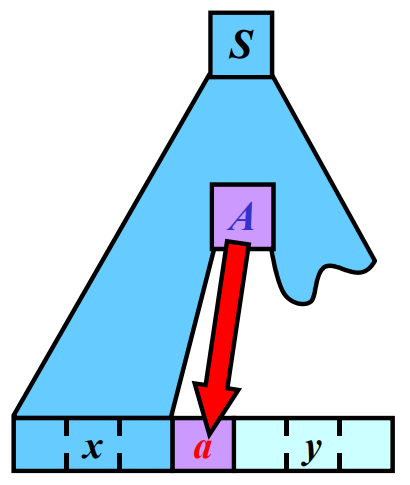
\includegraphics[width=0.3\textwidth]{obrazky-figures/topDown.png}
	\caption{Vizuálna reprezentácia princípu syntaktickej analýzy zhora-dole. Obrázok je prevzatý z prezentácie \cite{IFJPresentation}.}
	\label{topDownPicture}
\end{figure}

\subsection*{Analýza zdola-hore}
Tento spôsob syntaktickej analýzy sa v angličtine označuje ako \textit{bottom-up parsing}. Spodok z~názvu implikovaného derivačného stromu predstavuje reťazec, ktorý kontrolujeme. Znamená to, že sa snažíme spätne prepracovať z reťazca naspäť na vrch derivačného stromu. Ináč povedané ku počiatočnému symbolu. Tieto algoritmy bývajú efektívnejšie, nakoľko nemusia prechádzať všetky variácie derivačného stromu.

Príkladom takéhoto algoritmu je precedenčná analýza používaná na preklad výrazov.
\hfill\\

Oba spomenuté spôsoby syntaktickej analýzy sú bežne používané. Nie je možné povedať, ktorý z nich je lepší, nakoľko oba sú vhodné na iné druhy problémov. Preto sa napríklad v~rámci jedného prekladača bežne vyskytujú oba tieto spôsoby syntaktickej analýzy.

\section{Algoritmus Cocke-Younger-Kasami}
\label{CYK}
Jedná sa o algoritmus zo skupiny syntaktických analýz zdola-hore. To znamená, že postupnými redukciami výsledného slova pomocou prepisovacích pravidiel sa snaží prepracovať až k~počiatočnému znaku. Tento algoritmus bol zvolený ako základ pre~syntaktickú analýzu ET0L systémov. Neskôr je v rámci tejto kapitoly popísané, aké zmeny je potrebné vykonať, aby tento algoritmus dokázal spracovávať aj ET0L systémy.

Algoritmus Cocke-Younger-Kasami (ďalej len CYK) vykonáva syntaktickú analýzu bezkontextových gramatík. Podmienkou, aby mohol byť algoritmus CYK vykonaný je, aby bola vstupná gramatika v Chomského normálovej forme (viď \ref{CNF}). To v skratke znamená, že na pravej strane prepisovacích pravidiel môžu byť len dva neterminály alebo jeden terminál.

Vďaka tomu, že vstupná gramatika musí byť v Chomského normálovej forme, môže byť táto vlastnosť vhodne využitá algoritmom CYK. V tabuľke, s ktorou algoritmus CYK pracuje, sa vyhľadávajú práve dvojice vyplývajúce z Chomského normálovej formy.

Dôležitou vlastnosťou algoritmu CYK je, že zvláda nedeterministické gramatiky. Vstupná gramatika teda môže obsahovať viac pravidiel pre jeden neterminál.


\subsection*{Popis fungovania}

Pri vysvetlení algoritmu sú použité symboly bezkontextových gramatík z definície \ref{BKG} a~predpokladáme bezkontextovú gramatiku $G = (N, T, P, S)$, ktorá slúži ako vstupná gramatika.
Ako bolo spomenuté, algoritmus CYK pracuje na báze zdola-hore, teda analýza začína vstupným slovom $w$ a snaží sa dopracovať až k počiatočnému symbolu $S$.

Zavádza sa tabuľka $CYK[i, j]$, kde $1 \leq i \leq j \leq n$, pričom $n$ je dĺžka vstupného slova $w$. Táto tabuľka sa počas vykonávania algoritmu využíva na vyhľadávanie dvojíc pravých strán pravidiel. Pri nájdení takej dvojice nastáva redukcia pravidla na jeho ľavú stranu (podľa Chomského normálovej formy jeden neterminál) a daný neterminál sa zapíše do tabuľky.

Na úplnom začiatku je nutné do tabuľky $CYK$ vložiť vstupné slovo $w$. To funguje tak, že na diagonálu tabuľky $CYK$ sa umiestnia neterminály, pomocou ktorých je možné priamo derivovať (viď \ref{derivation}) neterminál na rovnakej pozícii vo vstupnom slove $w$. Využité je pravidlo z Chomského normálovej formy, kde je na pravej strane jeden terminál. Pre každé $A \in CYK[i, i]$ platí, že $A \to w_i \in P$ pričom $w_i$ je i-ty znak vo vstupnom slove $w$.

Potom sa v tabuľke CYK vyhľadávajú také dvojice neterminálov, kde platí $B \in CYK[i, j], C \in CYK[j+1, k]$ a $A \to BC \in P$, potom zapíšeme A do CYK[i, k]. Keďže sú bezkontextové gramatiky sekvenčné, každý zapísaný neterminál je používaný v nasledovnom hľadaní dvojíc. Toto hľadanie dvojíc sa vykonáva dovtedy, kým je možné nájsť novú, teda unikátnu dvojicu.

Algoritmus je úspešný, pokiaľ sa nachádza počiatočný symbol $S$ v CYK[1, n]. Vysvetlenie algoritmu je parafrázované z knihy \cite{medunaParser}. Popis algoritmu CYK pre bezkontextové gramatiky je ekvivalentne popísaný pomocou pseudokódu \ref{CYKBKG}. Príkladná vizualizácia fungovania tohto algoritmu je viditeľná na obrázku \ref{CYKTable}.

\hfill\\
Každú bezkontextovú gramatiku je možné previesť na ekvivalentnú bezkontextovú gramatiku v Chomského normálovej forme \cite{medunaBase}. To znamená, že tento algoritmus je možné aplikovať na ľubovoľnú bezkontextovú gramatiku, ktorú je však najprv nutné previesť do~Chomského normálovej formy.


\begin{figure}[hbt]
	\centering
	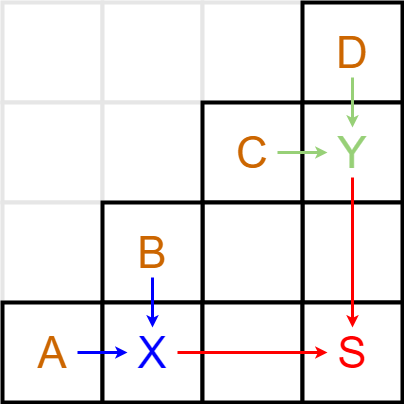
\includegraphics[width=0.3\textwidth]{obrazky-figures/CYKTable.png}
	\caption{Príklad úspešného vykonania algoritmu CYK s vizualizáciou tabuľky CYK pre gramatiku $G = (\{A, B, C, D, X, Y, S\}, \{a, b, c, d\}, \{S \to XY, X \to AB, Y \to CD, A \to a, B \to b, C \to c, D \to d, S\})$ pre~vstupné slovo $abcd$. Spodný ľavý roh predstavuje pozíciu [1, 1] a spodný pravý roh pozíciu [1,4] v tabuľke CYK.}
	\label{CYKTable}
\end{figure}

\begin{algorithm}
\caption{Algoritmus syntaktickej analýzy Cocke-Younger-Kasami pre bezkontextové gramatiky}
\label{CYKBKG}

\textbf{Input}
\setlist{nolistsep}
\begin{itemize}[noitemsep]
    \item grammar, \(G = ({}_G\Sigma, {}_GR)\) in Chomsky normal form
    \item \(w = a_1a_2...a_n\)  where  \(a_i \in {}_G\Delta, 1 \leq i \leq n \), for some \(n \geq 1\).
\end{itemize}
\textbf{Output} 
\begin{itemize}[noitemsep]
    \item \textbf{ACCEPT} if \(w \in L(G)\)
    \item \textbf{REJECT} if \(w\notin L(G)\)
\end{itemize}
\textbf{Method}
\begin{algorithmic}
\State $ CYK[i,j] = \varnothing$ for $1 \leq i \leq j \leq n $
\For{i = i \textbf{to} $n$}
    \If{$ A \rightarrow a_i \in R $}
        \State $add\ A\ to\ CYK[i,i]$
    \EndIf
\EndFor
\Repeat
\If{$ B \in CYK[i,j], C \in CYK[j+1,k], A \rightarrow BC \in R $ for some $A,B,C \in {}_GN$}
\State $add\ A\ to\ CYK[i,k]$
\EndIf
\Until{no changes}
\If{$ S \in CYK[1,n] $}
    \State \textbf{ACCEPT}
\Else
    \State \textbf{REJECT}
\EndIf

\end{algorithmic}
\end{algorithm}

\section{CYK pre rôzne 0L systémy}
Hlavný rozdiel 0L systémov oproti bezkontextovým gramatikám je paralelná aplikácia pravidiel na rozdiel od sekvenčnej aplikácie pravidiel bezkontextových gramatík. To~znamená, že všetky pravidlá musia byť aplikované zároveň. Algoritmus \textit{CYK} je možné vhodnou modifikáciou upraviť tak, aby túto skutočnosť reflektoval.

Dôležitým rozdielom je aj používaná normálová forma. Algoritmus CYK pracuje s~bezkontextovými gramatikami v Chomského normálovej forme. Táto forma pravidiel však nevyhovuje pre použitie s E0L a ET0L systémami, nakoľko obmedzuje ich vyjadrovaciu silu. Preto je používaná normálová forma definovaná v časti \ref{E0LNormalForm}. Rozdiely v tejto normálovej forme oproti Chomského normálovej forme je potrebné zohľadniť pri modifikácii algoritmu CYK. Unárne pravidlá tejto normálovej formy môžeme generalizovať na tvar $\alpha \to \alpha$, pričom $\alpha$ je ľubovoľný znak z celkovej abecedy $\Sigma$.


Ďalším rozdielom, ktorým sa zaoberáme, sú tabuľky (viď \ref{tables}) ET0L systémov. Pre tieto systémy platí, že pred každou aplikáciou pravidiel je zvolená tabuľka pravidiel a pri aplikácii pravidiel sa používajú len pravidlá, ktoré patria do danej tabuľky. Túto vlastnosť je tak isto možné vhodnou modifikáciou algoritmu \textit{CYK} aplikovať.

Podobne ako môžeme kombinovať rôzne rodiny 0L systémov, môžeme kombinovať aj syntaktickú analýzu pre zložené rodiny, napríklad ET0L, a aplikovať v nej modifikácie pre~každú rodinu z ktorej sa skladá. V našom prípade to znamená modifikovať algoritmus \textit{CYK} pre E0L systémy a nad touto modifikáciou aplikovať modifikáciu pre tabuľky T, takže získame modifikáciu pre ET0L systémy.

\subsection*{Množina $empty$ pre prázdne prepisovacie pravidlá}
Normálová forma \ref{E0LNormalForm} pre E0L a ET0L systémy povoľuje takzvané prázdne prepisovacie pravidlá. Chomského normálová forma, ktorá sa využíva v algoritme CYK, však s takýmito pravidlami nepočíta. Preto pre ne nie je tabuľka CYK prispôsobená.

Veľkosť tabuľky CYK je určená spracovávaným slovom. To však pri existencii prázdnych prepisovacích pravidiel môže byť počas derivácie dlhšie než výsledné slovo. Preto nie je možné v tabuľke reprezentovať symboly, ktoré boli počas derivácie zmazané.

Symboly, ktoré môžu byť zmazané nie sú len tie neterminály, ktoré môžu byť priamo zmazané. Zmazanie symbolu môže nastať aj po istej postupnosti aplikácie prepisovacích pravidiel. Ako príklad uvažujme prepisovacie pravidlá \[\{S \to AX, A \to BC, B \to D, C \to \epsilon, D \to \epsilon, X \to x, x \to x\}\] Priamo zmazané môžu byť neterminály $C, D$. Postupnou aplikáciou pravidiel však môžu byť zmazané aj neterminály $A, B$. Pre zredukovanie pravidla $S \to AX$ je potrebné vedieť, že $A$ mohlo byť zmazané a preto sa v tabuľke CYK nenachádza. Neterminál $A$ je však možné vymazať až po istom počte derivačných krokov.

V prípade, že by neexistovalo pravidlo $x \to x$, nebolo by možné vytvoriť žiadne slovo, nakoľko neterminál $A$ by nebo možné zmazať dostatočne rýchlo a $x$ by nemalo žiadne existujúce prepisovacie pravidlo. Ďalším problémom existencie prázdnych pravidiel je, že nie je možné povedať, počas ktorého kroku bol symbol zmazaný. 

Riešením tohto problému je množina $empty$. Tá obsahuje všetky symboly, ktoré môžu byť v aktuálnom kroku zmazané. Túto množinu je potrebné na začiatku každého kroku prepočítať.

Algoritmus výpočtu množiny $empty$ funguje následovne. Vstup algoritmu tvorí stará množina $empty$ nazvaná $emptyOld$ (pri prvom kroku prázdna) a množina prepisovacích pravidiel $P$ v normálovej forme \ref{E0LNormalForm}.

Pre každé pravidlo $A \to B$, $A \to BC$, $A \to \epsilon$ $\in P$, kde $A \in emptyOld$ sa pridá ľavá strana tohto pravidla do množiny $empty$. Takto je zaručené, že množina $empty$ obsahuje len také symboly, ktoré mohli byť v rámci daného kroku skutočne zmazané.


\subsection*{E0L systémy}
\label{EOL parsing}
Pre E0L systémy musíme zaviesť modifikáciu paralelnej aplikácie pravidiel. To docielime tak, že zavedieme novú tabuľku CYKNext, ktorá má totožné vlastnosti ako tabuľka CYK. Do tejto novo zavedenej tabuľky sa budú ukladať novo zredukované neterminály. Algoritmus ďalej rozdelíme na kroky. V rámci kroku sa zredukujú všetky možné pravidlá z tabuľky CYK do novej tabuľky CYKNext. Na konci kroku sa obsah tabuľky CYKNext presunie do tabuľky CYK a tabuľka CYKNext sa vyprázdni. Týmto spôsobom algoritmus dosahuje požadovanú paralelnú aplikáciu pravidiel.

Taktiež sú zohľadnené rozdiely v použitej normálovej forme (viď \ref{E0LNormalForm}) oproti Chomského normálovej forme, ktorá sa používa v pôvodnom CYK algoritme pre bezkontextové gramatiky.


\subsection*{Popis fungovania}
Pri popise sa využíva E0L systém $E = (\Sigma, T, P, w_o)$. Tabuľka CYK a premenné $i, j$ sú rovnaké ako pri CYK pre bezkontextové gramatiky (viď \ref{CYK}). Počiatočné naplnenie tabuľky CYK prebieha rovnako ako v pôvodnom algoritme CYK. 

Prehľadávanie tabuľky CYK pre redukciu pravých strán pravidiel rozdelíme do krokov. Ako redukciu chápeme nájdenie pravej strany pravidla v tabuľke a vloženie ľavej strany pravidla do tabuľky. V rámci kroku hľadáme pravé strany, ktoré je možné zredukovať podobne ako pri pôvodnom algoritme \textit{CYK}.

Rozdiel však nastáva pri vkladaní ľavého neterminálu pravidla do tabuľky pri redukcii. Ten vkladáme do tabuľky CYKNext. Keďže prehľadávame len tabuľku CYK, tak tieto nájdené neterminály nemôžeme v rámci toho istého kroku použiť. Krok končí, keď už nie je možné vykonať novú redukciu.

Využívaná normálová forma umožňuje nasledovné pravé strany pravidiel: dvojicu neterminálov, jeden neterminál, jeden terminál a $\epsilon$. Redukcia páru neterminálov prebieha rovnako ako pri pôvodnom algoritme CYK. Pre každé $A \in CYK[i, j]$, pre ktoré platí $\alpha \to A$, pridáme $\alpha$ do $CYKNext[i, j]$, $\alpha, A \in \Sigma$.

Je prepočítaná množina $empty$ obsahujúca všetky ľavé strany, ktoré môžu byť priamo alebo tranzitívne prepísané na $\epsilon$. Pre každú dvojicu neterminálov, kde platí $B \in CYK[i, j] \land C \in empty$ alebo $B \in empty \land C \in CYK[i, j]$ a existuje $A \to BC \in P$, vložíme A do~$CYKNext[i, j]$.

Na konci každého kroku sa obsah tabuliek $CYK$ a $CYKNext$ vymení a tabuľka $CYKNext$ sa vyprázdni. Získavame tak teda spomínaný paralelizmus. Krok teda chápeme ako jednu paralelnú aplikáciu pravidiel.

Keďže normálová forma \ref{E0LNormalForm} obsahuje unárne pravidlá, teda na pravej strane pravidla je jeden symbol, môže dôjsť k zacykleniu algoritmu. Napríklad, pokiaľ uvažujeme počiatočný symbol $S$, a pravidlá $S \to A, A \to S$. Preto je zavedená množina minulých stavov tabuliek a množín prázdnych stavov $history$. Na konci kroku sa skontroluje, či množina $history$ obsahuje dvojicu aktuálnej tabuľky $CYKNext$ a množiny $empty$ ešte pred výmenou obsahu $CYK$ a $CYKNext$. Pokiaľ áno, je detekovaný cyklus a algoritmus končí neúspechom. Ináč je táto dvojica pridaná do množiny prázdnych stavov $history$.Princíp tejto detekcie je prevzatý z~diplomovej práce \cite{FITMT21128}.

Algoritmus končí úspechom, pokiaľ sa v ľubovoľnom kroku na pozíciu CYKNext[1, n] dostane počiatočný symbol. Ukončenie algoritmu nastáva vtedy, ak tabuľka CYKNext neobsahuje žiaden nový neterminál. Algoritmus je taktiež popísaný pomocou pseudokódu \ref{CYKE0L}.


\begin{algorithm}
\caption{Cocke-Younger-Kasami algoritmus syntaktickej analýzy pre E0L systémy}
\label{CYKE0L}

\textbf{Input}
\setlist{nolistsep}
\begin{itemize}[noitemsep]
    \item E0L system, \(E = (\Sigma, T, P, w_o)\) in normal form \ref{E0LNormalForm}
    \item \(w = a_1a_2...a_n\)  where  \(a_i \in {}_E\Delta, 1 \leq i \leq n \), for some \(n \geq 1\).
\end{itemize}
\textbf{Output} 
\begin{itemize}[noitemsep]
    \item \textbf{ACCEPT} if \(w \in L(G)\)
    \item \textbf{REJECT} if \(w\notin L(G)\)
\end{itemize}
\textbf{Method}
\begin{algorithmic}
\State $ CYK[i,j] = \varnothing$ for $1 \leq i \leq j \leq n $
\State $ CYKNext[i,j] = \varnothing$ for $1 \leq i \leq j \leq n $
\State $ empty\ = \varnothing$
\State $history = \varnothing$
\For{i = i \textbf{to} $n$}
    \If{$ A \rightarrow a_i \in P $}
        \State $add\ A\ to\ CYK[i,i]$
        \State $add\ A\ to\ CYKNext[i,i]$
    \EndIf
\EndFor

\Repeat
\State calculate empty
\If{$ A \in CYK[i,j], \alpha \rightarrow A \in R $ for some $A, \alpha \in \Sigma$}
\State $add\ \alpha\ to\ CYKNext[i,j]$
\EndIf

\If{$ B \in CYK[i,j], C \in empty, A \rightarrow BC \lor A \rightarrow CB \in R $ for some $A,B,C \in \Sigma / T$}
\State $add\ A\ to\ CYKNext[i,j]$
\EndIf

\State $CYKNext[x,y] = \varnothing$
\Repeat
\If{$ B \in CYK[i,j], C \in CYK[j+1,k], A \rightarrow BC \in R $ for some $A,B,C \in \Sigma / T$}
\State $add\ A\ to\ CYKNext[i,k]$
\EndIf
\Until{no changes}

\If{$(CYKNext, empty) \in history$}
    \State \textbf{REJECT}
\Else
    \State $add\ (CYKNext, empty)\ to\ history$
\EndIf
    
\If{$ S \in CYKNext[1,n] $}
    \State \textbf{ACCEPT}
\Else
    \State $ CYK = CYKNext$
\EndIf

\Until{$CYK[i,j]$ contains no newly reduced non-terminals}
\State \textbf{REJECT}

\end{algorithmic}
\end{algorithm}

\subsection*{Porovnanie s pôvodným algoritmom CYK}
Prvým z rozdielov fungovania algoritmu CYK pre E0L systémy a bezkontextové gramatiky je normálová forma, ktorú používajú. Chomského normálová forma použitá pre bezkontextové gramatiky neumožňuje zacyklenie. To však môže nastať pri použití normálovej formy E0L systémov. Preto je v modifikácii CYK nutné tomuto zacykleniu zabrániť.

Druhým rozdielom je obsah tabuliek. Pôvodný algoritmus obsahuje len jednu tabuľku, v~ktorej hľadá redukcie. Do istej tabuľky sú vkladané nové zredukované pravidlá. Jej obsah sa tak postupne zväčšuje. Pri modifikácii pre E0L systémy sa používajú dva tabuľky. Ich obsah sa kvôli paralelizmu na konci kroku vzájomne prepisuje a z jednej maže. Preto sú tieto tabuľky menej naplnené.

Porovnanie týchto tabuliek je vidno na obrázku \ref{compareTables}.



\begin{figure}[hbt]
	\centering
	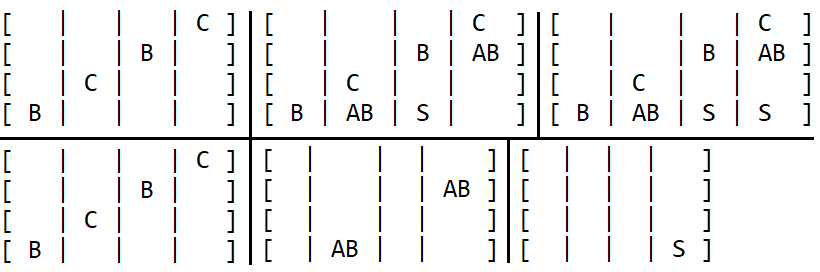
\includegraphics[width=0.9\textwidth]{obrazky-figures/comparisionOfTables.png}
	\caption{Porovnanie vypĺňania obsahov tabuliek algoritmov CYK. Prvý riadok obsahuje tabuľky pre algoritmus CYK pre bezkontextové gramatiky. Druhý obsahuje tabuľky modifikácie algoritmu CYK pre E0L systémy.}
	\label{compareTables}
\end{figure}

%---------------------------------------------------------------------------------
\subsection*{ET0L systémy}
Pri tejto modifikácii algoritmu \textit{CYK} budeme vychádzať z už popísanej modifikácie pre E0L systémy (viď \ref{EOL parsing}). Nad modifikáciou pre E0L systémy zapracovať spracovanie pre viaceré tabuľky pravidiel, ktorými sa vyznačujú ET0L systémy.

Tabuľky, alebo ináč povedané množiny pravidiel, rozvetvujú spracovanie syntaktickou analýzou. Pri každom kroku môže byť použitá ľubovoľná tabuľka. To znamená, že algoritmus sa musí nutne rozvetvovať kvôli rôznym postupnostiam výberu tabuliek. Musia byť skontrolované všetky kombinácie výberu tabuliek v jednotlivých krokoch. 

O tomto probléme sa dá povedať, že je to \textit{prehľadávanie stavového priestoru}, ktorým sa zaoberá umelá inteligencia. V skratke ide o to, že musíme nájsť takú postupnosť operátorov, aby sme sa dopracovali ku konečnému stavu. Operátory v našom prípade môžeme chápať ako tabuľku pravidiel a konečný stav je tabuľka CYK, ktorá na pozícii [1, n] obsahuje počiatočný symbol. Teda úspešné ukončenie algoritmu.

\subsubsection*{Backtracking}
Jednou z metód riešenia problému prehľadávania stavového priestoru je práve backtracking. Jedná sa o neinformovanú metódu, nemá teda žiaden spôsob ako jednotlivé stavy ohodnotiť \cite{IZU}. To nám pre túto modifikáciu algoritmu CYK vyhovuje, pretože by bolo obtiažne, ak vôbec možné, vhodne ohodnotiť stav tabuľky CYK.

Backtracking namiesto expanzie vybraného uzlu(stavu) vygeneruje iba jedného následníka. Expanzia uzlu by v našom prípade znamenala aplikáciu všetkých tabuliek na~aktuálnu tabuľku CYK a získanie $n$ nových tabuliek CYK, kde $n$ je počet tabuliek pravidiel.

Pri nájdení nevyhovujúceho stavu sa metóda backtrackingu vráti na predchádzajúci stav a vygeneruje sa ďalší nasledovník. Pokiaľ sa už žiaden nový nasledovník vygenerovať nedá, metóda sa vracia o krok späť, pokiaľ je to možné \cite{IZU}.


\subsection*{Popis fungovania}
Backtracking je docielený rekurzívnym spustením ďalšieho kroku pre každú existujúcu tabuľku. Na začiatku kroku je nastavená tabuľka, ktorá sa v danom kroku bude používať. Na konci kroku sa znova rekurzívne spustia kroky pre všetky existujúce tabuľky pravidiel. Keďže prvý krok nemôže byť spustený predchádzajúcim, sú všetky prvé kroky spustené po naplnení diagonály neterminálmi. Veľmi dôležité je aj samotné napĺňanie diagonály neterminálmi. Keďže existuje viacero tabuliek pravidiel, je potrebné naplniť diagonálu pomocou každej z nich. Tento popis je podrobne popísaný pomocou pseudokódu \ref{CYKET0L}.

Týmto spôsobom získavame backtracking nad aplikáciou všetkých možných kombinácii tabuliek pravidiel v jednotlivých krokoch.

\begin{algorithm}
\caption{Cocke-Younger-Kasami algoritmus syntaktickej analýzy pre ET0L systémy}
\label{CYKET0L}

\textbf{Input}
\setlist{nolistsep}
\begin{itemize}[noitemsep]
    \item ET0L system, \(E = (\Sigma, T, P^T, w_o))\) in normal form \ref{E0LNormalForm}
    \item \(w = a_1a_2...a_n\)  where  \(a_i \in {}_E\Delta, 1 \leq i \leq n \), for some \(n \geq 1\).
\end{itemize}
\textbf{Output} 
\begin{itemize}[noitemsep]
    \item \textbf{ACCEPT} if \(w \in L(G)\)
    \item \textbf{REJECT} if \(w\notin L(G)\)
\end{itemize}
\textbf{Method}
\begin{algorithmic}
\For{$\forall P \in P^T$}
\State $ CYK[i,j] = \varnothing$ for $1 \leq i \leq j \leq n $

\For{i = i \textbf{to} $n$}
    \If{$ A \rightarrow a_i \in P $}
        \State $add\ A\ to\ CYK[i,i]$
    \EndIf
\EndFor
\For{$\forall X \in {}_ET$}
\State \Call{CYKCycle}{CYK, P, $\varnothing$}
\EndFor
\EndFor

\State \textbf{REJECT}
\\
\Function{CYKCycle}{CYK, P, history}
\State $ CYKNext[i,j] = \varnothing$ for $1 \leq i \leq j \leq n $
\State $ empty\ is\ set\ of\ terminals,\ \forall A \in empty, A \Rightarrow^* \epsilon\ and\ A \in \Sigma / T$

\Repeat

\If{$ A \in CYK[i,j], \alpha \rightarrow A \in P $ for some $A, \alpha \in \Sigma$}
\State
\State $add\ \alpha\ to\ CYKNext[i,j]$
\EndIf

\If{$ B \in CYK[i,j], C \in empty, A \rightarrow BC \lor A \rightarrow CB \in P $ for some $A,B,C \in \Sigma / T$ \phantom{xxxxx}}
\State $add\ A\ to\ CYKNext[i,j]$
\EndIf

\If{$ B \in CYK[i,j], C \in CYK[j+1,k], A \rightarrow BC \in P $ for some $A,B,C \in \Sigma/T$}
\State $add\ A\ to\ CYKNext[i,k]$
\EndIf
\Until{no changes}

\If{$(CYKNext, empty) \in history$}
    \State \textbf{return}
\Else
    \State $add\ (CYKNext, empty)\ to\ history$
\EndIf

\If{No new reduction in this step}
\State \Return
\EndIf
\If{$ S \in CYKNext[1,n] $}
    \State \textbf{ACCEPT}
\Else
    \State $ CYK = CYKNext$
    \For{$\forall R \in P^T$}
        \State \Call{CYKCyklus}{CYK, R, history}
    \EndFor
\EndIf


\EndFunction

\end{algorithmic}
\end{algorithm}

\section{Algoritmus zhora-dole pre ET0L systémy}
\label{top-downET0L}
Prístup syntaktickej analýzy zhora-dole predstavuje opačný prístup ako zdola-hore, ktorý je využívaný v algoritme CYK a aj v jeho navrhovaných modifikáciách.

Nevýhodou tohto prístupu je väčšia časová zložitosť, nakoľko v najhoršom prípade musíme vygenerovať všetky možné slová o danej dĺžke. To však predstavuje aj výhodu, pretože je možné tento algoritmus použiť na všetky možné slová o danej dĺžke. Ďalšou výhodou je, že pravidlá môžu byť v ľubovoľnom tvare.

\subsection*{Riešenie nedeterminizmu a paralelizmu}
Jedným z dvoch hlavných problémov pre tento druh syntaktickej analýzy sú nedeterministické pravidlá, to znamená, že jeden symbol sa vyskytuje na ľavej strane viacerých pravidiel. Ináč povedané, existuje možnosť, že sa môže prepísať na viacero rôznych reťazcov. Riešením tohto problému je rekurzia. Pri každej aplikácii pravidla sa použitím rekurzie zaistí, že sa vygenerovali všetky možnosti aplikácii rôznych pravidiel pre~prepisovaný symbol.

Druhým problémom je zaistiť paralelizmus prepisovania. Problém je to preto, lebo tento paralelizmus potrebujeme docieliť pomocou sekvencie akcií. Musíme teda napodobniť paralelizmus sekvenčne. To je dosiahnuté zavedením indexu ukazujúceho na symbol, ktorý má byť prepísaný ako ďalší. Pokiaľ index neukazuje na začiatok slova, tak na toto slovo neboli aplikované všetky potrebné pravidlá, derivačný krok teda stále prebieha.

\subsection*{Popis fungovania}
Máme určené počiatočné slovo, na ktoré budú aplikované derivačné kroky. Na začiatku je index nastavený na 0 (v rámci tohto algoritmu uvažujeme indexovanie od 0), čiže na index prvého symbolu slova.

Existuje funkcia, ktorá slúži na aplikáciu individuálnych pravidiel. Keďže sú ET0L systémy plne paralelné, musia sa aplikovať pravidlá na všetky symboly slova súčasne, nejde o~kompletný derivačný krok. Funkcia ako parametre prijíma reťazec, index a aktuálnu tabuľku pravidiel (keďže sa jedná o ET0L systémy).

Táto funkcia na aplikáciu pravidiel aplikuje z tabuľky symbolov všetky existujúce pravidlá na symbol, na ktorý ukazuje index. Tento index je prepočítaný podľa pravidla, ktoré sa aplikovalo. Zvýši (posunie) sa o dĺžku pravej strany aplikovaného pravidla. Ukazuje na ďalší symbol pôvodného slova. Pokiaľ bolo pravidlo aplikované na posledný symbol, index sa vracia na začiatok slova, teda na nulu.

Po tom ako funkcia aplikuje pravidlo a prepočíta index, rekurzívne zavolá sama seba s~týmito novými hodnotami. V prípade, že je nový index nulový, znamená to, že bol dokončený celý derivačný krok. Preto funkcia navyše rekurzívne zavolá samú seba pre každú tabuľku pravidiel, ktorú daný ET0L systém obsahuje.

Samozrejme sa na začiatku tejto funkcie musia kontrolovať slová, ktoré funkcia prijala ako parameter. To slúži ako ukončovacia podmienka tejto rekurzie. Jednou je, že sme dosiahli slovo, ktoré kontrolujeme. V tom prípade algoritmus končí \textbf{úspechom}. Druhou je, že prijaté slovo je dlhšie, než dĺžka kontrolovaného slova. Ak algoritmus skončí bez toho, aby bolo vygenerované vyhľadávané slovo, algoritmus končí neúspechom.

Tento algoritmus je v ekvivalentnej forme zapísaný pomocou pseudokódu \ref{topDownET0L}.

\subsubsection*{Generátor slov}
Pokiaľ algoritmus mierne modifikujeme, je pomocou neho možné vygenerovať všetky možné slová o istej maximálnej dĺžke z jazyka, ktorý je generovaný daným ET0L systémom.

Pokiaľ je počas syntaktickej analýzy vygenerované slovo, ktoré obsahuje len neterminály a má správnu dĺžku, pridá sa do množiny vygenerovaných slov. Je nutné zrušiť kontrolu úspešnosti. Tá by nastala v prípade, že slovo vygenerované syntaktickou analýzou je rovnaké ako kontrolované slovo. Pokiaľ by táto kontrola nebola zrušená, neboli by vygenerované žiadne slová, ktoré by boli vygenerované po kontrolovanom slove.


\begin{algorithm}
\caption{Algoritmus syntaktickej analýzy ET0L systémov zhoda-dole}
\label{topDownET0L}

\textbf{Input}
\setlist{nolistsep}
\begin{itemize}[noitemsep]
    \item ET0L system, \(E = ({}_E\Sigma, {}_ET)\)
    \item \(w = a_1a_2...a_n\)  where  \(a_i \in {}_E\Delta, 1 \leq i \leq n \), for some \(n \geq 1\).
\end{itemize}
\textbf{Output} 
\begin{itemize}[noitemsep]
    \item \textbf{ACCEPT} if \(w \in L(G)\)
    \item \textbf{REJECT} if \(w\notin L(G)\)
\end{itemize}
\textbf{Method}
\begin{algorithmic}
\For{$\forall R \in {}_ET$}
    \State \Call{applyRule}{$w_o, 0, R$}
\EndFor

\State \textbf{REJECT}
\Comment{No recursive call of ApplyRule accepted}
\\
\Function{applyRule}{word, index, ruleSet}
\If{$word = w$}
    \State $ACCEPT$
\EndIf

\If{$|word| > |w|$}
    \State \Return
\EndIf

\For{$\forall R \in ruleSet$ where $word[index] \to x, x \in {}_\Sigma$}
    \State $newWord$ = replace $word[index]$ with $x$ in $word$
    \State $newIndex$ = $index + |x|) \mod |newWord|$
    \If{$newIndex == 0$}
        \For{$\forall R \in {}_ET$}
        \Comment{derivation step complete, use all tables recursively}
            \State \Call{applyRule}{newWord, newIndex, R}
        \EndFor
        \State \Call{applyRule}{newWord, newIndex, ruleSet}
        \Comment{derivation step is not complete}
    \EndIf
\EndFor
\EndFunction
    
\end{algorithmic}
\end{algorithm}

\subsection*{Verzia pre E0L systémy}
Tento algoritmus je možné aplikovať aj pre E0L systémy. Tie sú vlastne špeciálnym typom ET0L systémov, ktoré majú len jednu tabuľku. Preto je tento algoritmus použiteľný pre~E0L systémy.

\subsection*{Verzia pre bezkontextové gramatiky}
Algoritmus je možné upraviť pre bezkontextovú gramatiku nasledovne. Odstráni sa indexácia v rámci slova. Rekurzívne volanie funkcie sa vykoná pre každý symbol v slove. Takto získame algoritmus pre generovanie slov bezkontextových gramatík.

\subsection*{Nedostatok návrhu}
Navrhnutý algoritmus obsahuje nedostatok pri práci s prázdnymi prepisovacími pravidlami. Ten zamieta vygenerované slová, ktoré sú dlhšie než kontrolované slovo. Aplikáciou prázdnych prepisovacích pravidiel je však možné získať 
z dlhšieho slova kratšie.

Možným riešením je využitie množiny $empty$ podobne ako pri modifikáciách algoritmu CYK. Do dĺžky slova by neboli započítané prvky tejto množiny pretože by mohli byť zmazané. Toto riešenie však nie je možné použiť. Ako príklad uvažujme prepisovacie pravidlá $S \to A$, $A \to AA$, $A \to a$, $A \to \epsilon$. Ľubovoľne dlhý reťazec o dĺžke $n$ neterminálov $A$ je možné jedným paralelným derivačným krokom získať reťazec o dĺžke $\leq n$. Preto by mohli byť pomocou algoritmu generované nekonečné dlhé slová.

%=============================================================================================
\chapter{Implementácia}
\label{implementation}

V predchádzajúcej kapitole boli predstavené a popísané dve metódy syntaktickej analýzy pre ET0L systémy. Prvá z nich pracuje na princípe syntaktickej analýzy zdola-hore (viď \ref{analysysTypes}), teda z pôvodného slova sa spätne redukciou pravidiel vracia k počiatočnému symbolu. Táto metóda vychádza z algoritmu Cocke-Younger-Kasami a pomocou jeho modifikácie získavame algoritmus, ktorý funguje pre syntaktickú analýzu ET0L systémov.

Druhou variantou je algoritmus na princípe zhora-dole, snaží sa teda vygenerovať dané slovo aplikáciou pravidiel na počiatočné slovo.

\section{Návrh implementácie}
Tieto metódy syntaktickej analýzy je potrebné implementovať v rámci aplikácie. Ako aplikáciu som zvolil konzolové rozhranie, ktoré spúšťa a interaguje s jednotlivými algoritmami. Jedná sa o rozhranie, pomocou ktorého je možné vybrať konkrétny algoritmus. Pomocou tohto algoritmu sa vykoná syntaktická analýza.

Keďže sa jedná o konzolovú aplikáciu, všetky potrebné voľby a parametre sú špecifikované pomocou parametrov predaných cez konzolové rozhranie.

Metódy syntaktickej analýzy, ktoré boli špecifikované pre ET0L systémy, boli vytvorené aj pre bezkontextové gramatiky a E0L systémy, pretože na seba naväzujú. Každý tento algoritmus je implementovaný pomocou samostatného skriptu.

\section{Implementačný jazyk}
Pred samotnou implementáciou bolo potrebné zvoliť vhodnú platformu implementácie.

Zvolil som programovací jazyk \textbf{Python} vo verzii 3.7 . Jedná sa o vysokoúrovňový objektovo orientovaný programovací jazyk. Poskytuje vysokú mieru abstrakcie nad jednotlivými konštruktmi ktoré obsahuje spoločne s bohatou štandardnou knižnicou. Pomocou jazyka Python preto možný rýchly vývoj. Vďaka týmto pozitívam sa hodí na~implementáciu algoritmov definovaných v tejto práci.

Hlavnou nevýhodou jazyka Python je, že sa jedná o interpretovaný jazyk. Na jeho spustenia teda musíme mať nainštalovaný interpret. Vo všeobecnosti sú interpretované jazyky pomalšie, čo platí aj pre Python. Pre túto prácu to však nepredstavuje problém.


\section{Štruktúra aplikácie}
Každá implementácia jednotlivých algoritmov je tvorená triedou v samostatnom súbore. Keďže boli navrhnuté dve metódy syntaktickej analýzy a je implementovaná verzia pre~bezkontextové gramatiky, E0L a ET0L systémy, existuje 6 tried syntaktických analýz.

Pre prácu algoritmov syntaktickej analýzy je potrebný vstupný formálny model, teda gramatika alebo L-systém. Najdôležitejšou časťou tohto vstupného modelu sú prepisovacie pravidlá. Vďaka forme týchto pravidiel a ich potencionálnej dĺžke bola vytvorená trieda, ktorá tieto pravidlá získava zo súboru. Existujú dve implementácie tejto triedy. Pri ET0L systémoch je potrebné rozdeliť pravidlá do viacerých tabuliek a preto je potrebné vhodne upraviť implementáciu.

Užívateľské rozhranie aplikácie tvorí skript, ktorý pomocou konzolového rozhrania prijíma od užívateľa potrebné informácie pre spustenie jednotlivých syntaktických analýz.

\section{Rozhranie aplikácie}
Ako rozhranie pre interakciu užívateľa s jednotlivými algoritmami syntaktickej analýzy bolo zvolené konzolové rozhranie. Pomocou konzolových parametrov užívateľ programu poskytuje informácie, ktoré sú potrebné k správnemu fungovaniu. 

Konzolové parametre sú: 

\begin{itemize}
    \item[] -h, (help) vypísanie nápovedy pre správne používanie aplikácie
    \item[] -C | E | T , výber verzie algoritmu pre bezkontextové gramatiky, E0L alebo ET0L systémy v tomto poradí
    \item[] -r <rules>, špecifikovanie súboru v ktorom sa nachádzajú prepisovacie pravidlá. Forma pravidiel je podrobne popísaná v časti \ref{ruleFormat}
    \item[] -w <word>, špecifikovanie slova, ktoré má byť spracované pomocou syntaktickej analýzy
    \item[] --top-down, použitie algoritmov založených na princípe zhora dole
    \item[] --start-word <axiom>, definovanie $axiomu$ pre algoritmus na princípe zhora dole. Východzia hodnota je \uv{S}
    
\end{itemize}

\section{Načítanie prepisovacích pravidiel}
Každá implementácia algoritmov syntaktickej analýzy potrebuje mať nejakým spôsobom definované prepisovacie pravidlá. Či už to je napevno naprogramované v kóde, alebo sú tieto pravidlá načítané dynamicky.

V tejto aplikácii sa pravidlá načítavajú zo špecifikovaného súboru obsahujúceho tieto pravidlá. Je potrebné vhodne načítať tabuľky pravidiel pre ET0L systémy. Preto existujú dve implementácie triedy \textbf{\texttt{RuleReader}}, ktorá implementuje načítanie pravidiel zo súboru.

\subsection*{Formát súboru s pravidlami}
\label{ruleFormat}
Prepisovacie pravidlá, ktoré potrebujú algoritmy syntaktickej analýzy, musia byť uložené v~samostatnom súbore. Tento súbor môže mať ľubovoľný názov, ktorý sa predáva aplikačnému rozhraniu.

Každé pravidlo musí byť na samostatnom riadku a spĺňať nasledovný formát:
\[\text{s--->s${}^+$ alebo s--->-}, \quad\quad \text{kde s je ľubovoľné písmeno}\]

To znamená, že prepisovaný znak, teda písmeno na ľavej strane, môže byť len jedno, keďže všetky navrhnuté algoritmy sú bezkontextové. Na pravej strane pravidla, teda reťazec, ktorým sa prepíše znak na ľavej strane, môže pozostávať z jedného alebo viacerých písmen, veľkých aj malých. Ľavé a pravé strany pravidiel sú od seba oddelené znakmi \uv{-} a \uv{>}, ktoré spoločne tvoria šípku.

Pri vytváraní objektu triedy \texttt{RuleReader} je potrebné konštruktoru predať názov súboru, z ktorého sa majú pravidlá načítať.

\subsubsection*{Oddelenie tabuliek pravidiel pre ET0L systémy}
ET0L systémy umožňujú používanie viacerých množín prepisovacích pravidiel, ktoré sa nazývajú tabuľky. Preto je potrebné tieto tabuľky vo vstupnom súbore s pravidlami vymedziť. Jednotlivé tabuľky sú od seba oddelené pomocou znaku \textbf{\uv{\#}} na samostatnom riadku.

\subsubsection*{Kontrola formátu pravidiel}
Pri načítaní pravidiel zo súboru sú tvary pravidiel kontrolované pomocou \textit{RegEx}-ov, čo je implementácia regulárnych výrazov popísaných v časti \ref{regularExpression}.

V prípade používania algoritmov založených na algoritme Cocke-Younger-Kasami (ďalej len CYK), pravidlá musia byť v správnej normálovej forme (\ref{E0LNormalForm}). Táto podmienka je taktiež kontrolovaná pomocou \textit{RegEx-ov}.
\\\\
Pri načítaní vstupného súboru sa ignorujú netlačiteľné (white-space) znaky.

\subsection*{Reprezentácia prepisovacích pravidiel}
Pre vnútornú reprezentáciu prepisovacích pravidiel sa používa dátová štruktúra slovník (anglicky dictionary), ktorá sa taktiež nazýva hašovacia tabuľka (anglicky hash-table). Táto štruktúra umožňuje zaviesť indexáciu pomocou vlastných kľúčov, ktoré slúžia na~indexovanie. V implementácii sa ako kľúče využívajú ľavé strany pravidiel, teda symboly, ktoré sa majú prepísať. Hlavnou výhodou tejto dátovej štruktúry je rýchly prístup k dátam a jednoduchosť používania.

Slovník pre každý kľúč, teda ľavú stranu pravidla, uchováva zoznam pravých strán pravidiel, ktoré predstavujú reťazce, ktorými sa môže daná ľavá strana pravidla prepísať. Pravé strany pravidiel pre konkrétnu ľavú stranu musia byť ukladané v zozname, keďže množina pravidiel nemusí byť deterministická a môže tak obsahovať viacero pravých strán pre tú istú ľavú stranu pravidiel.

Pre získanie pravidiel slúži metóda triedy \texttt{RuleReader} nazvaná \texttt{getRulesDictionary}, ktorá prijíma parameter rozhodujúci o tom, či majú byť pravidlá kontrolované pre vhodnú normálovú formu.

Implementácia triedy \texttt{RuleReader} pre jednu množinu pomocou metódy \texttt{getRulesDictionary} má ako návratovú hodnotu slovník pravidiel. V prípade implementácie pre viacero tabuliek pravidiel používanej pre ET0L systémy, je návratová hodnota zoznam slovníkov pravidiel.

\section{Syntaktická analýza}
Oba spôsoby syntaktickej analýzy navrhnutej v kapitole \ref{syntax} sú implementované ~bezkontextové gramatiky, E0L a ET0L systémy. Jednotlivé implementácie sú tvorené triedou a metódou \texttt{parse}, ktorá prijíma ako parameter reťazec určený pre syntaktickú analýzu.

\subsubsection*{Reprezentácia formálnych modelov}
Modely, s ktorými pri syntaktickej analýze pracujeme sú bezkontextové gramatiky, E0L a ET0L systémy. Síce ide o tri rozdielne formálne modely, sú ale definované rovnakými základnými vlastnosťami. Jedná sa o abecedu terminálov a neterminálov, prepisovacie pravidlá a počiatočný symbol, prípadne slovo.

Definícia prepisovacích pravidiel už bola popísaná skôr v tejto kapitole. Abeceda terminálov a neterminálov nie je definovaná explicitne. Nie je to potrebné, stačí, že sú použité v rámci prepisovacích pravidiel. Predpokladá sa, že veľké písmená reprezentujú neterminály a malé písmená zasa terminály. Takáto reprezentácia je v rámci teoretickej informatiky bežne používaná. $\epsilon$ na pravej strane prepisovacieho pravidla je reprezentovaný pomocou pomlčky (\uv{-}).

Bezkontextové gramatiky majú vo svojej definícii počiatočný symbol, E0L a ET0L systémy takzvaný \textit{axiom}, počiatočné slovo. Všetky implementácie týchto formálnych modelov založené na algoritme CYK predpokladajú ako počiatočný symbol alebo axiom neterminál \uv{S}. Implementácie algoritmov založených na princípe zhora-dole pre E0L a ET0L sytémy ako axiom implicitne používajú neterminál \uv{S}. Pomocou parametra \texttt{startWord} funkcie \texttt{parse} je však možné použiť ľubovoľný reťazec obsahujúci len terminály a neterminály. To však neplatí pre verziu pre bezkontextové gramatiky. Tam je počiatočný symbol vždy \uv{S}.


\subsubsection{Obmedzenia rekurzie}
Algoritmy syntaktických analýz pre ET0L systém využívajú vo svojom návrhu rekurziu. Algoritmy sú však výpočetne náročný a pri použití rekurzie mal príliš veľkú hĺbku zanorenia. To znamená, že funkcia príliš veľa krát zavolala sama seba bez toho, aby sa navrátila z tohto vnorenia. Preto pri využití rekurzie nastali dva problémy. Prvým je, že algoritmy boli príliš pomalé. Druhým je obmedzenie jazyka Python na maximálnu hĺbku rekurzie, ktorá bola prekročená. Dôsledkom toho bol program zastavený a systémom automaticky ukončený.

\subsubsection{Prevod rekurzívnej funkcie do iteratívnej formy}
Riešením problémov spojených s rekurziou je prevod rekurzívnej funkcie na iteratívnu. Pre~parametre takejto funkcie sa vytvoria zásobníky a vložia sa do nich počiatočné hodnoty.  Obsah funkcie sa zabalí do cyklu, ktorý sa vykonáva, kým nie sú zásobníky prázdne. Na~začiatku cyklu sa vyberú hodnoty z vrcholov zásobníkov. Rekurzívne volanie funkcie sa nahradí vložením hodnôt parametrov do zásobníkov. Vďaka tomu je rekurzívna funkcia konvertovaná na iteratívnu.

\subsection{Syntaktická analýza založená na Cocke-Younger-Kasami algoritme}


Triedy \texttt{CFGParserCYK}, \texttt{E0LParserCYK}, \texttt{ET0LParserCYK} sú implementácie navrhnutých algoritmov pre syntaktickú analýzu v kapitole \ref{syntax} pomocou modifikácie algoritmu Cocke-Younger-Kasami pre bezkontextové gramatiky (viď \ref{CYK}). Pseudokód fungovania týchto implementovaných tried je popísaný v algoritmoch \ref{CYKBKG} pre bezkontextové gramatiky implementovaný v triede \texttt{CFGParserCYK}, \ref{CYKE0L} pre E0L systémy implementovaný v triede \texttt{ET0LParserCYK} a \ref{CYKET0L} pre E0L systémy implementovaný v triede \texttt{ET0LParserCYK}.


\subsubsection*{Vnútorná reprezentácia tabuliek algoritmu CYK}
Tieto tabuľky slúžia pre uchovávanie stavu symbolov počas algoritmu CYK. Jedná sa o~dvojrozmerné pole symbolov. Dátový typ jednotlivých položiek tabuľky je \texttt{množina}, v~jazyku Python reprezentovaná pomocou \texttt{set()}. Tento dátový typ je nezoradený a vždy obsahuje len unikátne hodnoty. To je výhodné, nakoľko duplicitné hodnoty sú v týchto tabuľkách zbytočné. Vďaka využitiu tohto dátového typu nie je potrebné túto duplicitu riešiť.

\subsubsection*{Formátovanie výpisu tabuliek algoritmu CYK}
Na konci každého kroku týchto algoritmov je do konzoly vypísaný aktuálny stav tabuľky CYK. Funkcia \texttt{print()}, ktorá v jazyku Python slúži na výpis do konzoly, dokáže spracovať aj dvojrozmerné polia, akým sú aj tabuľky používané algoritmom CYK. Tento výpis však nie je užívateľsky prívetivý a zle sa v ňom orientuje.

Každá trieda obsahuje funkciu na výpis týchto tabuliek, nazvanú \texttt{printTable}. Tá invertuje tabuľku podľa osy Y, takže index $[0, 0]$ je v ľavom spodnom rohu. Taktiež zabezpečí, že šírka stĺpca je určená podľa najdlhšej množiny symbolov v danom stĺpci. Vďaka tomu sú tabuľky vypísané do konzoly pre užívateľa ľahko pochopiteľné. Príklad výpisu tabuľky je možné vidieť na obrázku \ref{tableExample}.

\begin{figure}[hbt]
	\centering
	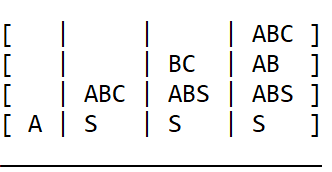
\includegraphics[width=0.4\textwidth]{obrazky-figures/exampleTable.png}
	\caption{Ukážka výpisu tabuľky algoritmu Cocke-Younger-Kasami. Formátovanie šírky stĺpcov je určené podľa najširšej bunky daného stĺpca.}
	\label{tableExample}
\end{figure}

\subsubsection*{Výstup algoritmu}
Triedy \texttt{CFGParserCYK} a \texttt{E0LParserCYK} priebežne vypisujú aktuálnu tabuľku $CYK$ na~štandardný výstup. To však nie je vhodné pre triedu \texttt{ET0LParserCYK}, nakoľko by bol tento výpis kvôli prehľadávaniu správnej kombinácie tabuliek neprehľadný. Vypíše sa len postupnosť tabuliek, ktorá viedla k~úspešnosti syntaktickej analýzy. Ak analýza úspešná nebola, nevypíše sa nič. Metóda \texttt{parse} pri úspechu syntaktickej analýzy vracia hodnotu \texttt{True}, ináč \texttt{False}. To platí pre všetky triedy.

Pred vypisovaním samotných tabuliek je vypísané slovo, ktoré bude syntaktická analýza spracovávať.

\subsubsection*{Nedostatky implementovaného algoritmu}
Pri implementácii bol objavený nedostatok tohto algoritmu pri používaní komplikovaných prepisovacích pravidiel, ktoré obsahujú aj prázdne prepisovacie pravidlá. Implementácia verzie tohto algoritmu pre ET0L systémy bola pomalá pre správne aj nesprávne slová. V niektorých prípadoch trvala jednotky sekúnd. Jednoduchou zmenou vyberania hodnôt zo zásobníkov bolo možne tento problém odstrániť aspoň pre správne slová. Hodnoty sa nevyberajú z vrcholu zásobníku ale z jeho spodku. Tým sa zásobník mení na frontu. Problém s rýchlosťou pre neplatné slová zostáva.

\subsection{Syntaktická analýza zhora-dole}
\label{topDownImplementation}
Implementované algoritmy pre jednotlivé formálne modely sú popísané v časti \ref{top-downET0L}. Trieda \texttt{TopDownCFGParser} je implementáciou verzie algoritmu syntaktickej analýzy pre~bezkontextové gramatiky, \texttt{TopDownE0LParser} pre E0L systémy a \texttt{TopDownET0LParser} pre ET0L systémy.


\subsubsection*{Generovanie slov}
Jednoduchou úpravou tejto syntaktickej analýzy je možné vygenerovať všetky slová patriace do jazyka, ktorých dĺžka je menšia alebo rovná $n$, pričom $n \geq 1$. Pri nedodržaní tejto podmienky nebude nikdy vygenerované žiadne slovo.

Metóda \texttt{generateValidWords} slúži na vygenerovanie týchto slov. Tá interne využíva rovnakú metódu, ako metóda syntaktickej analýzy \texttt{parse}. Ak je počas generácie získané platné slovo, pridá sa do množiny \texttt{generatedWords}, ktorá obsahuje vygenerované slová. Vygenerované slová môžu byť použité pre testovanie syntaktickej analýzy založenej na~algoritme CYK.

Pomocou metódy \texttt{generateAllCombinations} vygeneruje všetky možné kombinácie terminálov, ktorých dĺžka je menšia alebo rovná $n$. Vygenerované kombinácie môžu byť rozdelené na dva disjunktné množiny. Jednou sú slová patriace do generovaného jazyka a~druhou sú tie, ktoré do neho nepatria.

Pokiaľ je vykonaný rozdiel množín, kde od všetkých kombinácii terminálov odčítame reťazce generované jazykom, získame množinu slov ktoré do generovaného jazyka nepatria. Takáto množina má využitie pri testovaní.

\subsubsection{Výstup algoritmu}
Metóda \texttt{parse} pri úspechu syntaktickej analýzy vracia hodnotu \texttt{True}, ináč \texttt{False}. To platí pre všetky triedy.

Metódy \texttt{generateValidWords} a \texttt{generateAllCombinations} vracajú množiny.

%=============================================================================================
\chapter{Testovanie}
\label{testovanie}
Na testovanie softvéru sa niekedy vynakladá viac zdrojov než na samotnú implementáciu. Platí to hlavne v prípade, kedy chyba daného softvéru môže spôsobiť veľké škody, napríklad pád lietadla.

Testovaniu sa v rámci tejto práce nebudeme venovať do hĺbky, nakoľko sa jedná o veľmi komplexnú tematiku. Rozdelenie druhov testov môže byť niekedy neurčité, pojmy sa môžu prekrývať, alebo môžu byť úplne zamenené.

V rámci tejto práce testujeme funkčnosť tried syntaktických analýz ako celkov.

\section{Rozhranie testov}
Skript pre samotné vykonanie testov je implementovaný v súbore \texttt{parserTest.py}. Nie je využívaná žiadna knižnica poťažmo framework pre testovanie. To prebieha vytváraním objektov tried syntaktických analýz a kontrolovaním výsledku spustenia funkcie \texttt{parse}.


\subsection*{Testovacie vstupy}
Pri spúšťaní syntaktických analýz je potrebné im predať isté vstupné hodnoty. Konkrétne súbor s prepisovacími pravidlami a slovo, ktoré sa má kontrolovať.

Za účelom tohto testovania bol vytvorený samostatný súbor s prepisovacími pravidlami, ktorý je v rámci testovania používaný. Tento súbor s prepisovacími pravidlami obsahuje všetky možnosti vlastností prepisovacích pravidiel, ktoré sa v rámci syntaktickej analýzy chovajú odlišne.

Vstupné slová sú generované syntaktickou analýzou zhora dole. Triedy týchto analýz obsahujú metódu \texttt{generate}, ktorá vracia dvojicu \texttt{touple} množín. Prvá množina obsahuje všetky slová patriace do generovaného jazyka o maximálnej dĺžke $n$, pričom $n$ je parameter metódy \texttt{generate}. Druhá množina obsahuje všetky platné slová o dĺžke $n$, ktoré však nepatria do generovaného jazyka.

Vďaka tomu, že generujeme aj všetky slová, ktoré nepatria do generovaného jazyka, sú vylúčené takzvané \textit{false positives}. Tento výraz znamená, že test prebehol úspešne aj keď nemal. Ako názornú ukážku uvažujme algoritmus syntaktickej analýzy, ktorý prijme všetky slová, aj keď nepatria do generovaného jazyka. Pri jeho testovaní len pomocou slov patriacich do generovaného jazyka by testy mali 100\%-nú úspešnosť. Pokiaľ by boli testované slová, ktoré majú byť odmietnuté, úspešnosť testov by bola 0\%. Vďaka týmto testom by sme zistili, že algoritmus je nefunkčný.

\subsection{Zohľadnenie nedostatkov algoritmov}
Testované syntaktické analýzy obsahujú dva problémy. Modifikácia algoritmu CYK pre~ET0L systémy je pomalá pri existencii prázdnych prepisovacích pravidiel a následnej kontrole neplatných slov. Algoritmy založené na princípe zhora-dole zasa odmietajú niektoré slová, ktoré by mohli byť aplikáciou prepisovacích pravidiel skrátene na požadovanú dĺžku a následne prijaté. To by znamenalo, že by boli pri generovaní vstupných slov označené ako~neplatné.

Pri testovaní nesprávnych slov sú použité také prepisovacie pravidlá, ktoré neobsahujú prázdne prepisovacie pravidlá.

\subsection*{Testované analyzátory}
Generácia vstupných slov pre testovanie prebieha pomocou syntaktických analýz zhora-dole. Táto funkcionalita je popísaná v časti \ref{topDownImplementation}. Preto nie je dôvod pomocou týchto vstupov tieto analýzy testovať. Testované sú len syntaktické analyzátory založené na algoritme Cocke-Younger-Kasami.

Vyplýva však otázka, ako si môžeme byť istý, že syntaktická analýza zhora-dole funguje správne. Táto syntaktická analýza je nepriamo testovaná pomocou testov syntaktickej analýzy CYK. Pokiaľ oba tieto druhy syntaktickej analýzy prijímajú a odmietajú rovnakú množinu slov pre konkrétny formálny model, je nepravdepodobné, že sú obe chybné.

\subsection*{Výstup testovania}
Po spustení testov sa všeobecne očakáva istý výstup, ktorý informuje o úspešnosti jednotlivých testov. V prípade neúspešnosti niektorých, prípadne všetkých testov, musí byť z výstupu jasné, ktoré testy prebehli neúspešne. Dôležitou informáciou je taktiež koľko testov z celkového počtu spustených testov prebehlo úspešne.

Pri testovaní v rámci tejto práce je výstup vypísaný na štandardný výstup. Pre každú testovanú syntaktickú analýzu sú vždy vypísané počty úspešne spracovaných slov, ktoré patria do generovaného jazyka. Taktiež sú vypísané počty úspešne spracovaných slov, ktoré nepatria do generovaného jazyka.

V prípade, že syntaktická analýza nesprávne spracuje vstupné slovo, je táto informácia vypísaná na štandardný vstup spolu s daným slovom.

Príklad tohto výstupu je možné vidieť na obrázku \ref{testOutput}. Pri tomto testovaní bola pre~názornosť do testovacieho skriptu schválne zavedená chyba.

\begin{figure}[hbt]
	\centering
	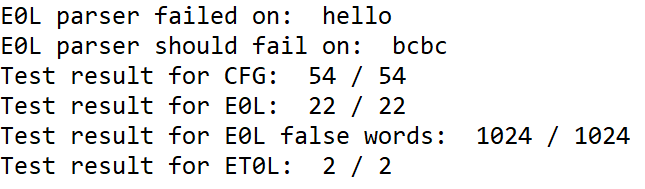
\includegraphics[width=0.6\textwidth]{obrazky-figures/testOutput.png}
	\caption{Príklad výstupu testovacieho skriptu. Do testovacieho skriptu bola zámerne zavedená chyba. Syntaktická analýza pre E0L systémy odmietla slovo \texttt{hello}, ktoré mala podľa testov prijať. Naopak, prijala slovo \texttt{bcbc}, ktoré mala podľa testov odmietnuť.}
	\label{testOutput}
\end{figure}

\subsubsection*{Blokovanie štandardného vstupu}
Syntaktická analýza založená na algoritme CYK počas svojho spustenia produkuje textový výstup na štandardný výstup. Táto vlastnosť je pri testovaní nežiadúca. Po spustení každého testu by sa vypísal výstup algoritmu. To by spôsobilo neprehľadnosť výsledkov testov. Preto sa tento výstup blokuje.

Pred vykonaním algoritmu sa štandardný výstup sa presmeruje na takzvaný \texttt{null device}. Všetky takto presmerované dáta sú zmazané. Po vykonaní algoritmu sa toto presmerovanie zruší. Výsledkom je, že algoritmy syntaktickej analýzy neprodukujú žiaden text do štandardného výstupu.

\section{Zhodnotenie testovania}
Pomocou testovania bolo overené, že všetky syntaktické analyzátory fungujú správne pri~testovacích vstupných slovách. Tieto vstupné slová sú generované pomocou syntaktickej analýzy zhora-dole. Na základe toho považujem algoritmy syntaktickej analýzy založenej na~CYK za správne a funkčné. Sú overené na všetkých slovách, ktoré patria do generovaného jazyka, ale taktiež na všetkých slovách, ktoré do daného jazyka nepatria.

Verzie syntaktickej analýzy zhora-dole neboli priamo testované. Napriek tomu ich považujem za správne a funkčné. Dôvodom toho je, že sú nepriamo testované generovaním vstupných slov pre testovanie. Oba spôsoby syntaktickej analýzy prijímajú a odmietajú rovnaké množiny vstupných slov (pokiaľ bolo slovo vygenerované, bude aj prijaté). Pokiaľ by bolo nejaké slovo alebo množina slov zle spracované, musel by ho rovnako zle spracovať aj druhý spôsob syntaktickej analýzy.

Zhrnutím výsledkov testovania je, že obe verzie syntaktickej analýzy~pre bezkontextové gramatiky, E0L a ET0L systémy sú funkčné a správne spracúvajú vstupné slová.

%=============================================================================================
\chapter{Porovnanie s existujúcimi riešeniami}
\label{porovnanie}
L-systémy nie sú v teoretickej informatike žiadnou novinkou. Jedná sa o dobre preskúmaný pojem. Napriek tomu sa mi podarilo nájsť len jedno existujúce riešenie syntaktickej analýzy L-systémov. Porovnanie s existujúcim riešením sa týka len návrhu algoritmu.

Existujúce riešenie syntaktickej analýzy je v diplomovej práci \cite{FITMT21128}.

\section*{Princíp syntaktickej analýzy}
Porovnávane riešenie je založené na algoritme Cocke-Younger-Kasami (ďalej len CYK) rovnako ako jedna verzia syntaktickej analýzy v tejto práci. Preto je porovnaný návrh týchto syntaktických analýz.

\section*{Porovnanie použitých L-systémov}
Syntaktická analýza v práci \cite{FITMT21128} je určená pre EP0L systémy. Tieto L-systémy sú rozdielne od tých, ktoré sú použité v tejto práci. Od E0L systémov sa však líšia len rodinou P (viď \ref{0LFamilies}), ktorá predstavuje minimálny rozdiel. Tento rozdiel je možnosť existencie prázdnych prepisovacích pravidiel v E0L systémoch.

\section*{Porovnanie normálových foriem}
Syntaktická analýza založená na algoritme CYK navrhnutá v tejto práci pôvodne používala Chomského normálovú formu rovnako ako pôvodný algoritmus. Táto normálová forma sa ukázala ako nevhodná. Dôvody sú popísané v časti \ref{chomskyDegradation}.

Existujúce riešenie používa normálovú formu popísanú v časti \ref{E0LNormalForm}. Táto normálová forma je pre E0L a ET0L systémy vhodnejšia. Zároveň je podobná Chomského normálovej forme. Pôvodný návrh bol upravený a v tejto práci sa používa práve táto normálová forma.

\section*{Rozdiely v návrhu modifikácie algoritmu CYK}
Použitá normálová forma oproti Chomského normálovej forme obsahuje naviac tri tvary pravidiel, ktoré musia byť zakomponované do návrhu algoritmu. Modifikácie algoritmu CYK syntaktickej analýzy pre dva z týchto tvarov sú prebraté z citovanej práce. Jedná sa o tvary pravidiel $A \to B$ a $a \to A$, kde $A,B$ sú neterminály a $a$ je terminál.

Zavedenie unárnych pravidiel umožňuje zacyklenie algoritmu. Riešenie tohto problému pomocou histórie tabuliek je taktiež prevzaté z práce \cite{FITMT21128}.

Tretí rozdielny tvar pravidla je prázdne prepisovacie pravidlo $A \to \epsilon$, kde $A$ je neterminál. Citovaná práca sa zaoberá EP0L systémami, ktoré takéto pravidlá neobsahujú. Návrh algoritmu v tejto práci pracuje aj s týmito pravidlami.

\bigskip
V rámci tejto práce neboli skúmané vlastnosti časovej a priestorovej zložitosti, preto ani nemôžu byť porovnané. Existujúce riešenie pracuje s EP0L systémami, takže nebolo možné porovnať spracovanie tabuliek. Porovnané boli teda len návrhy syntaktických analýz EPOL a E0L systémov.

\label{compare}
%=============================================================================================
\chapter{Záver}
\label{zaver}
Cieľom tejto práce bolo vytvoriť syntaktickú analýzu ET0L systémov. Tento cieľ je splnený navrhnutím dvoch spôsobov syntaktickej analýzy. Súčasťou riešenia je ich implementácia a~testovanie. Za hlavný úspech považujem verziu syntaktickej analýzy založenú na algoritme Cocke-Younger-Kasami (ďalej CYK).

V práci sú predstavené základy teoretickej informatiky, ktoré sú v nej ďalej používané. Pojmy ako abeceda, slovo alebo jazyk sú všeobecne známe. V rámci teoretickej informatiky však majú užší význam, preto sú presne definované. Predstavené sú aj L-systémy a ich rôzne varianty. Vlastnosti L-systémov sú porovnané s~vlastnosťami gramatík z~Chomského hierarchie jazykov, nakoľko algoritmus CYK pracuje s jednou z nich, konkrétne s~bezkontextovou gramatikou (ďalej BKG). Vyjadrovacia sila L-systémov je porovnávaná s~formálnymi gramatikami v kontexte Chomského hierarchie jazykov. 


Ako základ pre jednu z navrhnutých syntaktických analýz slúži algoritmus CYK. Jeho princíp je podrobne definovaný. Tento algoritmus pracuje s BKG v Chomského normálovej forme pomocou svojej vnútornej tabuľky. Využíva jej dva tvary prepisovacích pravidiel. Prvým je prepísanie neterminálu na dva neterminály a druhým prepísanie neterminálu na~terminál.

Algoritmus CYK pracuje na princípe zdola-hore, teda spätne. Algoritmus sa snaží postupnou redukciou prepisovacích pravidiel získať počiatočný symbol. Prvým krokom je zredukovanie kontrolovaného slova na neterminály pomocou druhého tvaru prepisovacích pravidiel, teda prepísanie neterminálu na terminál. Následne sú sekvenčne redukované dvojice neterminálov. Princíp fungovania algoritmu je priamočiary a umožňuje jeho modifikáciu.

Modifikáciou algoritmu CYK je vytvorený algoritmus, ktorý dokáže vykonávať syntaktickú analýzu ET0L systémov. Dôležitou modifikáciou je prispôsobenie algoritmu pre~paralelné aplikovanie pravidiel. Tento paralelizmus je dosiahnutý novou tabuľkou, do~ktorej sú vkladané zredukované pravidlá. Vďaka tejto tabuľke sú oddelené symboly, ktoré sa redukujú od zredukovaných symbolov. Po kompletnej redukcii je obsah tabuľky pre redukciu pravidiel nahradený obsahom tabuľky zredukovaných pravidiel.

Chomského normálová forma sa pre L-systémy počas vypracovania práce ukázala ako~nevhodná. Vyjadrovacia sila L-systémov v tejto normálovej forme je príliš obmedzená. Algoritmus CYK taktiež musel byť modifikovaný spôsobom, ktorý čiastočne eliminoval paralelizmus aplikácie pravidiel. Z toho dôvodu bola využitá iná normálová forma, ktorá je vhodná pre~L-systémy používané v tejto práci.

Táto normálová forma je podobná Chomského normálovej forme. Jedným z dvoch rozdielov sú unárne prepisovacie pravidlá, teda pravidlá, ktoré majú na svojej pravej strane len jeden symbol. Modifikácia algoritmu pre takéto pravidlá je triviálna, nakoľko sú takéto pravidlá redukované na rovnakú pozíciu v tabuľke. Druhým rozdielnym tvarom pravidla sú prázdne prepisovacie pravidlá. Tieto pravidlá pri aplikácii vymažú prepisovaný symbol.

Modifikácia algoritmu pre prázdne prepisovacie pravidla je náročná. Algoritmus CYK nie je navrhnutý na prácu s takýmito pravidlami, pretože ich Chomského normálová forma neobsahuje. Algoritmus pracuje na princípe zdola-hore, preto nemá informáciu o takto zmazaných symboloch. Tabuľka, s ktorou algoritmus pracuje, nemá miesto pre takéto symboly. Uvedieme si nasledovný príklad. V rámci poslednej paralelnej aplikácie pravidiel pred získaním výsledného slova, je zmazaný posledný symbol slova na piatej pozícii v rámci tohto slova. Výsledné slovo má teda štyri symboly. Algoritmus však o piatom zmazanom symbole nevie. Ďalším problémom sú symboly, ktoré môžu byť zmazané nepriamo, teda sekvenciou prepísaní.

Prázdne prepisovacie pravidlá sú riešené samostatnou postupnou redukciou prepisovacích pravidiel pre symboly, ktoré môžu byť zmazané. Zredukované symboly je potom možné používať v priebehu normálnej redukcie prepisovacích pravidiel.

Tabuľky prepisovacích pravidiel ET0L systémov predstavujú poslednú potrebnú modifikáciu algoritmu CYK. Je potrebné nájsť správnu postupnosť výberu prepisovacích tabuliek pre úspešné ukončenie algoritmu, ak nejaká existuje. Navrhnuté riešenie spočíva v~zavedení metódy prehľadavania stavového priestoru nad algoritmom s predchádzajúcimi modifikáciami.

Takto modifikovaný algoritmus CYK je schopný vykonávať syntaktickú analýzu pre~ET0L systémy v spomínanej normálovej forme.

Druhý navrhnutý algoritmus pre syntaktickú analýzu ET0L systémov je založený na~princípe zhora-dole. Navrhnutý bol kvôli fungovaniu na opačnom princípe ako algoritmus CYK. Táto metóda syntaktickej analýzy používa k riešeniu takzvaný naivný prístup. Algoritmus postupne generuje všetky platné slová o dĺžke kontrolovaného slova a hľadá zhodu s týmto kontrolovaným slovom. V najhoršom prípade je potrebné vygenerovať všetky platné slová istej dĺžky.

Tento algoritmus však má aj veľké výhody. Nie je potrebné dodržiavať žiadnu normálovú formu, keďže nevyužíva žiadne vlastnosti pravidiel takýchto normálových foriem. Druhou výhodou je práve spomínané generovanie všetkých platných slov. Tie sú využiteľné pre testovanie modifikovaného algoritmu CYK.

Princíp tohto algoritmu je kombinácia všetkých aplikácii prepisovacích pravidiel na~počiatočný symbol a z neho derivované slová. Je však nutné zachovať princíp paralelizmu aplikácie pravidiel. Z toho dôvodu je zavedený index v prepisovanom slove, ktorý oddeľuje prepísanú čast slova od tej neprepísanej.

Pri riešení tabuliek prepisovacích pravidiel je využitá rekurzia, ktorá zaisťuje, že sú aplikované všetky možné kombinácie výberu tabuliek.

Oba spôsoby syntaktickej analýzy sú implementované pre BKG, E0L a ET0L systémy. Ich používanie je možné pomocou jednotného rozhrania cez príkazový riadok. Táto práca vo svojom zadaní neobsahuje nič o syntaktickej analýze BKG ani E0L systémoch. Aj napriek tomu boli tieto algoritmy navrhnuté a implementované aj pre tieto formálne modely. Dôvodom je, že slúžia ako medzikrok pre syntaktickú analýzu ET0L systémov.

Pri testovaní je využitá už spomínaná vlastnosť syntaktickej analýzy zhora-dole, konkrétne generovanie všetkých možných platných slov danej dĺžky. Pre účely tohto testovania bol vytvorený skript, ktorý spúšťa syntaktickú analýzu pre vygenerované slová a kontroluje ich výsledky. Tento prístup však nie je postačujúci, nakoľko neoveruje, čí syntaktická analýza neprijíma aj neplatné slová. Preto sú taktiež generované všetky kombinácie terminálov o istej dĺžke, ktoré slúžia na~overenie správneho odmietania slov syntaktickej analýzy. Táto vygenerovaná množina slov samozrejme neobsahuje žiadne platné slová.

Prepisovacie pravidlá, ktoré sa používajú pri testovaní, sú navrhnuté tak, aby využívali všetky možnosti v rámci používanej normálovej formy.

Výsledkom testovania je, že navrhnuté algoritmy syntaktickej analýzy založenej na~algoritme CYK, ktoré boli implementované, sú funkčné. Algoritmy syntaktickej analýzy založenej na princípe zhora-dole neboli priamo testované. Sú však otestované nepriamo. Množina nimi vygenerovaných slov je rovnaká, ako množina prijatých slov algoritmov založených na CYK. Obe verzie algoritmov teda prijímajú a odmietajú rovnakú množinu slov. Na základe toho považujem aj tento spôsob syntaktickej analýzy za funkčný.

Podarilo sa mi nájsť jedno existujúce riešenie syntaktickej analýzy L-systémov, ktoré je tiež založené na algoritme CYK. Toto riešenie sa zaoberá EP0L systémami, ktoré síce nie sú rovnaké ako ET0L systémy, ale dá sa porovnať s návrhom pre E0L systémy. Normálovú formu, ktorá je použitá v tejto práci, som objavil práve vďaka tomuto existujúcemu riešeniu.

V čase porovnania s existujúcim riešením som ešte využíval Chomského normálovú formu. Riešenie paralelizmu aplikácie pravidiel bolo totožné. Spracovanie unárnych pravidiel som prevzal práve z tohto riešenia. To však nepracuje s prázdnymi pravidlami, ani s tabuľkami prepisovacích pravidiel. Riešenie týchto dvoch problémov považujem za unikátne.

Vďaka tejto práci som sa oboznámil s L-systémami, ktoré sú vyučované až počas doktorandského štúdia. Jedná sa o zaujímavý formálny model, ktorý zavádza špecifické vlastnosti. Vďaka týmto vlastnostiam má taktiež neobyčajné vlastnosti a vyjadrovaciu silu, pokiaľ je porovnávaná s formálnymi gramatikami. Som rád, že som si vybral túto tému, nakoľko mi umožnila preskúmať tento prakticky využiteľný formálny model.


V rámci tejto práce sa nerieši časová a priestorová zložitosť jednotlivých algoritmov.
Zaujímavým rozšírením tejto práce by bolo práve vyjadrenie a porovnanie týchto zložitostí medzi modifikáciami algoritmu CYK a syntaktickej analýzy na princípe zhora-dole. Modifikácie algoritmu CYK majú vyššiu časovú zložitosť ako pôvodný algoritmus. To súvisí s réžiou novo zavedenej tabuľky. Naviac sú spracovávané aj prázdne pravidlá. Časovú zložitosť však najviac ovplyvní prehľadávanie stavového priestoru kombinácií aplikácii tabuliek prepisovacích pravidiel. Toto prehľadávanie taktiež negatívne ovplyvní priestorovú zložitosť. Musia byť totiž uchovávané stavy jednotlivých krokov.

Syntaktická analýza na princípe zhora-dole je zdanlivo časovo náročnejšia. Vďaka paralelnej aplikácii pravidiel sa však jej časová zložitosť zníži oproti verzii pre BKG. Z~tohto dôvodu môže byť efektívna aj v porovnaní s modifikáciami CYK algoritmu.


Ďalším možným zlepšením je vylepšená grafická prezentácia vykonávania jednotlivých algoritmov. Aktuálne je vypísaná história postupu algoritmu v prípade modifikácii algoritmov CYK. Druhá verzia syntaktickej analýzy nemá pre užívateľa žiaden priamy výstup.

Možnosť ovládania jednotlivých krokov algoritmov by predstavovala pre užívateľa kvalitnejšiu demonštráciu algoritmov. Spoločne s takýmto krokovaním by bolo možné farebne vyznačiť redukcie pravidiel a ich výsledky. Pre modifikáciu algoritmu CYK ET0L systémov by bolo vhodné zobraziť strom pre prehľadávanie stavového priestoru aplikácie tabuliek prepisovacích pravidiel, ktorý je v aktuálnom stave pre užívateľa prakticky neviditeľný.

%===============================================================================

  \fi
  
  % Kompilace po částech (viz výše, nutno odkomentovat)
  % Compilation piecewise (see above, it is necessary to uncomment it)
  %\subfile{projekt-01-uvod-introduction}
  % ...
  %\subfile{chapters/projekt-05-conclusion}


  % Pouzita literatura / Bibliography
  % ----------------------------------------------
\ifslovak
  \makeatletter
  \def\@openbib@code{\addcontentsline{toc}{chapter}{Literatúra}}
  \makeatother
  \bibliographystyle{bib-styles/Pysny/skplain}
\else
  \ifczech
    \makeatletter
    \def\@openbib@code{\addcontentsline{toc}{chapter}{Literatura}}
    \makeatother
    \bibliographystyle{bib-styles/Pysny/czplain}
  \else 
    \makeatletter
    \def\@openbib@code{\addcontentsline{toc}{chapter}{Bibliography}}
    \makeatother
    \bibliographystyle{bib-styles/Pysny/enplain}
  %  \bibliographystyle{alpha}
  \fi
\fi
  \begin{flushleft}
  \bibliography{projekt-20-literatura-bibliography}
  \end{flushleft}

\nocite{*}

  % vynechani stranky v oboustrannem rezimu
  % Skip the page in the two-sided mode
  \iftwoside
    \cleardoublepage
  \fi

  % Prilohy / Appendices
  % ---------------------------------------------
  \appendix
\ifczech
  \renewcommand{\appendixpagename}{Přílohy}
  \renewcommand{\appendixtocname}{Přílohy}
  \renewcommand{\appendixname}{Příloha}
\fi
\ifslovak
  \renewcommand{\appendixpagename}{Prílohy}
  \renewcommand{\appendixtocname}{Prílohy}
  \renewcommand{\appendixname}{Príloha}
\fi
%  \appendixpage

% vynechani stranky v oboustrannem rezimu
% Skip the page in the two-sided mode
%\iftwoside
%  \cleardoublepage
%\fi
  
\ifslovak
%  \section*{Zoznam príloh}
%  \addcontentsline{toc}{section}{Zoznam príloh}
\else
  \ifczech
%    \section*{Seznam příloh}
%    \addcontentsline{toc}{section}{Seznam příloh}
  \else
%    \section*{List of Appendices}
%    \addcontentsline{toc}{section}{List of Appendices}
  \fi
\fi
  \startcontents[chapters]
  \setlength{\parskip}{0pt} 
  % seznam příloh / list of appendices
  % \printcontents[chapters]{l}{0}{\setcounter{tocdepth}{2}}
  
  \ifODSAZ
    \setlength{\parskip}{0.5\bigskipamount}
  \else
    \setlength{\parskip}{0pt}
  \fi
  
  % vynechani stranky v oboustrannem rezimu
  \iftwoside
    \cleardoublepage
  \fi
  
  % Přílohy / Appendices
  \ifenglish
    \input{projekt-30-prilohy-appendices-en}
  \else
    
\chapter{Definície prepisovacích pravidiel použité pre testovanie}
\subsubsection*{Prepisovacie pravidlá pre bezkontextové gramatiky}

\begin{verbatim}
S -> AB
A -> a
A -> BC
B -> BC
B -> b
C -> c
C -> BC
A -> g
A -> b
B -> c
C -> b
\end{verbatim}

\subsubsection*{Prepisovacie pravidlá pre E0L systémy}
\begin{verbatim}
S -> AB
A -> A
B -> BC
C -> BC
C -> A
A -> XY
X -> Z
Y -> -
Z -> -
a -> B
c -> B
A -> a
B -> b
C -> c
\end{verbatim}

\subsubsection*{Prepisovacie pravidlá pre platné slová ET0L systémov}
\begin{verbatim}
S -> AB
A -> A
B -> BC
C -> BC
A -> XY
C -> A
X -> Z
Y -> -
Z -> -
#
a -> A
c -> B
b -> C
A -> a
B -> b
C -> c
\end{verbatim}

\subsubsection*{Prepisovacie pravidlá pre neplatné slová ET0L systémov}

\begin{verbatim}
S -> AB
A -> A
B -> BC
C -> BC
C -> A
#
a -> A
c -> B
b -> C
A -> a
B -> b
C -> c
\end{verbatim}
  \fi
  
  % Kompilace po částech (viz výše, nutno odkomentovat)
  % Compilation piecewise (see above, it is necessary to uncomment it)
  %\subfile{projekt-30-prilohy-appendices}
  
\end{document}
